%%%%%%%%%%%%%%%%%%%%%%%%%%%%%%%%%%%%%%%%%%%%
% 
% Last edits: December, 2016
%%%%%%%%%%%%%%%%%%%%%%%%%%%%%%%%%%%%%%%%%%%%

\documentclass[12pt]{article}
\usepackage{natbib}
\usepackage[letterpaper, margin=1.1in]{geometry}
\usepackage{graphicx}
\usepackage{wrapfig}
\usepackage{enumitem}
\setlist[enumerate]{itemsep=0mm}
\usepackage{multirow}
\usepackage[table,xcdraw]{xcolor}
\usepackage{lscape}
\usepackage{caption}
\usepackage{subcaption}
\usepackage{hyperref}
\usepackage{bm}
\usepackage{float}
\usepackage{amsmath}
\usepackage{adjustbox}
\usepackage{rotating}
\usepackage{amssymb}
\captionsetup[subfigure]{position=top, labelfont=bf,textfont=normalfont,singlelinecheck=off,justification=raggedright}
\renewcommand{\vector}[1]{\mathbf{#1}}
\usepackage{tabularx}

\newcommand{\params}{Topographic parameters are distance from centreline ($d_C$), elevation ($z$), aspect ($\alpha$), slope ($m$), northness ($N$), profile curvature ($\kappa_P$), tangent curvature ($\kappa_T$), and $Sx$. }
\newcommand{\boxplot}{Within each box, the mean is shown as a circle, the median as a horizontal line, the interquartile range (IQR) as a coloured box, two times the IQR as dashed lines beyond the box, and outliers as single points. }
\newcommand{\topomap}{Arrows indicate glacier flow direction and black dots show snow depth sampling locations. }


\begin{document}
\noindent{Alexandra Pulwicki \\ \today}

\begin{center}
\Large \textbf{Results\\ Basin Scale}
\end{center}

\section*{Overview}
This document describes the sampled and full ranges of topographic parameters and then discusses the multiple linear regression and Bayesian model averaging that were used to explain SWE with topographic parameters. Distributed SWE is found for the three study glaciers using the regressions. 

\tableofcontents
\pagebreak

%%%%
\section{Topographic parameters}
%%%%

\subsection{Obtaining digital elevation models (DEMs) for study glaciers}

Topographic parameters can be derived from a digital elevation model (DEM) of the study area. The DEM used in this project was created from imagery collected by the SPOT-5 satellite and it was provided at no cost by the French Space Agency (CNES) through the SPIRIT International Polar Year project \citep{Korona2009}. The DEM has a cell size of 40$\times$40 m. The DEM was created using a set of correlation parameters fit for steeper slopes (E. Berthier personal communication, 2016). 

Two DEMs were available for the Donjek Range. The first DEM (GES 08-029) was made from images collected on September 3, 2007 and the second DEM (GES 07-044) was made from images collected on September 13, 2007. The snow extent on September 13, 2007, as imaged by a Landsat 7 satellite can be seen in Figure \ref{fig:Landsat_2007}. Since the images were collected in September, the surface would likely be at a seasonal minimum with minimum snow cover. Therefore, the surface described by the DEM in the ablation area represents the topography below the snow. A limitation in using this DEM is that the DEM is from 2007 and there have almost certainly been changes in the end-of-summer glacier surface. However, the SPOT-5 DEM is the best resolution and most current DEM available for the study area. 

\begin{figure}[H]
    \centering
    \begin{subfigure}[b]{0.48\textwidth}
        \fbox{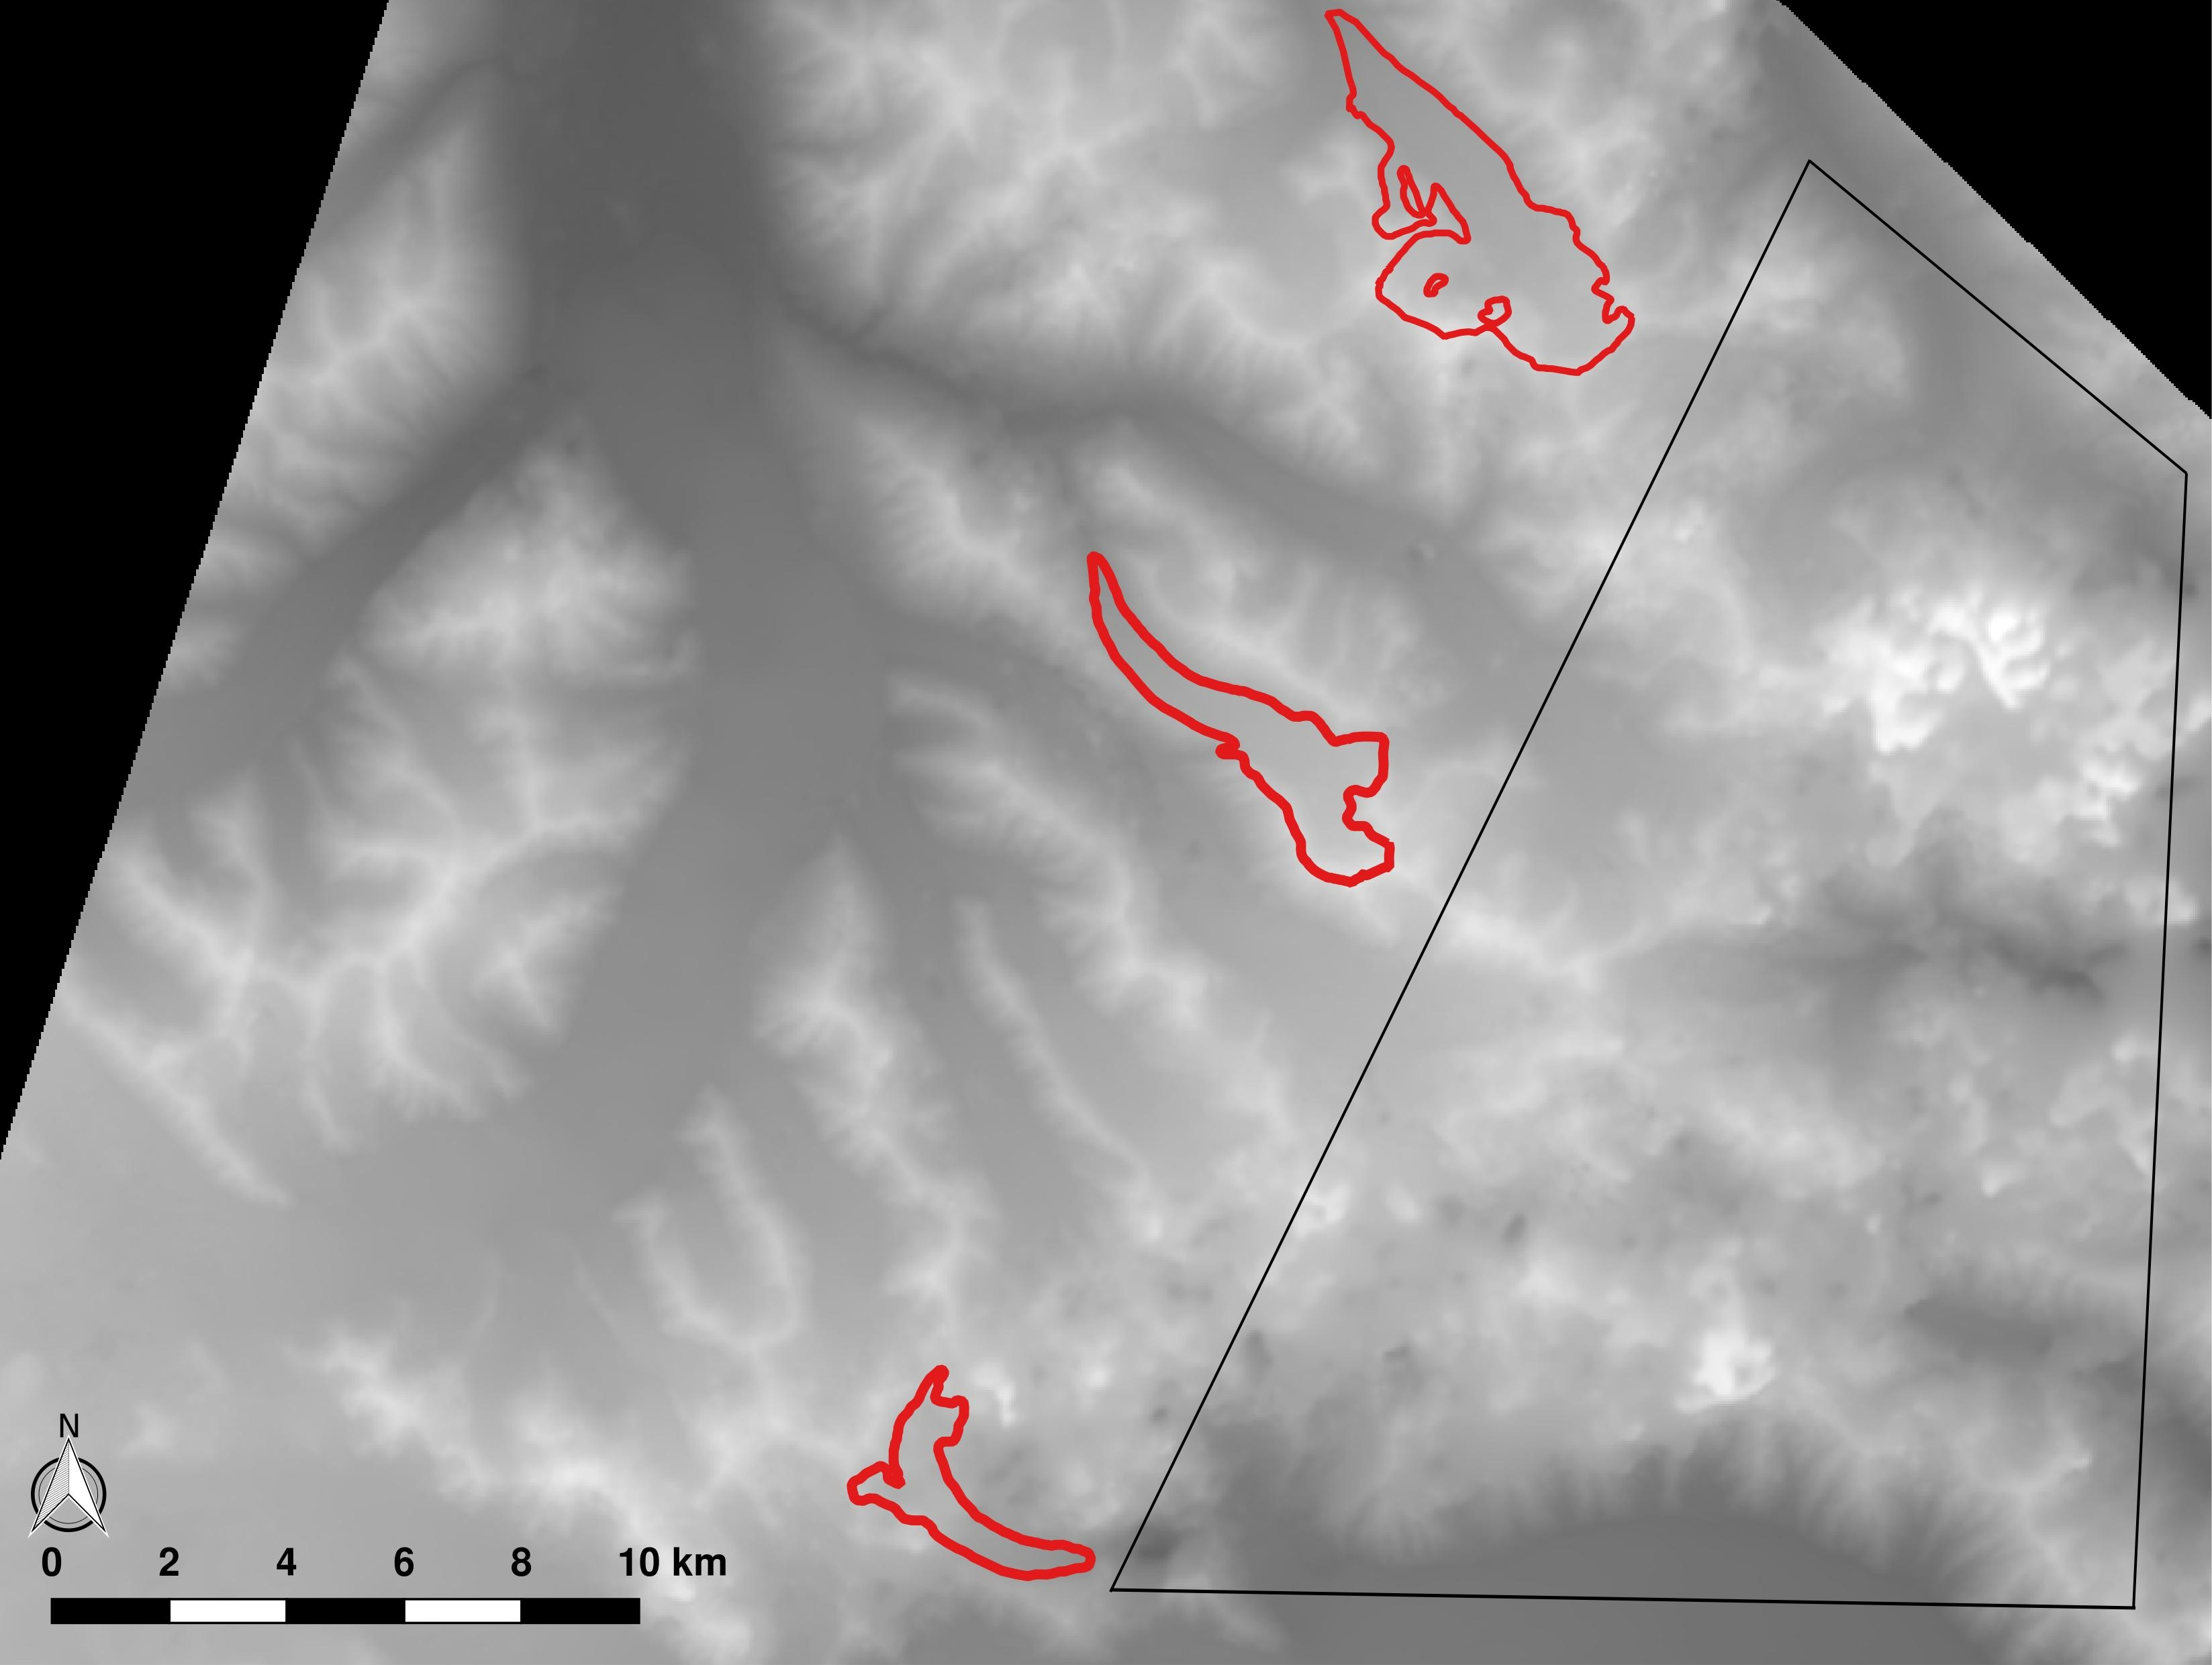
\includegraphics[width=\textwidth]{8029_original2.jpeg}}
        \caption{}
        \label{fig:8029_original}
    \end{subfigure}
    ~
    \begin{subfigure}[b]{0.48\textwidth}
        \fbox{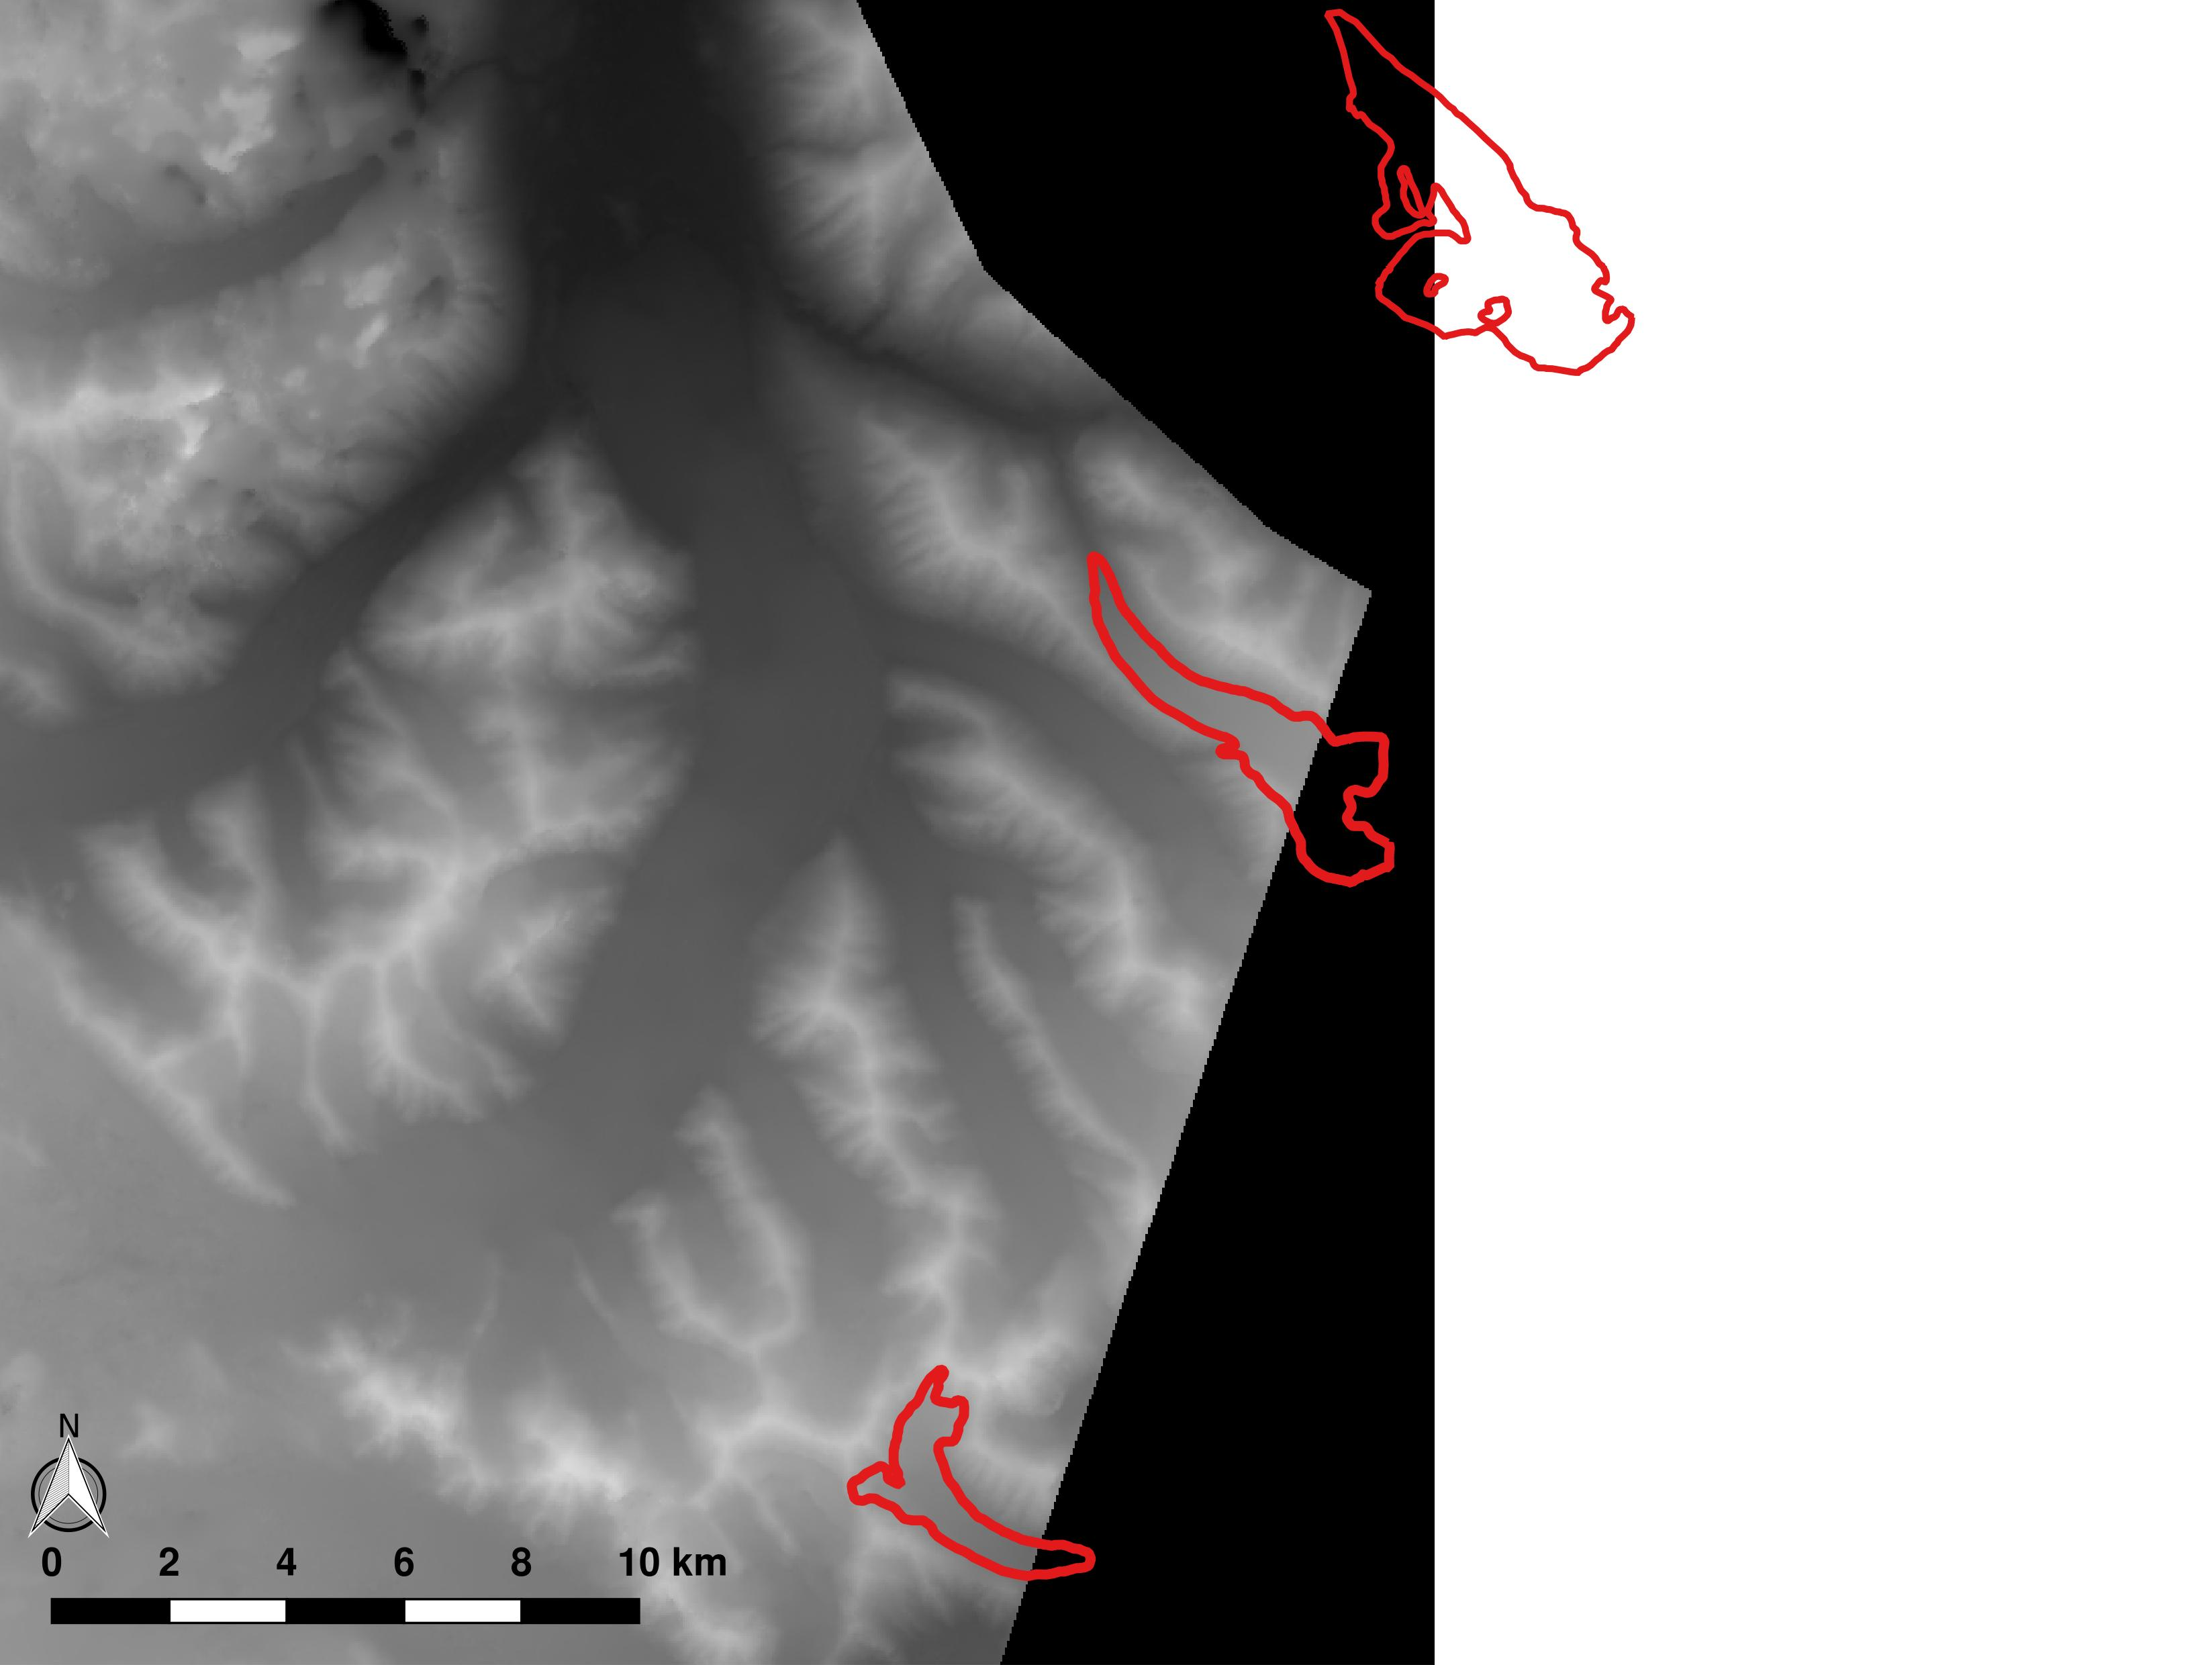
\includegraphics[width=\textwidth]{7044_original.jpeg}}
        \caption{}
        \label{fig:7044_original}
    \end{subfigure}

    \caption{SPOT-5 DEMs available for the Donjek Range. Study glaciers are shown as red outlines. The DEM made from imagery collected on September 3, 2007 (GES 08-029) is shown in (a) and the DEM made from imagery collected on September 13, 2007 (GES 07-044) is shown in (b). Imagery that contains cloud cover result in a distorted DEM, as seen in the boxed area of (a).}
    \label{photo_swe}
\end{figure}

\begin{figure}[H]
  \makebox[\textwidth][c]{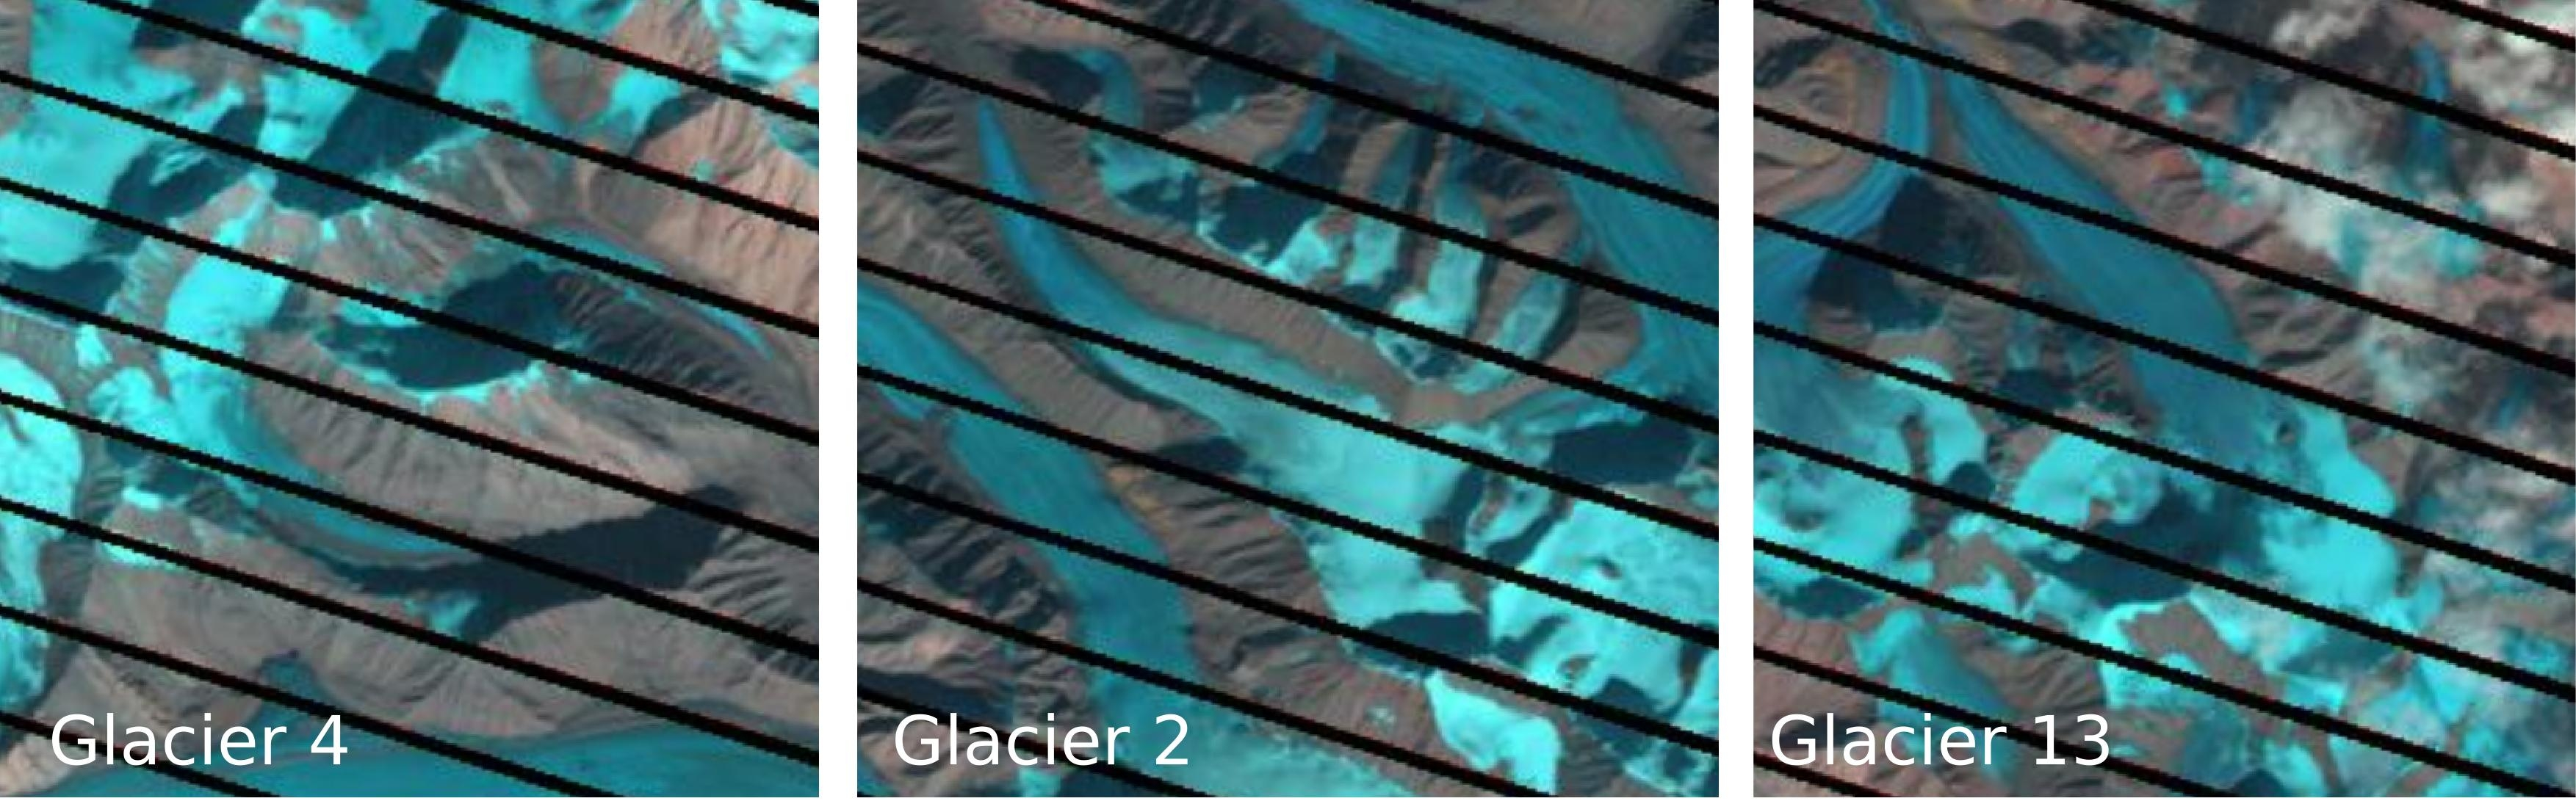
\includegraphics[width=\textwidth]{Landsat_2007.jpeg}}%
	\caption{Landsat 7 ETM images of study glaciers on September 13, 2007. Snow cover is shown as light blue and ice is shown as dark blue.}
	\label{fig:Landsat_2007}
\end{figure}

The GES 08-029 DEM coveres all three study glaciers (see Figure \ref{fig:8029_original}) but a large part of Glacier 4 and some areas of Glacier 2 were masked by clouds and/or showed limited contrast in the original steroimage pairs, resulting in incorrect elevation data (E. Berthier personal communication, 2016). The cloudy areas appear as black regions on the DEM mask (not shown) and as distortion in the DEM, as seen in the boxed area of Figure \ref{fig:8029_original}. The second DEM (GES 07-044)  spans only part of the Donjek Range, covering most of Glacier 4 and $\sim$60\% of Glacier 2 (see Figure \ref{fig:7044_original}). This DEM had no masked areas over Glaciers 2 and 4. The two DEMs were therefore merged to create a cloud free DEM that spanned all three glaciers. 

\begin{figure}[H]
    \centering
    \begin{subfigure}[b]{0.48\textwidth}
        \fbox{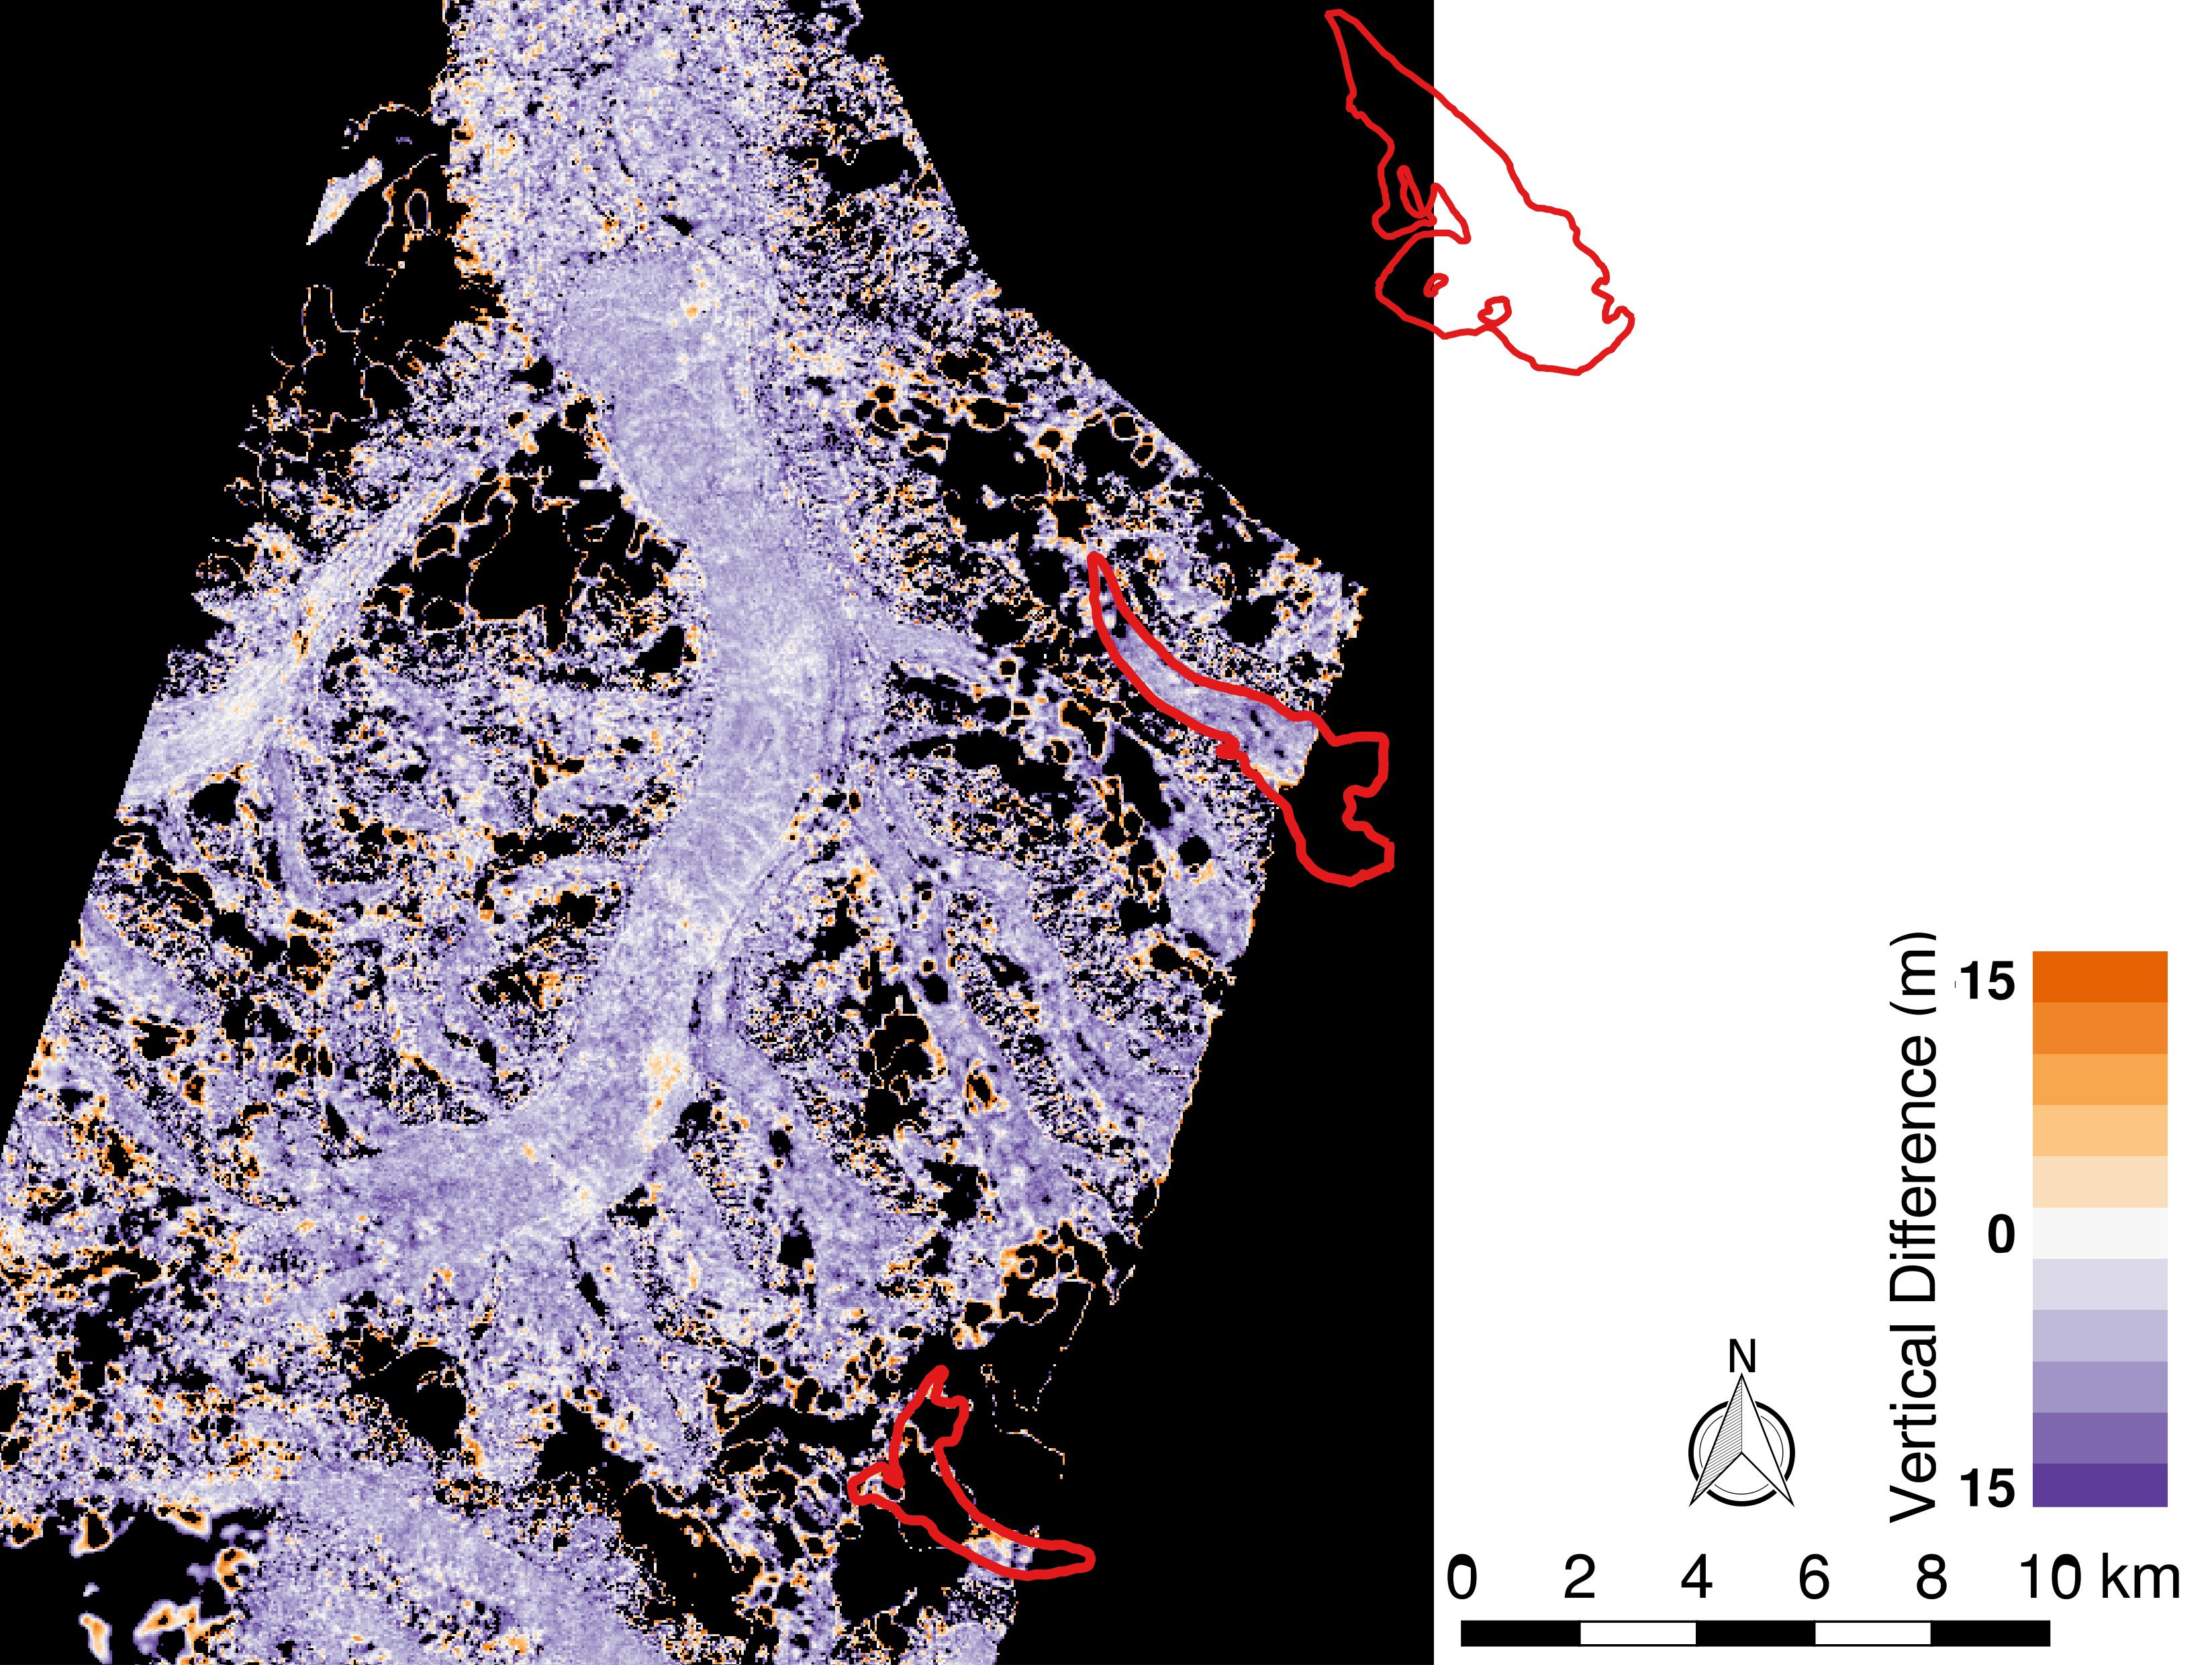
\includegraphics[width=\textwidth]{diff_7044-8029_original.jpeg}}
        \caption{Difference between original DEMs}
        \label{fig:DEMdifferenceOriginal}
    \end{subfigure}
    ~
    \begin{subfigure}[b]{0.48\textwidth}
        \fbox{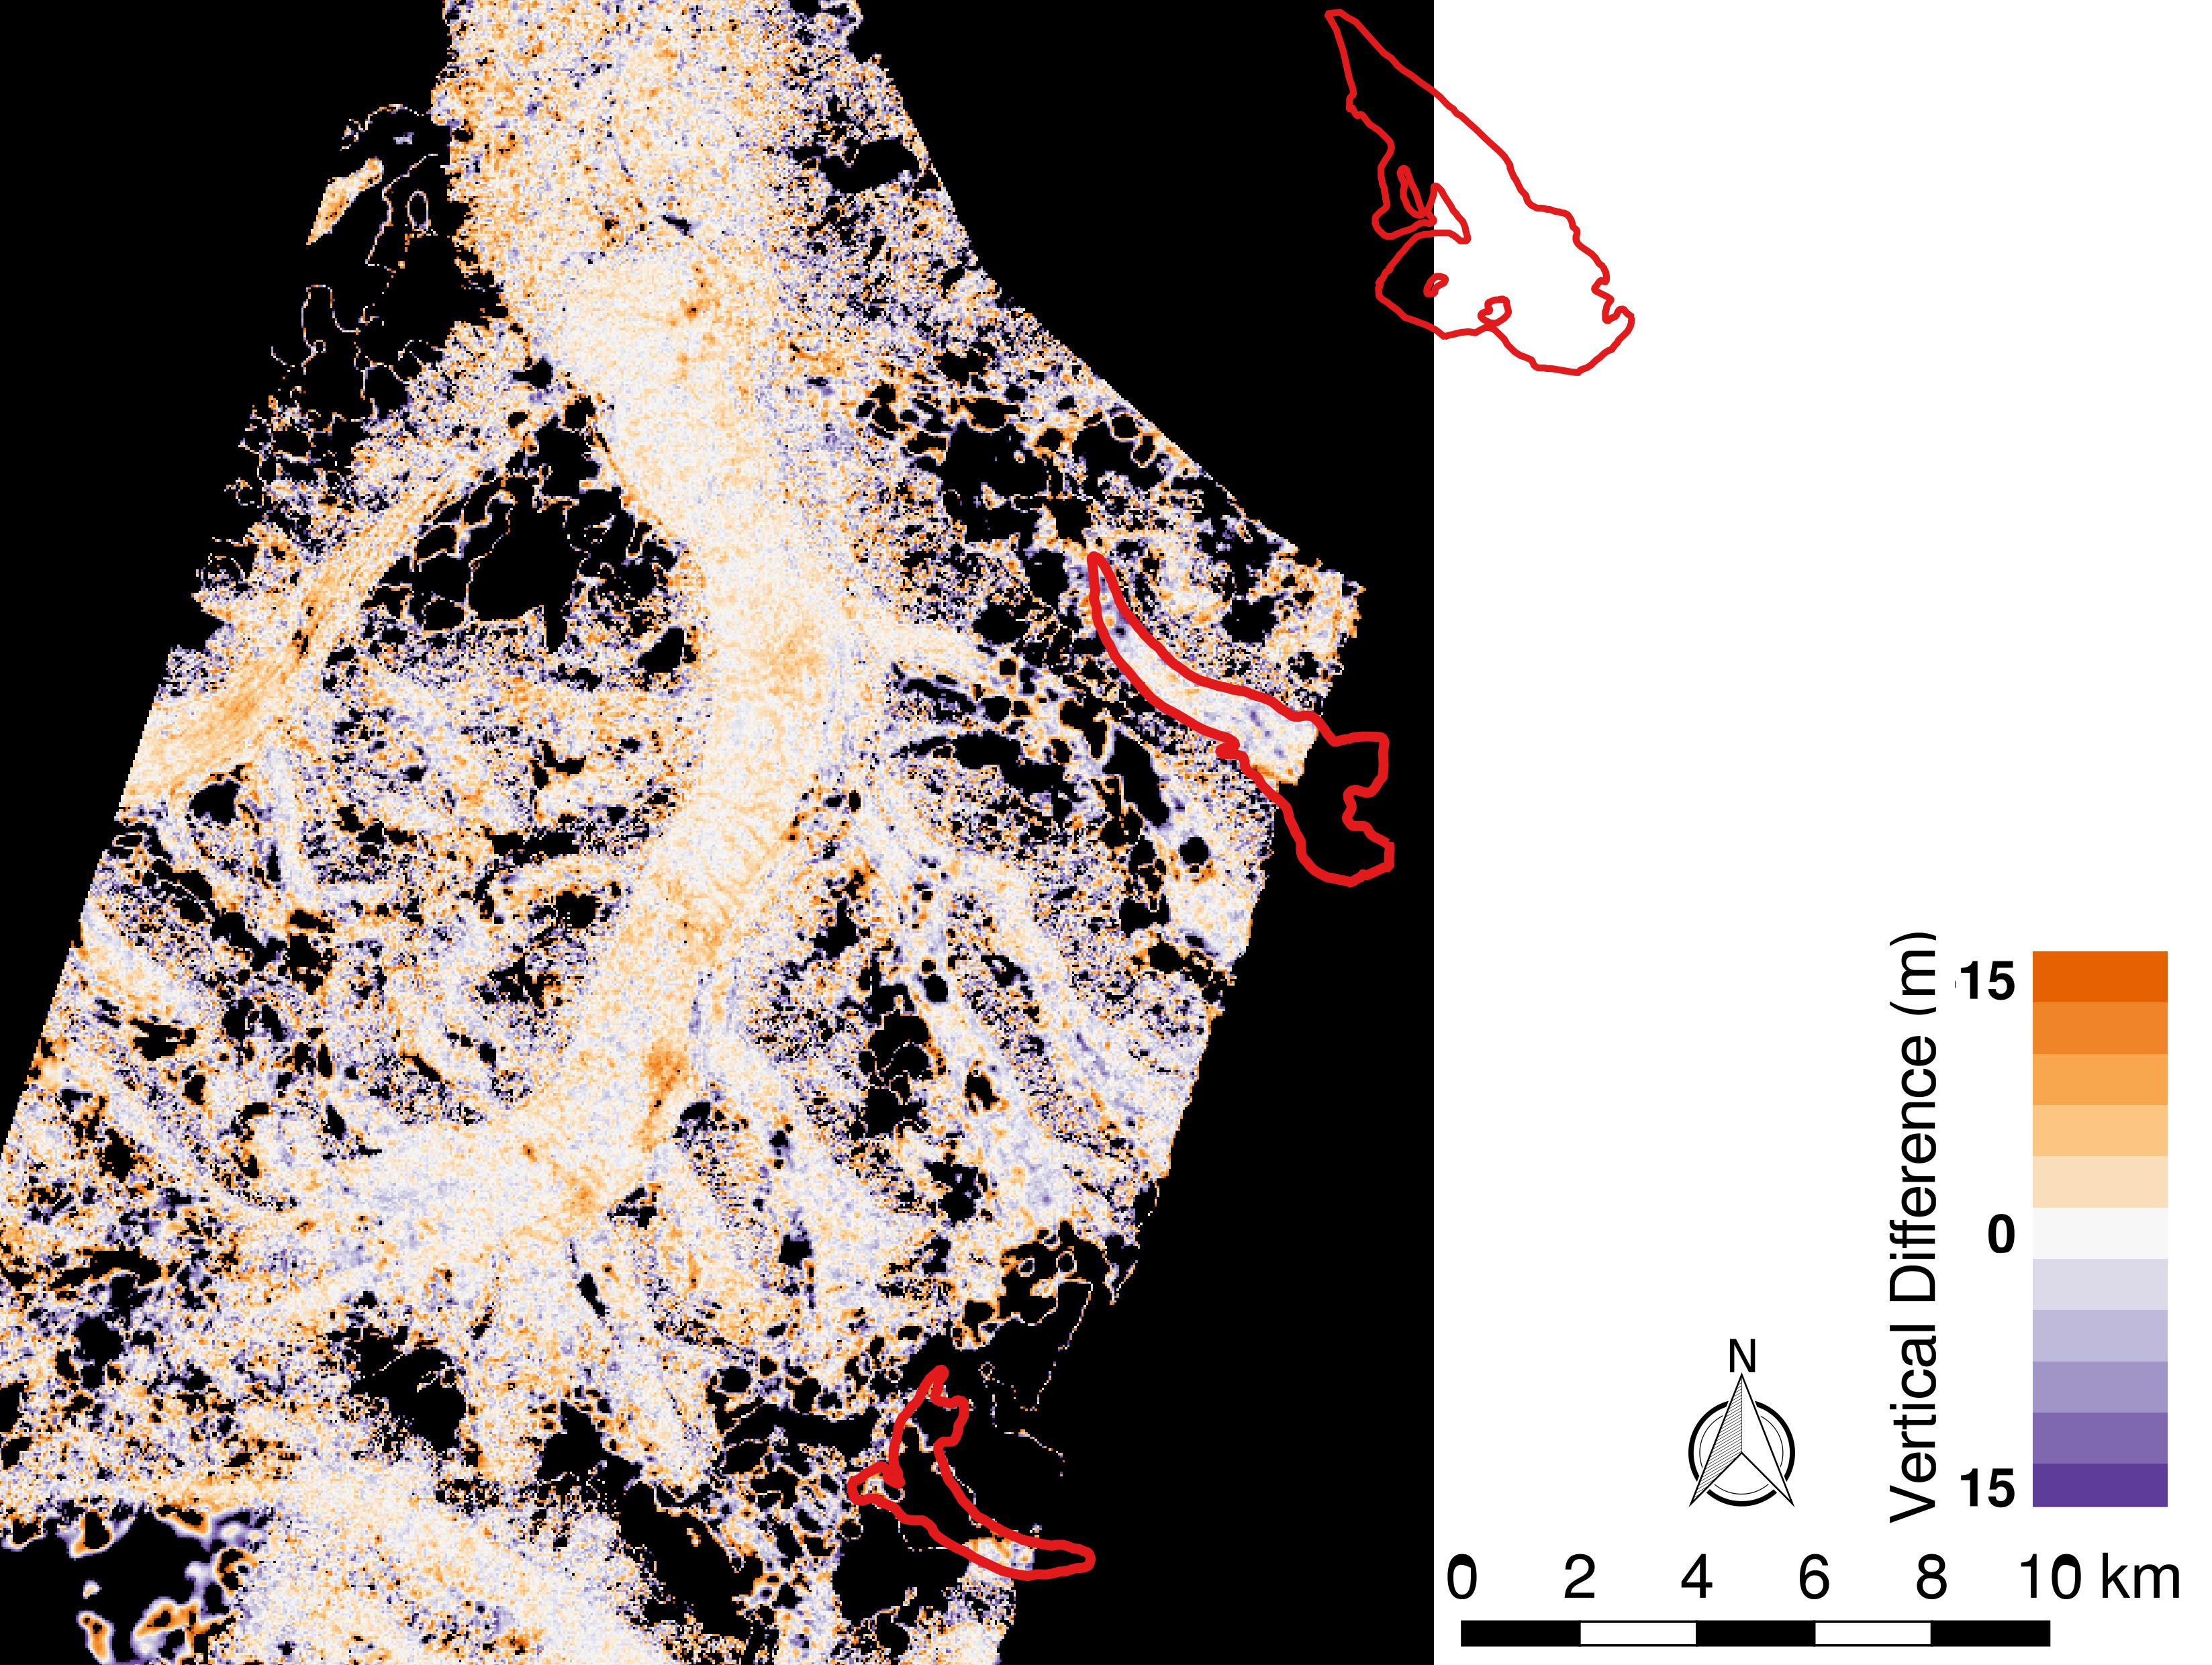
\includegraphics[width=\textwidth]{diff_7044-8029_shift.jpeg}}
        \caption{Difference between corrected DEMs.}
        \label{fig:DEMdifferenceCorrected}
    \end{subfigure}

    \caption{Vertical difference between DEMs in overlapping area. Difference was found by subtracting GES 08-029 from GES 07-044. Positive values indicate that GES 07-044 values are higher than GES 08-029 values. }
    \label{fig:DEMdifference}
\end{figure}

The merging process was complicated by the fact that there was a horizontal and vertical discrepancy between the two DEMs. Although the discrepancy was not consistent throughout the study area, the GES 07-044 DEM was generally higher than the first, as can be seen by the overall purple colour in Figure \ref{fig:DEMdifferenceOriginal}. 


\begin{wrapfigure}{R}{0.6\textwidth}
	\centering
	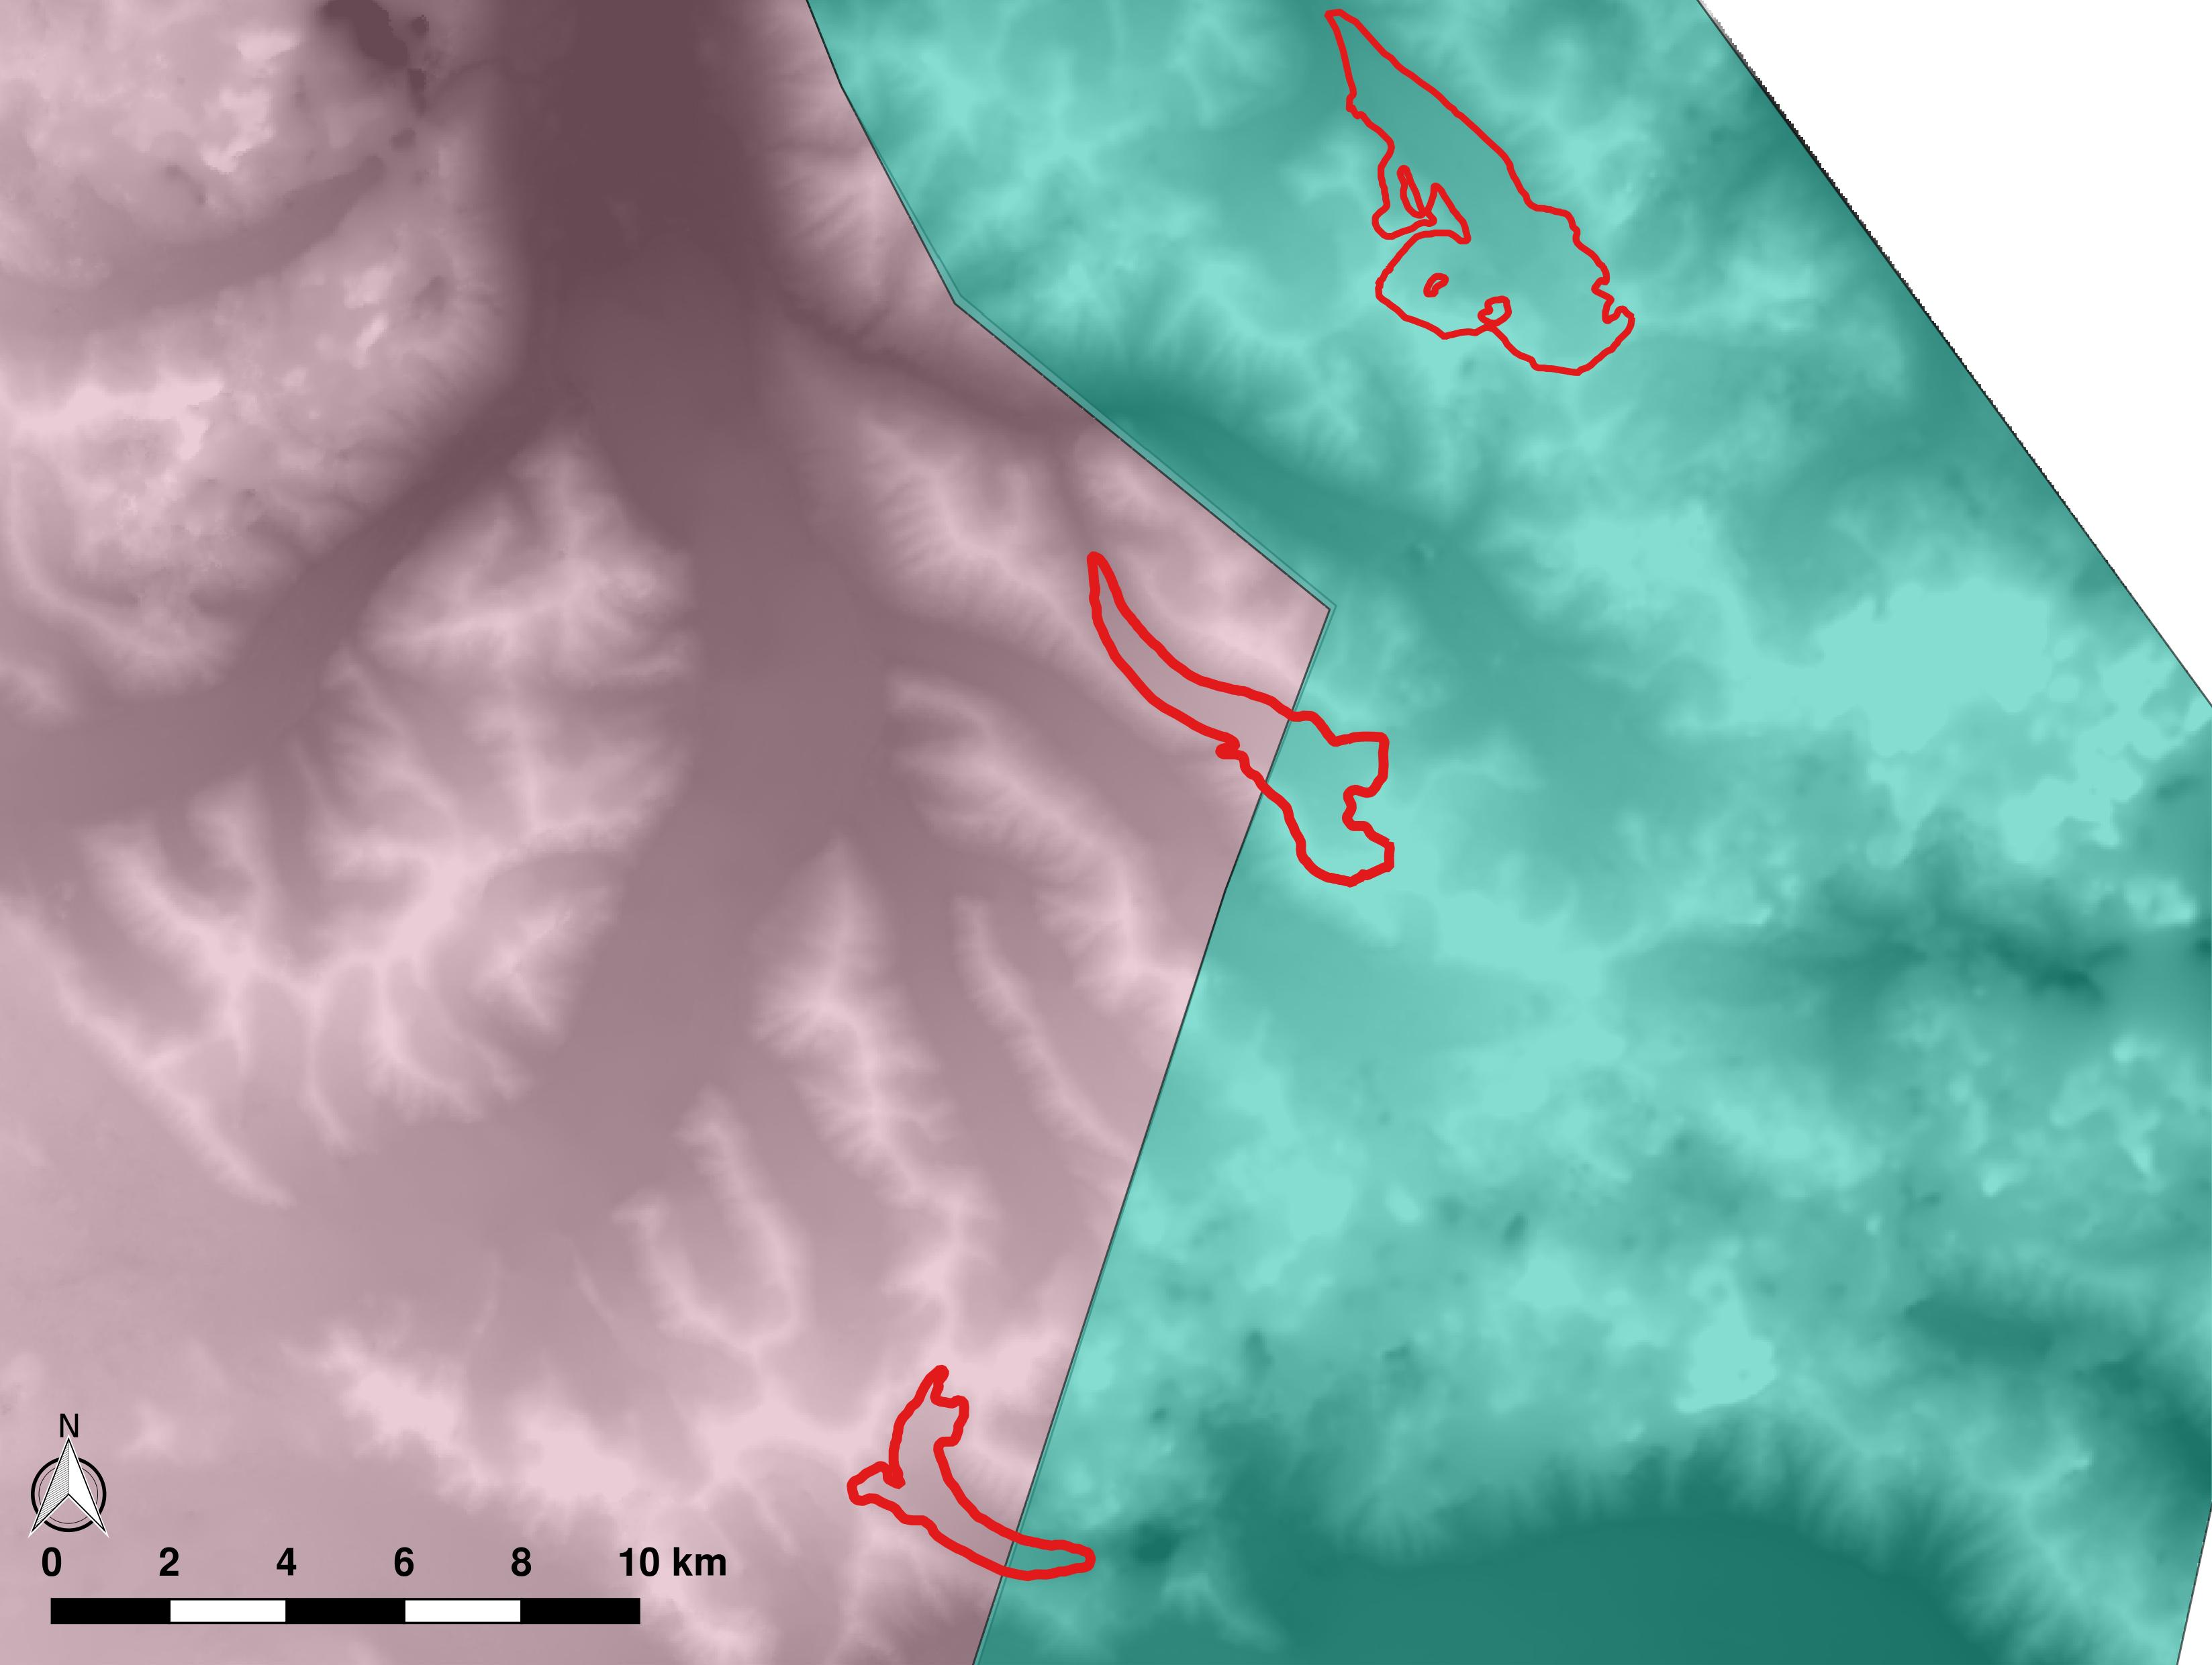
\includegraphics[width = 0.6\textwidth]{mergeLine.jpeg}\\
	\caption{Outlines of the cropped GES 07-044 DEM (pink, left) and cropped GES 08-029 DEM (blue, right) used for merging. There is a slight overlap between the two DEMs that cannot be seen at this scale.}
	\label{fig:mergeLine}
\end{wrapfigure}

The discrepancy was corrected by E. Bertier (2016, personal communication) using an iterative 3D-coregistration algorithm \citep{Berthier2007}. The GES 07-044 DEM was arbitrarily chosen to be used as the reference DEM. Note that the absolute value of the elevation is not necessarily important for the topographic regression, as long as the relative elevations are correct. The reference DEM, GES 07-044, was first shifted vertically by +5.4 m, estimated using ICESat data \citep{Berthier2010}. Then, the mean horizontal and vertical (X, Y, Z) shift between the reference DEM and the GES 08-029 DEM was found by minimizing the standard deviation of the elevation differences between the DEMs. Using this correlation, the GES 08-029 DEM  was shifted $\sim$2 m east, $\sim$4 m north, and $\sim$1.9 m vertically. The GES 08-029 DEM was then reprojected in the same projection as the reference DEM (GES 07-044). The difference map between the two shifted DEMs is shown in Figure \ref{fig:DEMdifferenceCorrected}. Difference values are not uniform but do show both positive and negative values.

Merging of the corrected DEMs was completed in QGIS. First, the rasters were cropped to overlap by a few cells. The crop line was chosen by hand to include as much of the reference DEM as possible (fewer areas of poor data) but was a relatively small distance from the edge of the DEM (see Figure \ref{fig:mergeLine}). The second DEM was cropped to follow the same merge line but overlap with the first DEM by a few cells. This was done to avoid gaps in cell values that arise from cropping across a DEM cell. The merging was completed using the built in QGIS tool `Merge' and in areas where the two DEMs overlapped, the GES 08-029 DEM values were chosen.

The final DEM used for subsequent analysis can be seen in Figure 4. Despite the corrections, there were still discrepancies along the intersection of the DEMs, which can be seen as sharp boundaries in the contour lines. However, these discrepancies are not present on the study glaciers and are located more than 250 m from the edge of the glacier so this DEM was used as the final version for the Donjek Range.

\begin{figure}
\begin{adjustbox}{addcode={\begin{minipage}{\width}}{\caption{%
      Merged DEM of the Donjek range from two corrected SPOT-5 DEMs, plotted with 10 m contour lines. Study glaciers are shown in red. Discrepancies between the DEMs along the merge line can be seen as anomalous linear features in the contour map (yellow boxes). Distorted contours in the eastern regions (white box) are a result of errors in the DEM. 
      }\end{minipage}},rotate=90,center}
     	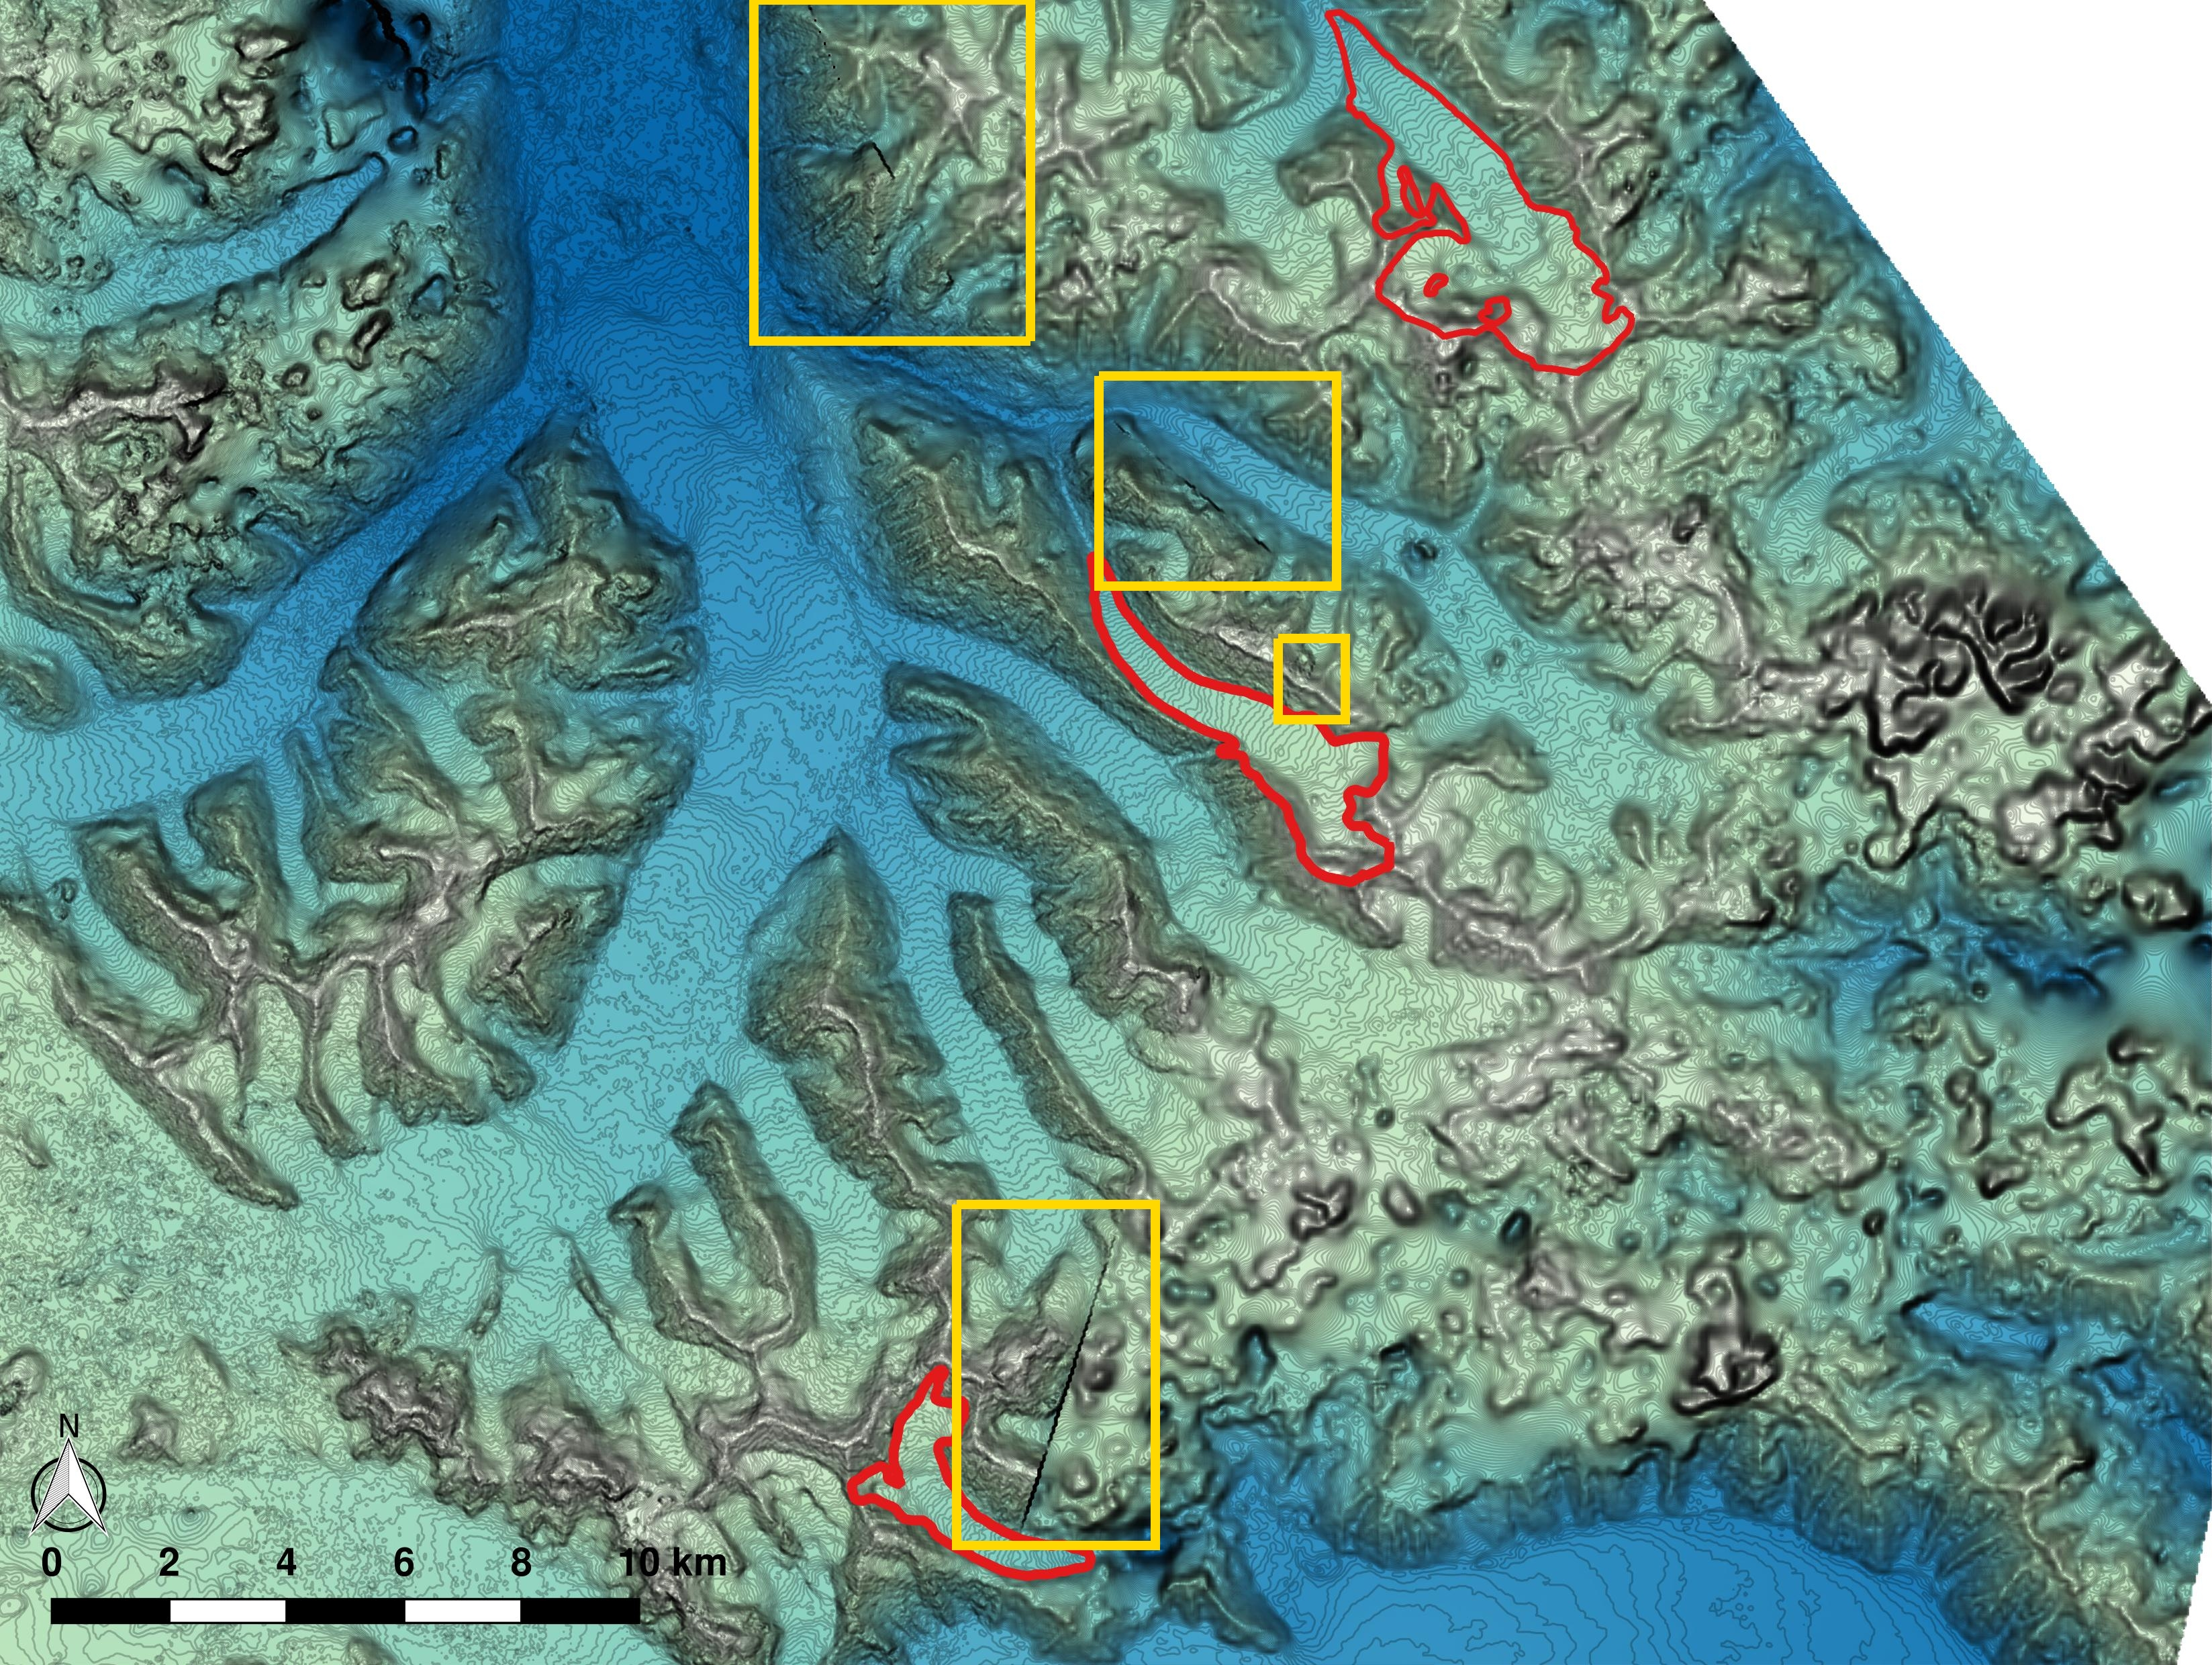
\includegraphics[height = 0.9\textwidth]{mergedDEM2.jpeg}%
 \end{adjustbox}  
  \label{fig:finalDEM}
\end{figure}

\subsection{Calculating topographic parameters}
\label{sec:topoCalc}

Topographic parameters are used to describe characteristics of the local topography that may affect snow distribution and can act as proxies for physical processes that determine snow deposition and redistribution. Topographic parameters used in snow accumulation studies on glaciers include elevation ($z$), distance from centreline ($d_C$), slope ($m$), tangential ($\kappa_T$) and profile ($\kappa_P$) curvature, ``northness'' ($N$), aspect ($\alpha$), and $Sx$, which is a proxy for wind redistribution \citep{Basist1994, Revuelto2014, McGrath2015}.	
 
A number of programs were used calculate topographic parameters from the DEM. Distance from centreline and ``northness'' were calculated in Matlab. $Sx$ was determined using a executable obtained from Adam Winstral that follows the procedure outlined in \cite{Winstral2002}. The remaining parameters were calculated using the \texttt{r.slope.aspect} module in GRASS GIS software run through QGIS as described in \cite{Mitavsova1993} and \cite{Hofierka2009}. 

The GRASS module implements a local polynomial approximation method of the form 
\begin{equation}
z(x,y) = a\cdot x^2 +b\cdot y^2 +c \cdot x\cdot y +d \cdot x + e\cdot y +f.
\end{equation}•
This polynomial is fitted to 9 grid points (3$\times$3 array) and the coefficients are determined by weighted least squares. 
First order partial derivatives are derived using Horn's formula \citep{Horn1981, Neteler2013}. The gradient can be expressed as
\begin{equation}
\nabla \bar{ \bm{z}} = \left( \frac{\partial z}{\partial x}, \frac{\partial z}{\partial y} \right) = \left( 2 \cdot a  \cdot x + c  \cdot y +d, 2 \cdot b  \cdot y + c  \cdot x + e \right) .
\end{equation}•
Since we are interested in the value of the centre cell ($x=y=0$), the gradient is simply 
\begin{equation}
\nabla \bar{ \bm{z}} = (f_x,f_y) = (d,e),
\end{equation}•
where $d$ and $e$ are given by
\begin{equation}
f_x = \frac{(z_7-z_9)+(2z_4-2z_6)+(z_1-z_3)}{8 \cdot \Delta x},\\
\end{equation}•
\begin{equation}
f_y = \frac{(z_7-z_1)+(2z_8-2z_2)+(z_9-z_3)}{8 \cdot \Delta y}.
\end{equation}•
Here, $z_k$ refers to one of the grid cells surrounding the cell of interest, which is located at row $i$ and column $j$ of the DEM. So $z_3 = z_{i+1,j+1}$, $z_7 = z_{i-1,j-1}$, and so on. $\Delta x$ and $\Delta y$ are the grid spacing (resolution) of the DEM. The second order partial derivatives can be written as \citep{Hofierka2009, Neteler2013}
\begin{align}
f_{xx} &= \frac{z_1-2z_2+z_3+4z_4-8z_5+4z_6+z_7-2z_8+z_9}{6 \cdot (\Delta x)^2},\\
f_{yy} &= \frac{z_1-4z_2+z_3-2z_4-8z_5-2z_6+z_7+4z_8+z_9}{6 \cdot (\Delta y)^2},\\
f_{xy} &= \frac{(z_7-z_9)-(z_1-z_3)}{4 \cdot \Delta x \Delta y}.
\end{align}
The second derivatives are most commonly used to calculate the curvature of a surface. The curvature at a given point on a curve is determined by finding the inverse of the radius of a circle that best fits the curve \citep{Olaya2009}. Convex surfaces have positive curvature and concave surfaces have negative curvature. 

Details about the calculation of topographic parameters are described below.
\begin{enumerate}
\item[]\textbf{Elevation} values were taken from the (corrected) SPOT-5 DEMs directly.

\item[] \textbf{Distance from centreline} was calculated as the minimum distance between the Easting and Northing of the northwest corner of each cell and a centreline that was drawn by hand in QGIS. This was completed in Matlab using the script `CentrelineDistance.m'. 

\item[]  \textbf{Slope} is taken to be the steepest slope angle and is the magnitude of gradient \citep{Mitavsova1993}. Using the gradient, it can be expressed as  \citep{Olaya2009}
	\begin{equation}
	m = \textrm{arctan}(|\nabla \bar{ \vector{z}}|) = \textrm{arctan} \left( \sqrt{(f_x)^2 +( f_y)^2} \right)
	\end{equation}•
\item[] \textbf{Tangential Curvature} (horizontal curvature) represents the curvature in the direction of the contour tangent. The equation for tangential curvature can be written as \citep{Olaya2009}
	\begin{equation}
	\kappa_T = - \frac{e^2 \cdot r -2 \cdot d\cdot e \cdot s +d^2 \cdot t}{(d^2+e^2) \cdot \sqrt{1+d^2+e^2}}
	\end{equation}•
where $d$ and $e$ are as above and
	\begin{align}
	r &= \frac{\partial^2 z}{\partial x^2} = \frac{z_1+z_3+z_4+z_6+z_7+z_9-2 \cdot (z_2+z_5+z_8)}{3 \cdot \Delta s^2}\\
	s &= \frac{\partial^2 z}{\partial x \partial y} = \frac{z_3 + z_7- z_1 - z_9}{4 \cdot \Delta s^2}\\
	t &= \frac{\partial^2 z}{\partial y^2} = \frac{z_1+z_2+z_3+z_7+z_8+z_9-2 \cdot (z_4+z_5+z_6)}{3 \cdot \Delta s^2}
	\end{align}•	

\item[] \textbf{Profile Curvature} (vertical curvature) represents the curvature in the direction of the the steepest slope (gradient). The equation for profile curvature can be written as \citep{Olaya2009}
	\begin{equation}
	\kappa_P = - \frac{d^2 \cdot r +2 \cdot d\cdot e \cdot r \cdot s +e^2 \cdot t}{(d^2+e^2) \cdot \sqrt{(1+d^2+e^2)^3}}
	\end{equation}•

\item[] \textbf{``Northness''} is a solar radiation parameter that has been shown to become increasingly important during the spring \citep{Revuelto2014}. It is also likely that this parameter may be related to sun induced snow metamorphosis and/or sun crusts, both of which affect SWE and snow redistribution \citep{McGrath2015}. ``Northness'' is defined as the product of the cosine of aspect and sine of slope \citep{Molotch2005}. A value of -1 represents a steep, south facing slope, a value of +1 represents a steep, north facing slope, and a flat surfaces yield 0. 

\item[] \textbf{Aspect} represents the orientation of the steepest slope, with 0${^\circ}$ defined as north and no value given to cells that have no gradient. Using the gradient, it can expressed as \citep{Olaya2009}
	\begin{equation}
	\alpha = 180 - \textrm{arctan}\left(\frac{ f_y}{ f_x}\right)+90 \cdot \frac{ f_x}{| f_x|}
	\end{equation}•

\item[] \textbf{\textit{Sx}} represents wind exposure/shelter and is based on selecting a cell within a certain angle and distance from the cell of interest that has the greatest upward slope relative to the cell of interest \citep{Winstral2002}. This can be referred to as the maximum upwind slope. Negative $Sx$ values represent exposure relative to the shelter-defining pixel, which means that the cell of interest was higher than the cell with greatest upward slope. Conversely, positive values represent sheltered cells. To determine $Sx$ values, we use the equation
\begin{equation}
Sx_{A, dmax}(x_i, y_i) = \textrm{max} \left[ \textrm{tan}^{-1} \left( \frac{z(x_v,y_v)-z(x_i,y_i)}{[(x_v-x_i)^2+(y_v-y_i)^2]^{1/2}} \right) \right] ,
\end{equation}
where A is the azimuth of the search direction, $(x_i, y_i)$ are the coordinates of the cell of interest, and $(x_v, y_v)$ are the set of all cell coordinates located along the search vector defined by	$(x_i, y_i)$, the azimuth ($A$), and maximum search distance ($d$max). Code for this calculation was provided by Adam Winstral (2016, personal communication). As done by \cite{McGrath2015}, we computed $Sx$ at 5$^{\circ}$ azimuth increments for $d$max distances of 100, 200, and 300 m. These values were then correlated with observed values of SWE and the azimuth and $d$max values with the highest correlation were used for subsequent analysis (see Table \ref{tab:Sxparams}). The code for calculating $Sx$ requires a UTM raster formatted to ASCII in ArcGIS. 
\end{enumerate}

\begin{table}[H]
\centering
\caption{Values of azimuth ($A$) and maximum search distance ($d$max), that correspond to the $Sx$ that had the highest absolute correlation to observed SWE.}
\label{tab:Sxparams}
\begin{tabular}{lccc}
 & \begin{tabular}[c]{@{}c@{}}$A$\\ ($^{\circ}$ from North)\end{tabular} & \begin{tabular}[c]{@{}c@{}}$d$max \\ (m)\end{tabular} & \begin{tabular}[c]{@{}c@{}}Correlation\\ Coefficient\end{tabular} \\ \hline
Glacier 4 & 85 & 300 & $-$0.26 \\
Glacier 2 & 330 & 300 & 0.56 \\
Glacier 13 & 280 & 200 & 0.28
\end{tabular}
\end{table} 


\subsection{Topographic parameters from QGIS to Matlab}

The value of each topographic parameter at the sampling locations was determined in QGIS. The sampling locations were imported to QGIS and the Point Sampling Tool was used to determine the value of the topographic parameter raster cell at each measurement location. The set of parameters that corresponds to e`ch location was then exported to a .csv file and imported into Matlab with the script 'Import\_Topo.m'.  Note that selection of $Sx$ values was completed first (see above) and only the $Sx$ values with highest correlation to SWE was exported. After importing to Matlab, the sets of parameter values ($x_p$) were standardized ($x_s$) by $x_s = \frac{x_p-\mu}{\sigma}$. The resulting structure is called \texttt{topo\_sampled} and is used in the MLR to be able to compare the explanatory power of each parameter (Section \ref{sec:MLR}). A non-standardized copy of the topographic parameters at the sampling locations was also kept for plotting purposes and is called is called \texttt{topo\_sampled\_ns}. Both structures are organized as a vector of values corresponding to the vectors in the \texttt{SWE} variable. 

The topographic parameter rasters were also exported from QGIS as a .csv file and then imported into Matlab with the script `Import\_Topo.m'. The values are stored in the structure \texttt{topo\_full}, where each cell corresponds to one DEM cell. Cells outside of the glacier outline have no value (\texttt{NaN}). The raster values were standardized using the mean and standard deviation of the sampled topographic parameters so that this set of full topographic parameters could be used for modelling SWE using the regression. A copy of the non-standardized values was stored as \texttt{topo\_full\_ns}.

\subsection{Parameter correlations}

The correlation between topographic parameters at sampling locations on each glacier is shown in Table \ref{tab:pearson_correlation}. Correlation values are generally low, with the exception of the correlation between northness and aspect on Glacier 2 and northness and $Sx$ on Glacier 13, which were both larger than 0.7. Since there is little correlation between parameters and the correlations vary between glaciers, the use of a linear regression with these topographic parameters as predictor variables is warranted. 

\begin{table}[H]
\centering
\caption{Pearson correlation coefficients between topographic parameters at sampled locations. \params}
\label{tab:pearson_correlation}
\begin{tabular}{cc|cccccccc}
 &  & $d_C$ & $z$ & $\alpha$ & $m$ & $N$ & $\kappa_P$ & $\kappa_T$ & $Sx$ \\ \hline
 
 & $d_C$ & 1 & 0.20 &  $-$0.28 & 0.36 & 0.11 &  $-$0.19 &  $-$0.13 & 0.37 \\
 
 & $z$ & & 1 & 0.27 &  $-$0.11 &  $-$0.35 & 0.13 & 0.04 & 0.36 \\
 
 & $\alpha$ & & & 1 &  $-$0.29 &  $-$0.24 & 0.19 & 0.07 & 0.22 \\
 
 & $m$ & & & & 1 & 0.55 &  $-$0.36 &  $-$0.09 & 0.03 \\
 
 & $N$ & & & & & 1 &  $-$0.16 &  $-$0.03 &  $-$0.47 \\
 
 & $\kappa_P$ & & & & & & 1 & 0.41 &  $-$0.18 \\
 
 & $\kappa_T$ & & & & & & & 1 &  $-$0.28 \\
 
\multirow{ -8}{*}{Glacier 4} & $Sx$ & & & & & & & & 1 \\ \hline
 & $d_C$ & 1 & 0.05 &  $-$0.22 & 0.11 & 0.24 & 0.07 & 0.20 &  $-$0.01 \\
 & $z$ & & 1 & 0.56 &  $-$0.49 &  $-$0.32 & 0.08 & 0.03 & 0.58 \\
 & $\alpha$ & & & 1 &  $-$0.39 &  $-$0.72 & 0.19 & 0.04 & 0.49 \\
 & $m$ & & & & 1 & 0.04 &  $-$0.03 &  $-$0.02 &  $-$0.37 \\
 & $N$ & & & & & 1 &  $-$0.19 &  $-$0.03 &  $-$0.11 \\
 & $\kappa_P$ & & & & & & 1 & 0.44 &  $-$0.23 \\
 & $\kappa_T$ & & & & & & & 1 &  $-$0.27 \\
\multirow{ -8}{*}{Glacier 2} & $Sx$ & & & & & & & & 1 \\ \hline
 
 & $d_C$ & 1 & 0.13 &  $-$0.09 & 0.06 & 0.01 & 0.10 & 0.03 & 0.05 \\
 
 & $z$ & & 1 &  $-$0.11 &  $-$0.01 & 0.30 & 0.06 &  $<$0.01 & 0.31 \\
 
 & $\alpha$ & & & 1 & 0.01 &  $-$0.59 &  $-$0.01 &  $-$0.13 &  $-$0.47 \\
 
 & $m$ & & & & 1 &  $-$0.26 & $<$0.01 &  $-$0.10 &  $<$0.01 \\
 
 & $N$ & & & & & 1 &  $-$0.07 &  $-$0.11 & 0.76 \\
 
 & $\kappa_P$ & & & & & & 1 & 0.36 &  $-$0.30 \\
 
 & $\kappa_T$ & & & & & & & 1 &  $-$0.47 \\
 
\multirow{-8}{*}{Glacier 13} & $Sx$ & & & & & & & & 1
\end{tabular}
\end{table}


\subsection{Maps of topographic parameters and distribution of parameters sampled}


Elevation maps (Figure \ref{map:elev}) show that both Glacier 2 and 13 have small areas with high elevation, which correspond to steep headwalls. Mean elevation is the same for all glaciers for the full and sampled distribution within one standard deviation (Table \ref{tab:sampled&fullParams_stats}). However, maximum elevation values are lower for Glacier 4 than the other two glaciers (Figure \ref{sampledRange:elev}) and the sampled elevation means are approximately 200 m less than that of the full distribution. Standard deviations are smaller for sampled ranges for all glaciers. The skewness of sampled and full distributions is similar for Glacier 2 but differs considerably for Glacier 4 and 13. Elevation full distributions are similar for the study glaciers, with kurtosis for all distributions, except sampled elevation on Glacier 13, being less than 3 (value for normal distribution). Kurtosis of sampled distributions show that Glacier 13 had a broader distribution and Glacier 2 has a narrower distribution. 

The distribution of sampled distance from centreline (Figure \ref{sampledRange:centreD}) is different from that of the full distribution. Generally, large distance were not sampled. Larger values of skewness and kurtosis in the full distribution indicate that these distributions are broader and span a larger range of values (Table \ref{tab:sampled&fullParams_stats}). This is also seen in the mean and standard deviation values, which are also larger for the full distribution. Large values of distance from centreline are located at the edges of the glacier in the accumulation area (Figure \ref{map:centreD}), which constitute steep, inaccessible terrain. Within the ablation area, the hourglass sampling pattern allowed for locations across the whole width of the glacier to be measured. Note that Glacier 13 has two centrelines in the accumulation area because of the confluence of two major arms of the glacier.

Slope of the three study glaciers (Figure \ref{map:slope}) is generally less than 20$^{\circ}$, with only the margins of the accumulation area and a few steps on Glacier 13 having steep slopes. The full and sampled distributions of slope are similar between glaciers (Table \ref{tab:sampled&fullParams_stats}), with mean values between 12$^{\circ}$ and 15$^{\circ}$ for the full distribution and 5$^{\circ}$ to 8$^{\circ}$ for the sampled distribution. The sampled distributions are all different than the full range, as indicated by the lower means, standard deviations, and skewness, as well as larger kurtosis. This shows that the sampled distributions are generally narrower than full distributions and severely under samples steep slopes (Figure \ref{sampledRange:slope}).


$Sx$ maps over the study glaciers are shown in Figure \ref{map:Sx} and the wind direction and maximum search distance with the highest correlation to SWE for each glacier are shown in Table \ref{tab:Sxparams}. For Glacier 4, an approximately east wind and 300 m search distance were most strongly correlated. The correlation was negative, which means that negative values of $Sx$ (exposure) correspond to areas with larger SWE (more snow). This is counter intuitive and perhaps indicates that $Sx$ is not an appropriate topographic parameter to correlate with SWE on Glacier 4. Despite this, $Sx$ was retained in future analysis for consistency between glaciers. For Glacier 2, a north wind with a 300 m search distance was most strongly correlated and for Glacier 13, a west wind with a 200 m search distance produced the strongest correlation. Both of these correlations were positive, so a more positive $Sx$ value (sheltered) corresponds to higher values of SWE (more snow). The correlation values for Glacier 4 and 2 are low ($<$0.3) which indicates that $Sx$ will likely be insignificant in estimating snow accumulation. The correlation between $Sx$ and SWE on Glacier 2 is higher at 0.56. 

The full distribution of $Sx$ (Figure \ref{sampledRange:Sx}) is different for each glacier and differs greatly between sampled and full distributions. Glacier 2 has a mean less than zero, indicating that a large portion of the glacier has exposed topography (Table \ref{tab:sampled&fullParams_stats}). Glacier 4 and 13 have positive mean values of $Sx$, indicating more sheltered topography. Extreme values of $Sx$ are generally located along the edges of the accumulation areas (Figure \ref{map:Sx}). The sampled distribution mean for Glacier 2 is close to that of its full distribution, while the sampled distribution means of Glacier 4 and 13 are different (negative) than that of the full distribution means (positive). The sampled distribution are more sharply peaked, as indicated by the smaller standard deviation values and larger kurtosis when compared to the full distributions. The skewness also differs for Glaciers 4 and 2, with the sampled distributions skewed more to the right than full distributions. Overall, the sampled distribution of $Sx$ is a poor representation of the full distribution. 


---------

Maps of the topographic parameters for each glacier are shown below. Additionally, the distribution of topographic parameter values and the sampled distribution for each parameter is also shown. The full range of parameters has highest frequencies for Glacier 13 and lowest for Glacier 4 because Glacier 13 is larger than Glacier 4. Frequency of sampled parameters are comparable between glaciers because the sampling schemes were similar.

 




Tangential curvature is shown in Figure \ref{map:tangentC} and profile curvature is shown in Figure \ref{map:profileC}. The curvature values are generally moderate and centred about 0. The distribution of sampled curvature closely matches the full distribution although high curvature areas were not sampled (see Figure \ref{sampledRange:tangentC} and \ref{sampledRange:profileC}).


Aspect of the glacier surface is shown in Figure \ref{map:aspect}. Glacier 2 and 13 have similar aspect distributions, with a mean aspect of $\sim100^{\circ}$. Glacier 4 has a mean aspect of $\sim300^{\circ}$, which is roughly $180^{\circ}$ to that of Glacier 2 and 13. The sampled distribution, as shown in Figure \ref{sampledRange:aspect}, for Glacier 4 follows that of the full distribution relatively well. However, the sampled distribution of Glacier 2 and 13 does not match that of the full distribution and there are many aspects that were not sampled.  


QGIS Aspect: 90 degrees is North, 180 is West, 270 is South 360 is East
Olaya2009 Aspect : 0=N and read clockwise

``Northness'' for all study glaciers is shown in Figure \ref{map:northness}. The majority of cells have values close to zero, which is likely due to their low slope values. Even for Glacier 4, which is largely south facing and should thus have lower values of ``northness'', has a distribution with a mean close to zero. The low slope values mean that the values of ``northness'' were determined largely by the aspect, which can be seen by the resemblance between the ``northness'' map and the aspect map. 



Overall, the sampled topographic parameters are representative of the full distribution of parameters. Extreme values are grossly under sampled so that the full range of parameter values was not sampled. This was largely do to dangerous travel conditions and an inability to quickly and accurately measure snow depth in the accumulation area. As a result, extrapolation of regression models will likely result in large errors. This is especially relevant in the accumulation area, which has extreme values for all parameters. Errors in the accumulation area are especially important to acknowledge because this area has the most accumulation and is likely to heavily influence final winter mass balance values. It is also important to note that for a number of parameters (especially elevation) the sampling distribution is off-set from that of the full distribution. Generally, the sampled values do not fully capture the variance in topographic parameters but a regression is still valuable to conduct since topographic regressions are common when estimating winter mass balance. Acknowledging that this methodology is limited and prone to extrapolation errors is paramount to capturing uncertainty in accumulation studies. 

\begin{landscape}
\begin{table}[]
\small
\centering
\caption{Descriptive statics of topographic parameter full and sampled distribution. Mean and standard deviation are in units of meters for distance from centreline ($d_C$) and elevation ($z$), in units of m$^{-1}$ for profile ($\kappa_P$) and tangential ($\kappa_T$) curvature, and are unitless for cosine of aspect ($\alpha$), ``northness'' ($N$), slope ($m$), and $Sx$. Skewness is a measure of the data asymmetry about the mean, with positive values indicating data that are more spread to the right of the mean and zero indicating a perfectly symmetric distribution. Kurtosis is a measure of how prone a distribution is to outliers. A normal distribution has a kurtosis value of 3 and larger values indicate distributions that are more prone to outliers.}
\label{tab:sampled&fullParams_stats}
\begin{tabular}{cc|cccc|cccc}
\textbf{} &  & \multicolumn{4}{c}{\textbf{Full distribution}} & \multicolumn{4}{|c}{\textbf{Sampled distribution}} \\
\textbf{} &  & \textit{Mean} & \textit{\begin{tabular}[c]{@{}c@{}}Standard \\ Deviation\end{tabular}} & \textit{Skewness} & \textit{Kurtosis} & \textit{Mean} & \textit{\begin{tabular}[c]{@{}c@{}}Standard \\ Deviation\end{tabular}} & \textit{Skewness} & \textit{Kurtosis} \\ \hline
\multirow{8}{*}{\textbf{Glacier 4}} & $d_C$ & 258.48 & 233.03 & 1.83 & 6.56 & 117.05 & 87.75 & 0.36 & 2.06 \\
 & $z$ & 2343.37 & 177.93 &  $-$0.18 & 2.11 & 2238.93 & 85.11 & 0.00 & 2.55 \\
 & $\alpha$ & 0.45 & 0.56 &  $-$1.14 & 3.24 & 263.72 & 114.59 &  $-$1.50 & 3.49 \\
 & $m$ & 12.52 & 8.27 & 1.45 & 4.86 & 8.19 & 3.58 & 1.61 & 7.18 \\
 & $N$ & 0.09 & 0.15 & 0.06 & 5.26 & 0.10 & 0.06 & 0.22 & 5.71 \\
 & $\kappa_P$ &  $-$73.82 & 303.08 &  $-$0.23 & 6.32 &  $-$30.20 & 206.62 &  $-$0.54 & 4.12 \\
 & $\kappa_T$ &  $-$41.43 & 293.06 &  $-$0.20 & 6.61 &  $-$41.76 & 198.50 &  $-$0.04 & 3.15 \\
 & $Sx$ & 1.53 & 11.42 & 1.02 & 4.28 &  $-$1.44 & 4.81 & 1.97 & 8.17 \\ \hline
\multirow{8}{*}{\textbf{Glacier 2}} & $d_C$ & 305.03 & 237.02 & 1.21 & 4.50 & 136.78 & 98.64 & 0.33 & 2.52 \\
 & $z$ & 2495.11 & 232.60 & 0.10 & 2.81 & 2297.04 & 93.82 & 0.08 & 1.80 \\
 & $\alpha$ &  $-$0.35 & 0.59 & 0.72 & 2.29 & 140.34 & 34.68 & 0.08 & 3.06 \\
 & $m$ & 14.10 & 11.54 & 1.15 & 3.11 & 6.56 & 2.06 & 0.44 & 3.97 \\
 & $N$ &  $-$0.03 & 0.18 & 0.96 & 5.18 &  $-$0.07 & 0.05 & 1.15 & 7.26 \\
 & $\kappa_P$ &  $-$16.81 & 270.23 & 0.65 & 10.34 &  $-$3.54 & 149.77 &  $-$0.34 & 3.96 \\
 & $\kappa_T$ &  $-$0.88 & 253.45 & 0.38 & 9.69 & 7.73 & 197.08 & 0.29 & 3.78 \\
 & $Sx$ &  $-$3.82 & 9.34 &  $-$0.18 & 6.09 &  $-$3.71 & 2.54 & 0.84 & 4.87 \\ \hline
\multirow{8}{*}{\textbf{Glacier 13}} & $d_C$ & 443.87 & 308.48 & 0.76 & 3.22 & 181.98 & 152.02 & 0.37 & 2.10 \\
 & $z$ & 2427.62 & 225.15 & 0.13 & 2.45 & 2214.21 & 75.84 & 0.61 & 4.80 \\
 & $\alpha$ &  $-$0.12 & 0.66 & 0.25 & 1.70 & 130.72 & 46.58 & 0.80 & 6.23 \\
 & $m$ & 15.00 & 11.90 & 1.15 & 3.47 & 5.80 & 2.63 & 1.11 & 5.62 \\
 & $N$ & 0.01 & 0.19 & 0.71 & 3.88 &  $-$0.05 & 0.06 & 0.25 & 4.79 \\
 & $\kappa_P$ &  $-$27.37 & 234.18 & 0.30 & 5.29 & 19.50 & 127.35 &  $-$0.82 & 7.08 \\
 & $\kappa_T$ &  $-$3.57 & 236.64 & 0.92 & 8.61 &  $-$0.41 & 143.17 &  $-$0.69 & 5.59 \\
 & $Sx$ & 3.69 & 12.08 & 0.97 & 3.68 &  $-$1.65 & 3.91 & 1.02 & 5.69
\end{tabular}
\end{table}
\end{landscape}

\pagebreak
\begin{figure}[H]
	\centering
	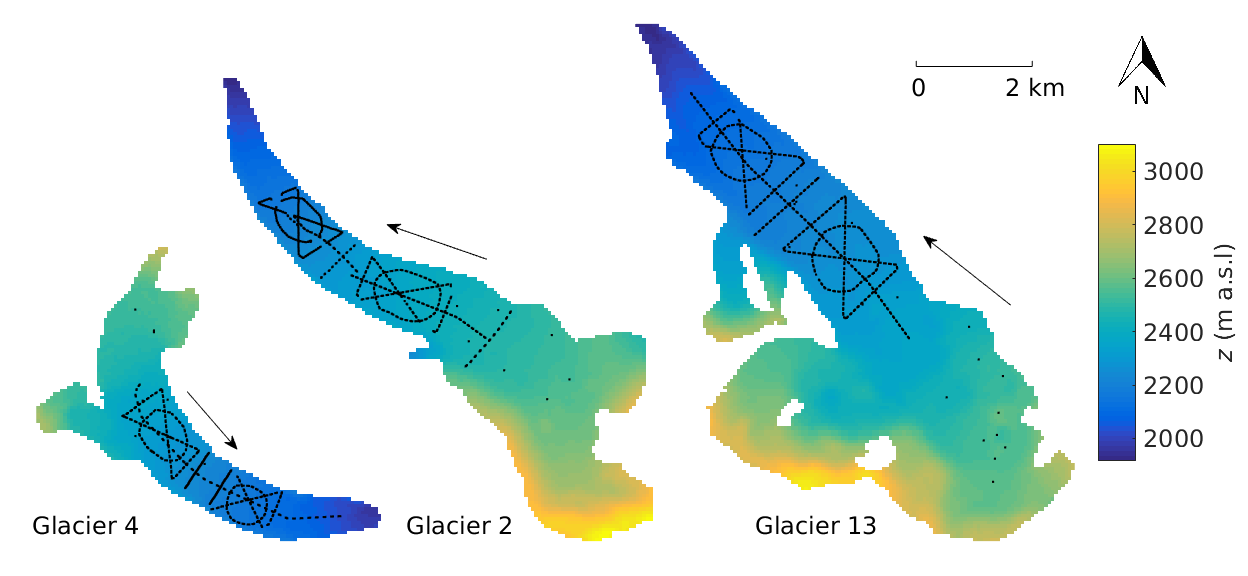
\includegraphics[width = \textwidth]{Map_elevation.png}\\
	\caption{Distributions of elevation ($z$) used in the topographic regressions for the study glaciers. This DEM is derived from a SPOT5 satellite image and has a grid size of 40$\times$40 m. Subsequent topographic parameters were derived from this DEM. \topomap}
	\label{map:elev}
\end{figure}

\begin{figure}[H]
  \makebox[\textwidth][c]{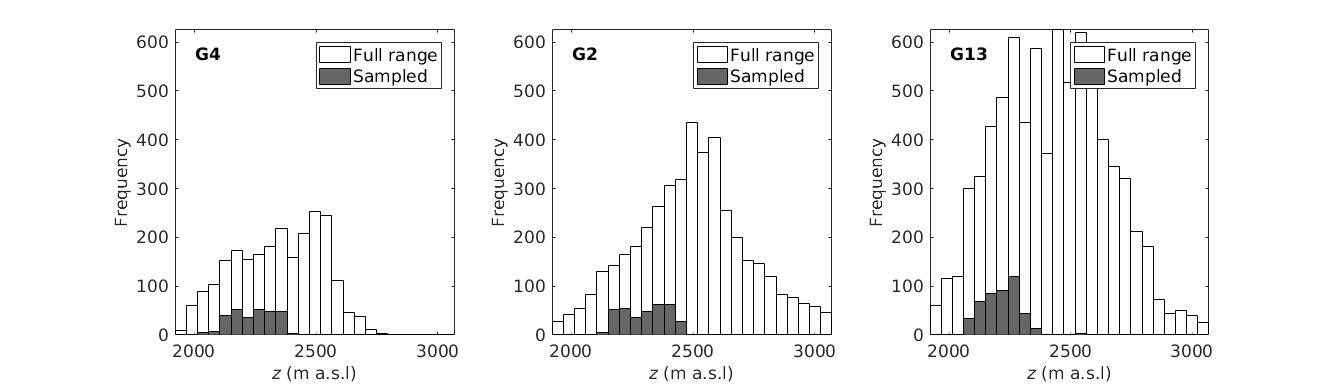
\includegraphics[width=1.2\textwidth]{SampledRangeTopo_elevation.png}}%
	\caption{Histograms of elevation ($z$) sampled (brown) as compared to total range of elevation (blue) of study glaciers.}
	\label{sampledRange:elev}
\end{figure}

\begin{figure}[H]
	\centering
	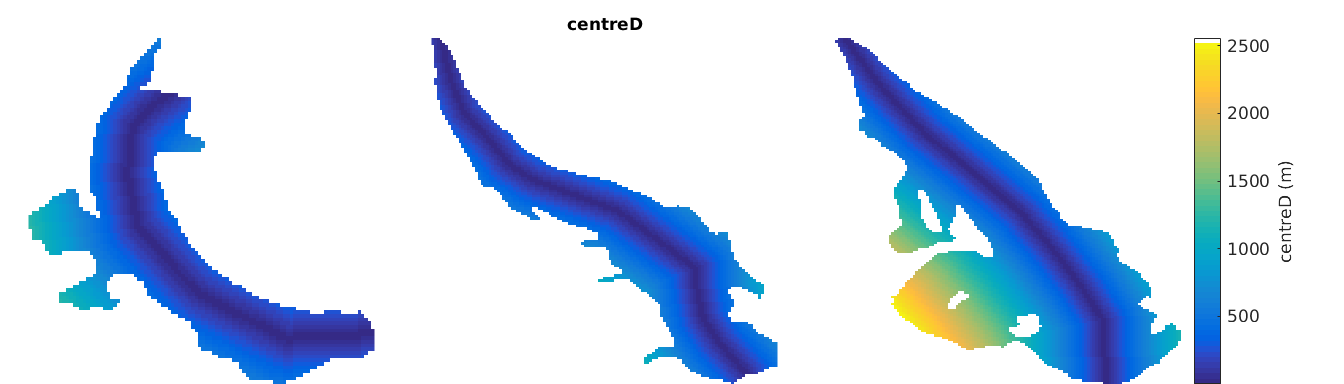
\includegraphics[width=\textwidth]{Map_centreD.png}\\
	\caption{Distributions of distance from centreline ($d_C$) used in the topographic regressions for the study glaciers. Centreline was drawn by hand in QGIS. \topomap}
	\label{map:centreD}
\end{figure}

\begin{figure}[H]
	 \makebox[\textwidth][c]{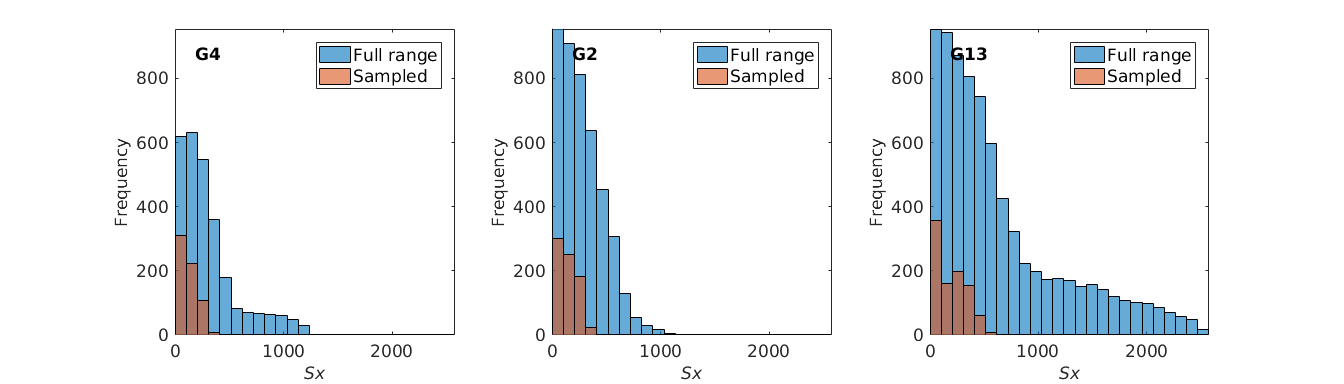
\includegraphics[width=1.2\textwidth]{SampledRangeTopo_centreD.png}}%
	\caption{Histograms of distance from centreline ($d_c$) sampled (brown) as compared to total range (blue) of distance from centreline of study glaciers.}
	\label{sampledRange:centreD}
\end{figure}

\begin{figure}[H]
	\centering
	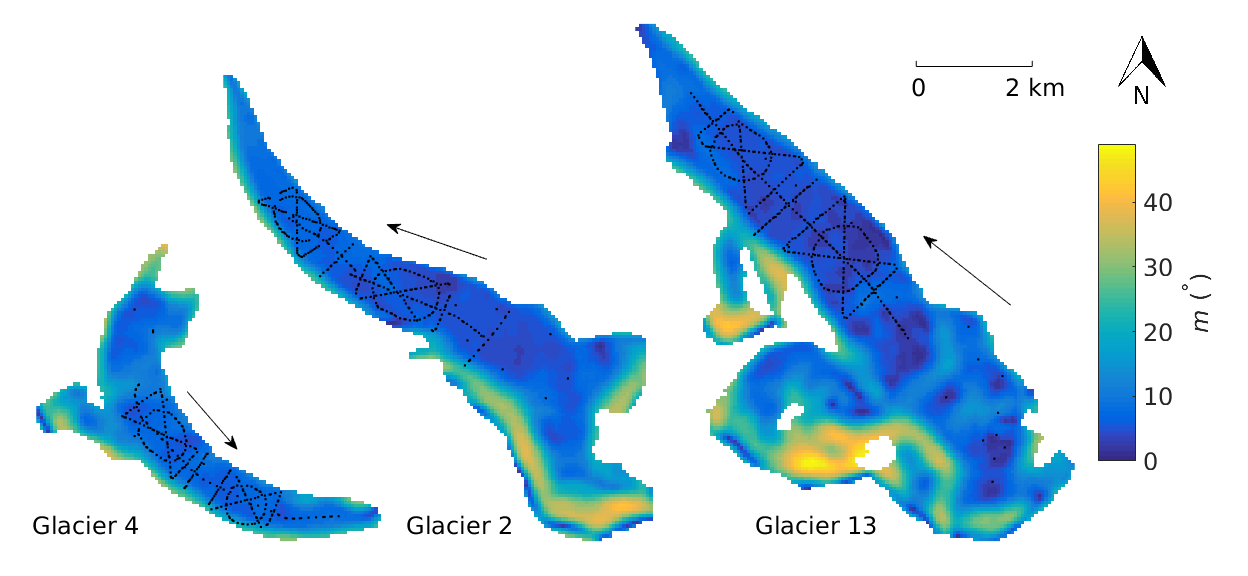
\includegraphics[width=\textwidth]{Map_slope.png}\\
	\caption{Distributions of slope ($m$) used in the topographic regressions for the study glaciers. Values were derived from a SPOT5 satellite derived DEM (grid size of 40$\times$40 m) in QGIS. \topomap}
	\label{map:slope}
\end{figure}

\begin{figure}[H]
	 \makebox[\textwidth][c]{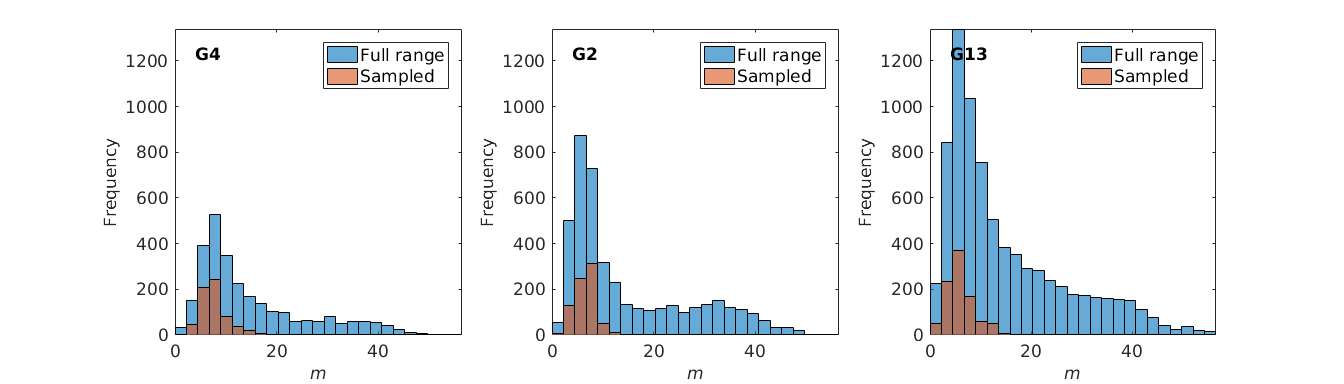
\includegraphics[width=1.2\textwidth]{SampledRangeTopo_slope.png}}%
	\caption{Histograms of slope ($m$) sampled (brown) as compared to total range (blue) of slope of study glaciers.}
	\label{sampledRange:slope}
\end{figure}

\begin{figure}[H]
	\centering
	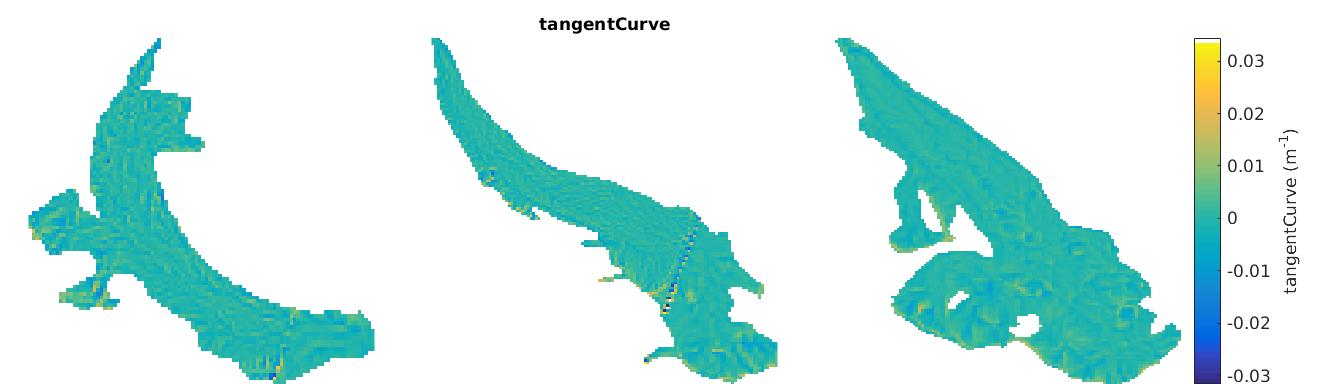
\includegraphics[width=\textwidth]{Map_tangentCurve.png}\\
	\caption{Distributions of tangential curvature ($\kappa_T$) used in the topographic regressions for the study glaciers. Values were derived from a SPOT5 satellite derived DEM (grid size of 40$\times$40 m) in QGIS. Colour axis has been scaled to better resolve values close to zero. \topomap}
	\label{map:tangentC}
\end{figure}

\begin{figure}[H]
	 \makebox[\textwidth][c]{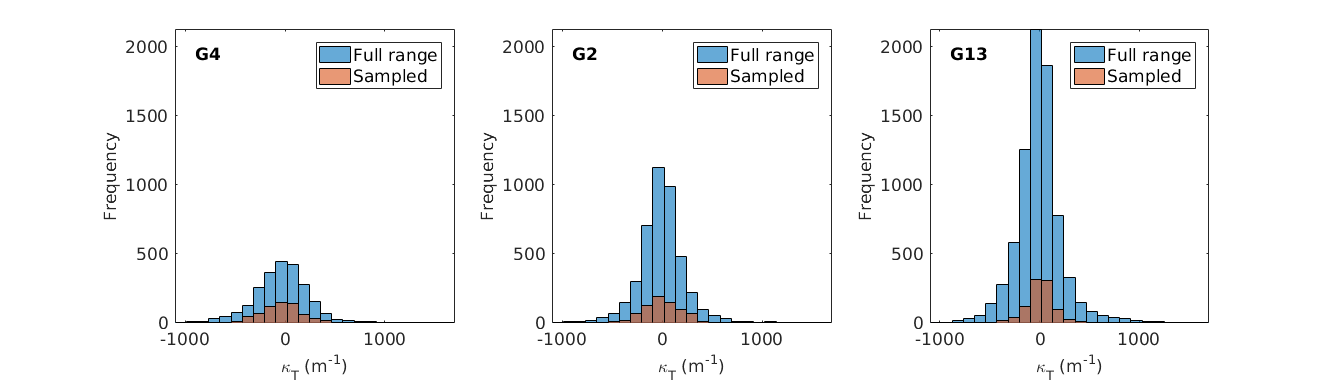
\includegraphics[width=1.2\textwidth]{SampledRangeTopo_tangentCurve.png}}%
	\caption{Histograms of tangential curvature ($\kappa_T$) sampled (brown) as compared to total range (blue) of tangential curvature of study glaciers.}
	\label{sampledRange:tangentC}
\end{figure}

\begin{figure}[H]
	\centering
	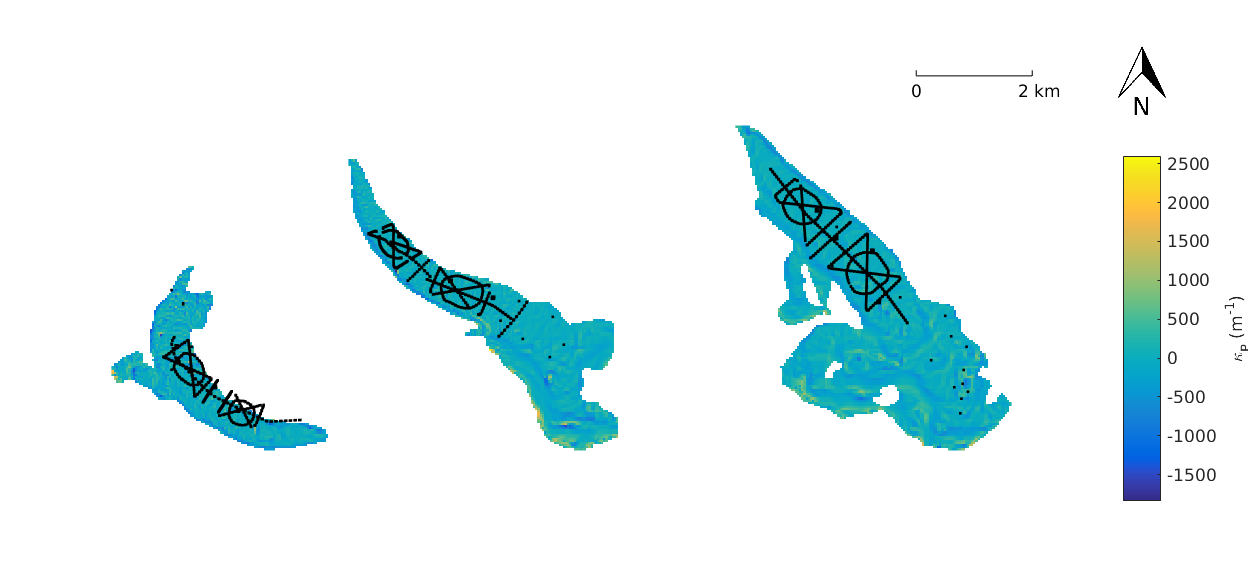
\includegraphics[width=\textwidth]{Map_profileCurve.png}\\
	\caption{Distributions of profile curvature ($\kappa_P$) used in the topographic regressions for the study glaciers. Values were derived from a SPOT5 satellite derived DEM (grid size of 40$\times$40 m) in QGIS. Colour axis has been scaled to better resolve values close to zero. \topomap}
	\label{map:profileC}
\end{figure}

\begin{figure}[H]
	 \makebox[\textwidth][c]{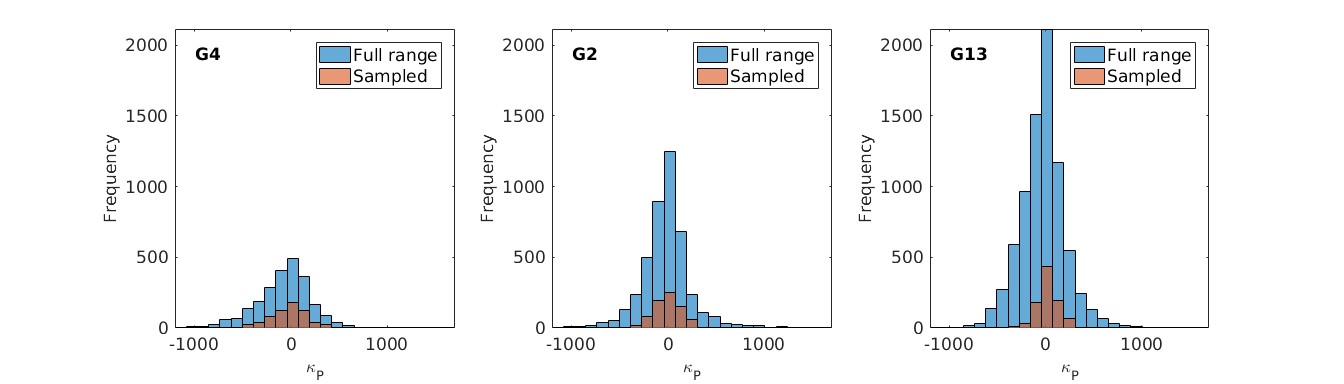
\includegraphics[width=1.2\textwidth]{SampledRangeTopo_profileCurve.png}}%
	\caption{Histograms of profile curvature ($\kappa_P$) sampled (brown) as compared to total range (blue) of profile curvature of study glaciers.}
	\label{sampledRange:profileC}
\end{figure}

\begin{figure}[H]
	\centering
	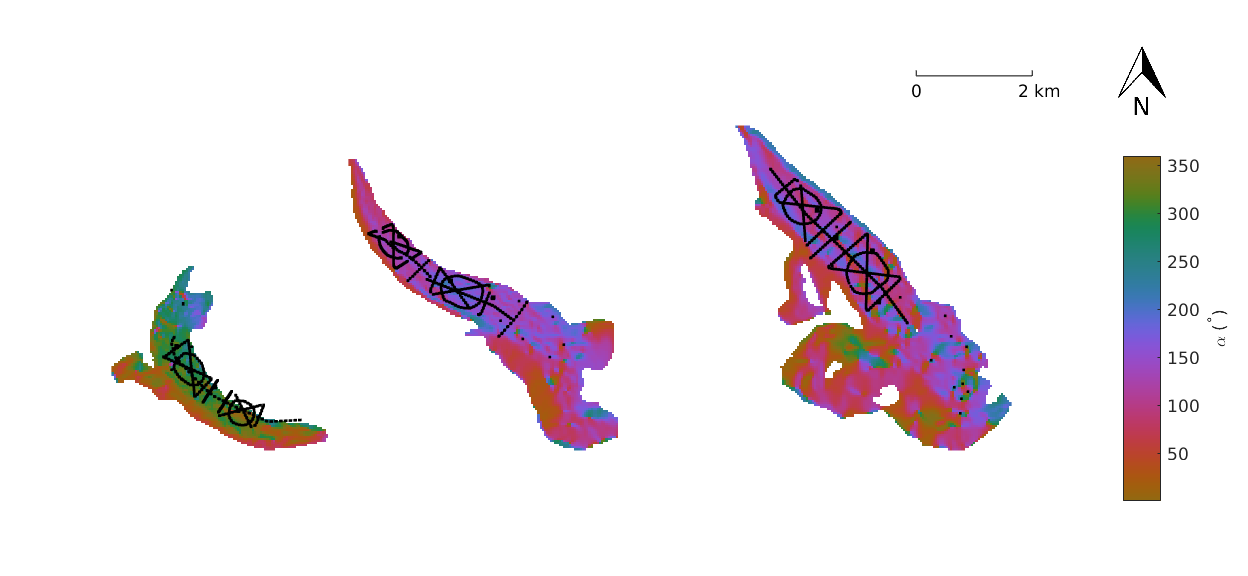
\includegraphics[width=\textwidth]{Map_aspect.png}\\
	\caption{Distributions of aspect ($\alpha$), which indicates the direction that a slope is facing (0${^\circ}$ defined as north), used in the topographic regressions for the study glaciers. \topomap}
	\label{map:aspect}
\end{figure}

\begin{figure}[H]
	 \makebox[\textwidth][c]{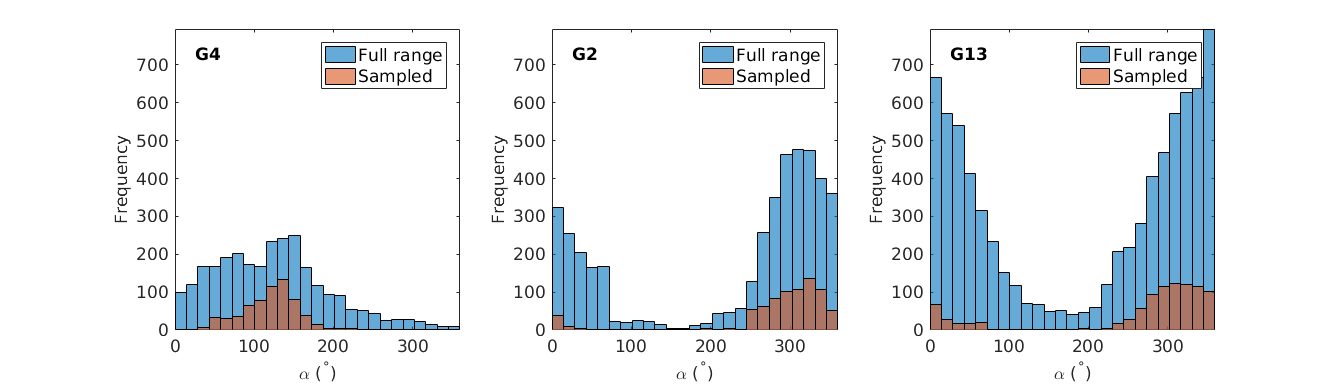
\includegraphics[width=1.2\textwidth]{SampledRangeTopo_aspect.png}}%
	\caption{Histograms of aspect ($\alpha$) sampled (brown) as compared to total range (blue) of aspect of study glaciers.}
	\label{sampledRange:aspect}
\end{figure}

\begin{figure}[H]
	\centering
	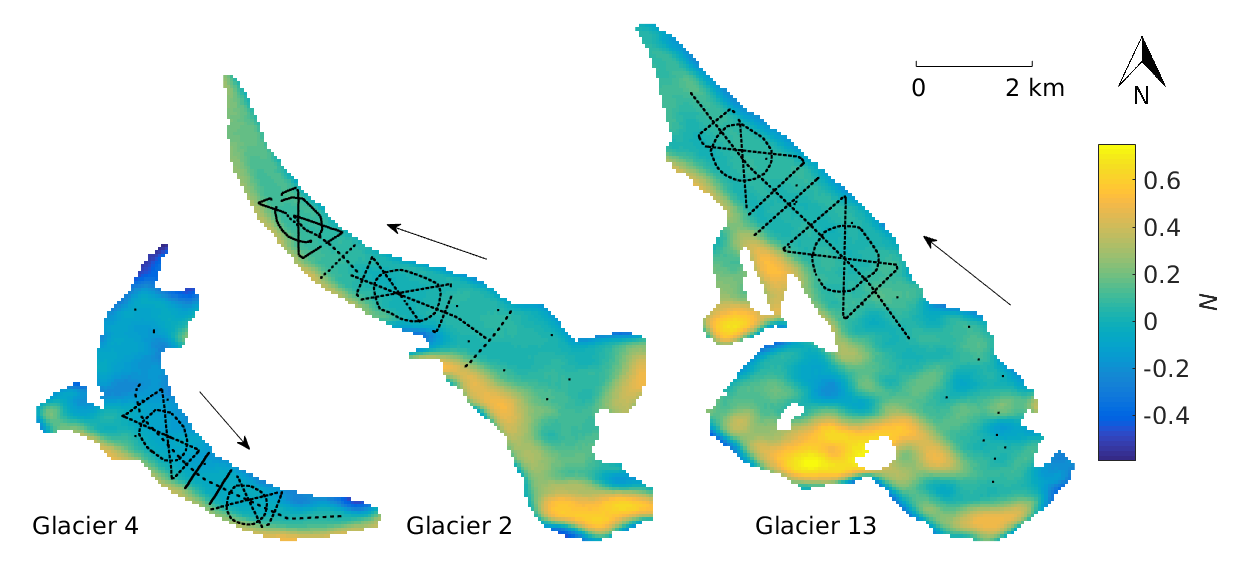
\includegraphics[width=\textwidth]{Map_northness.png}\\
	\caption{Distributions of ``northness'' ($N$) used in the topographic regressions for the study glaciers. ``Northness'' is defined as the product of the cosine of aspect and sine of slope. A value of -1 represents a steep, south facing slope, a value of +1 represents a steep, north facing slope, and flat surfaces yield 0. Values were derived from a SPOT5 satellite derived DEM (grid size of 40$\times$40 m) in QGIS. \topomap}
	\label{map:northness}
\end{figure}

\begin{figure}[H]
	 \makebox[\textwidth][c]{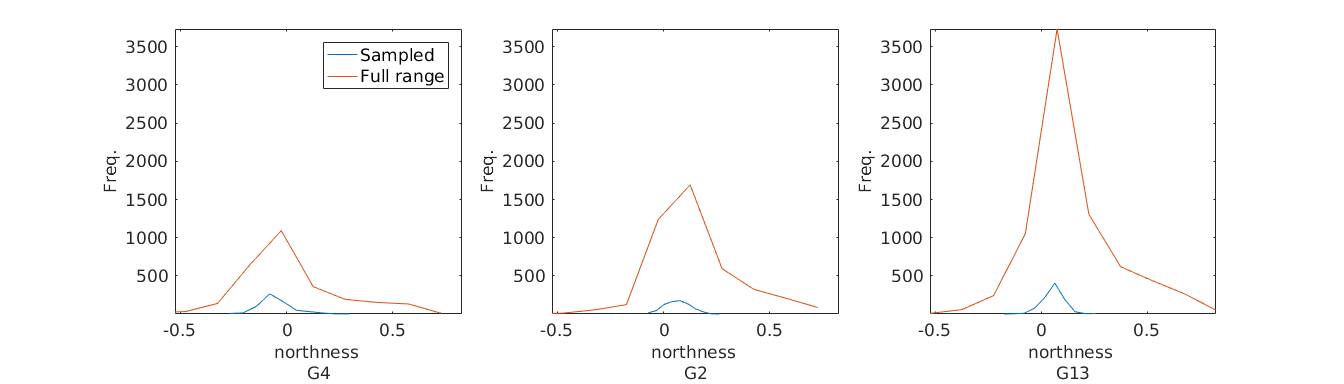
\includegraphics[width=1.2\textwidth]{SampledRangeTopo_northness.png}}%
	\caption{Histograms of ``northness'' ($N$) sampled (brown) as compared to total range (blue) of ``northness'' of study glaciers.}
	\label{sampledRange:northness}
\end{figure}

\begin{figure}[H]
	\centering
	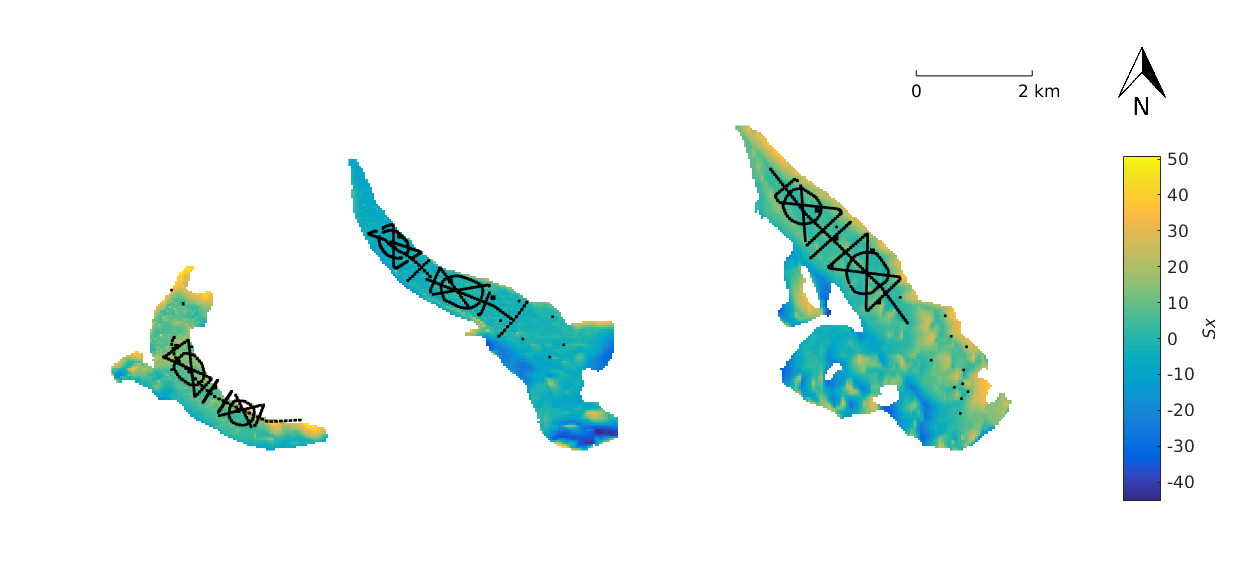
\includegraphics[width=\textwidth]{Map_Sx.png}\\
	\caption{Distributions of $Sx$, which is a wind redistribution parameter, used in the topographic regressions for the study glaciers. See section \ref{sec:topoCalc} and the original paper by \cite{Winstral2002} for more details on calculation. See Table \ref{tab:Sxparams} for values of best correlated azimuth and maximum search distance for each glacier. \topomap}
	\label{map:Sx}
\end{figure}

\begin{figure}[H]
	 \makebox[\textwidth][c]{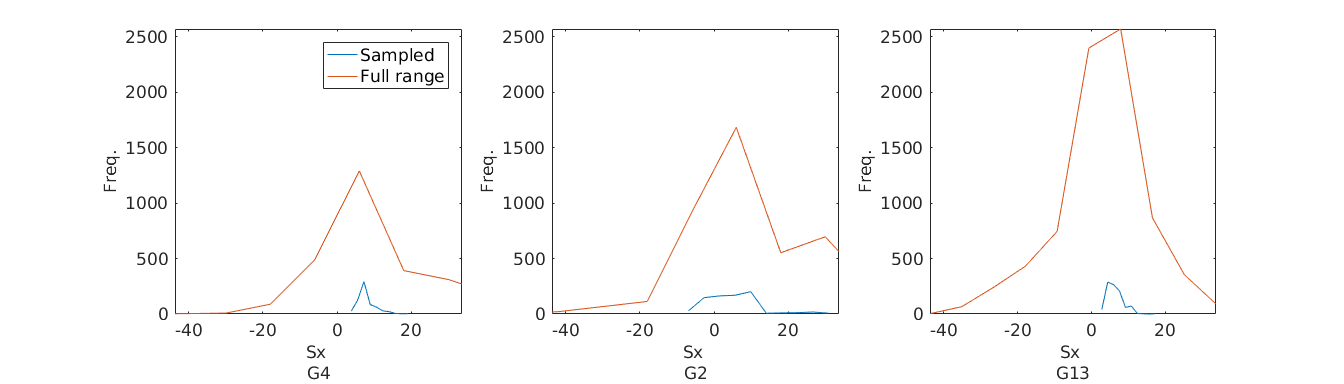
\includegraphics[width=1.2\textwidth]{SampledRangeTopo_Sx.png}}%
	\caption{Histograms of $Sx$ sampled (brown) as compared to total range (blue) of $Sx$ of study glaciers.}
	\label{sampledRange:Sx}
\end{figure}


%%%%%%%%%%%%%%%%%%%%%%%%%%%%%%%%%%%%%%%%%%%%%%%%%%
\section{Linear Regressions}
\label{sec:linearregression}

\subsection{Background}
Relating snow accumulation and terrain parameters to better predict accumulation within a basin has been employed for decades \citep[e.g.][]{Woo1978, Molotch2005, McGrath2015}. The most common type of relation between topographic parameters and accumulation is a linear regression, where the observed snow water equivalent (SWE) is related to a linear combination of topographic parameters at each measurement location. 

A linear regression takes the form
\begin{equation}
\vector{y} = \vector{X} \bm{\beta} + \bm{\varepsilon},
\end{equation}
where the matrix $\vector{X}$ contains the set of independent regressors $\vector{x}_i$ used to explain the dependant variable $\vector{y}$ \citep[e.g.][]{Davis1986}. The regression coefficient for each regressor is given by $\bm{\beta}$ and the error of the system is given by $\bm{\varepsilon}$. Applied to this study, the matrix of independent regressors ($\vector{X}$) contains the topographic parameters at the sampling locations, the dependent variable $\vector{y}$ contains the observed SWE, and the $\bm{\beta}$ values are determined using a fitting model. While there are many types of fitting models, the ones employed in this study are multiple linear regression (MLR) and Bayesian model averaging (BMA).

To prevent over fitting of the data, regressions are calculated using cross validation. This means that for each regression, a randomly selected portion of the data is used to estimate regression coefficients and the coefficients are used to predict values that correspond to the remaining data \citep{Kohavi1995}. The root mean squared error (RMSE) between the estimated and observed data is then calculated. This process was repeated 1000 times and the regression coefficients that resulted in the lowest RMSE are then chosen for that model. 

In this study, regressions for all possible combinations of topographic parameters are calculated. The total number of models is $2^n$ , where $n$ is the number of topographic parameters. Eight topographic parameters are used, resulting in $2^8 = 256$ models. Model averaging is then used to determine the final regression coefficients. Model averaging is described in more details for multiple linear regressions (MLRs) in Section \ref{sec:MLR} and for Bayesian Model Averaging (BMA) in Section \ref{sec:BMS}.

Once $\bm{\beta}$ values have been estimated, they can then be used to predict values of the dependent variable in other locations where regressors are known \citep{Davis1986}. For each grid cell, known values of topographic parameters can be multiplied by their respective $\bm{\beta}$ coefficients and added together to obtain the modelled or predicted value of SWE.

\subsection{Snow density estimation methods}

In this study, snow density was not measured at every location where snow depth was measured. Therefore, snow density values need to be estimated at snow depth measurement locations in order to estimate observed SWE values. There are a number of different methods for interpolating between snow density measurement locations. Four methods were chosen for this study and include (1) using a constant value, the mean of all observed snow density values, for all measurement locations, (2) using a constant value (mean) for each glacier, (3) using a linear regression of elevation and snow density to interpolate for each glacier, and (4) taking an inverse-distance weighted mean of density observations. As discussed in Section ??, the snowpit-derived densities and Federal Sampler-derived densities are inconsistent so these two data set are kept separate for the analysis. In total there are eight different methods for estimating density, as summarized in Table \ref{tab:densityOptions}.

\begin{table}[H]
\centering
\caption{Description of density interpolation methods used to calculate SWE used in the topographic regression. Abbreviations with `S' used snowpit-derived densities and abbrviations with an `F' used Federal Sampler-derived densities.}
\label{tab:densityOptions}
\begin{tabular}{c|cc|c}
 & \multicolumn{2}{c|}{\textbf{Source of snow density}} &  \\
 & \textit{Snowpit} & \begin{tabular}[c|]{c} \textit{Federal}\\  \textit{Sampler}\end{tabular} & \multirow{-2}{*}{\textbf{\begin{tabular}[|c]{c}Estimation\\ method\end{tabular}}} \\   \hline

S1 & $\blacksquare$ &  &  \\
 
F1 &  & $\blacksquare$ & \multirow{-2}{*}{\begin{tabular}[c]{@{}c@{}}Mean of all glaciers \end{tabular}} \\  \hline
S2 & $\blacksquare$ &  &  \\
F2 &  & $\blacksquare$ & \multirow{-2}{*}{Glacier mean} \\ \hline
 
S3 & $\blacksquare$ &  &  \\
 
F3 &  & $\blacksquare$ & \multirow{-2}{*}{\begin{tabular}[c]{@{}c@{}}Linear regression of elevation and\\ density for each glacier \end{tabular}} \\ \hline
S4 & $\blacksquare$ &  &  \\
F4 &  & $\blacksquare$ & \multirow{-2}{*}{\begin{tabular}[c]{@{}c@{}}Inverse distance\\ weighted mean\end{tabular}}
\end{tabular}
\end{table}


\subsection{Multiple Linear Regression (MLR)}
\label{sec:MLR}

\subsubsection{Background}

Perhaps the most basic and well used method for relating SWE and topographic parameters is a multiple linear regression (MLR) \citep[e.g.][]{Cohen2013}. The best fit line of one type of MLR is the one described by coefficients that minimize the sum of squares of the vertical deviations of each data point ($Y_i$) from the estimated value according to the equation ($\hat{Y}_i$) \citep{Davis1986}
\begin{equation}
\sum^n_{i=1}(\hat{Y}_i-Y_i)^2 = \mathrm{minimum}.
\end{equation}
Note that if a point falls on the line then the deviation is zero and  the positive and negative deviations from the line do not cancel because the values are first squared and then summed. The residuals are simply the differences between the estimated and observed data values. To prevent over fitting of the data, cross validation is done for each MLR, as described in Section \ref{sec:linearregression}.

In this study, there are $2^8$ models that encompass all possible linear combinations of topographic parameters. There is no reason to favour any of the models so a weighted sum of all models is used to estimate regression coefficients. The Bayesian information criterion (BIC) value is used to assess the relative predictive success of each model. 

A BIC value is found according to
\begin{equation}
\textrm{BIC} = -2 \ln L(\hat\theta_k  | y) + k \ln(n),
\end{equation}
where the values of $\hat \theta_k$, which are the model parameters, maximize the likelihood function for data $y$ \citep{Burnham2004}. The likelihood function, $ L(\hat\theta_k  | y)$, is the probability of the model parameters occurring given the data. The number of data points is $n$ and the number of regressors is $k$. BIC values are used to assess the relative predictive success of models while penalizing for overfitting of data. While the absolute BIC value is meaningless, models can be selected or averaged using the relative BIC values, with lower values indicating a better model \citep{Burnham2004}. 

The BIC value for each model ($BIC_i$) is used to determine the normalized weight of each model ($w_i$) relative to the best model (lowest BIC value indicated by $BIC_{\min}$) as defined by the equation \citep{Burnham2004}
\begin{equation}
w_i = \frac{e^{-0.5(BIC_i-BIC_{\min})}}{\Sigma_{i=1}^R e^{-0.5(BIC_i-BIC_{\min})}}.
\label{eq:BIC}
\end{equation}
Parameters not included in a particular model are assigned coefficients of zero. The sum of the weighted coefficients gives the final $\bm{\beta}$ values.

\subsubsection{Computational Methods}
\label{sec:MLRMethods}

The MLR was completed with the following steps (executed using the function 'MLRcalval.m'):
\begin{enumerate}
\item The topographic parameters are imported to Matlab using the script `Import\_Topo.m'.

\item The \texttt{topo\_sampled} structure for one glacier as well as the \texttt{SWE} structure is passed into the function.

\item A set of initializations is completed. This includes 1) creating a logical matrix to choose all linear combinations of topographic parameters, 2) selecting the number of runs, 3) creating a matrix of random numbers for selecting data points in the cross validation procedure, 4) initializing matrices, and 5) converting the input structure to a table.

\item For each linear combination of topographic parameters, 1000 runs of a cross validation MLR are then executed. Two-thirds of the total data is randomly selected \citep{Kohavi1995} to use for calculating the regression (using the function \texttt{regress()} which is a basic regression function with fast execution). The MLR equation is used to predict the SWE using the remaining one-third of the topographic parameters. The root-mean-squared error (RMSE) between the predicted and observed SWE values is then calculated and the set fo regression coefficients that produce the lowest RMSE are then chosen for that combination of topographic parameters. The function \texttt{fitlm()} is then used to calculate the MLR from the set of data that gave the lowest RMSE. This function is slower but calculates a number of additional values that characterize the fit of the model. One of these values is the Bayesian information criterion (BIC), which allows for model selection among a finite set of models \citep{Burnham2004}. The BIC from the best model for each combination of topographic parameters is saved.

\item A weighted sum of all models found using linear combinations of topographic parameters was then found. The BIC values for each model (BIC$_i$) were used to determine the normalized weight of each model ($w_i$) relative to the best model (lowest BIC value BIC$_{min}$) according to Eq. \ref{eq:BIC}.

\item The percent variance ($var_\%$) explained by each parameter was calculated using the equation $var_\% = \frac{SSr}{SSt}\times 100$, where $SSr$ is the sum of squares of the residual (fitted topographic parameters) and $SSt$ is the total sum of squares (SWE observations). The final coefficients and the percent variance explained by each one can be found in the \texttt{coeffs\_final} table within the function and in the \texttt{mlr} structure when run for all density options and glaciers in the main script `TopoRegression.m'.

\item The residuals of the fit have also been calculated as a separate variable that can be returned when the function is called. The residual is calculated as the difference between the estimated SWE value and observed value. 
\end{enumerate}


\subsubsection{Results}

\begin{wraptable}{R}{11cm}
\centering
\caption{MLR coefficients for topographic regression between measured SWE (found using inverse-distance weighted snowpit-derived densities) and standardized topographic parameters. \params  Since parameters are standardized, the magnitude of the coefficients is representative of their importance in predicting SWE. The root-mean-squared error (RMSE) between modelled SWE using those coefficients and observed SWE is also given.}
\label{tab:MLRcoeff}
\begin{tabular}{ccrrr}
 Parameter & Units & \textbf{Glacier 4} & \textbf{Glacier 2} & \textbf{Glacier 13} \\ \hline
d$_C$ 			&m&  \textless-0.001		& 0.019 					& 0.013 \\
$z$ 				&m a.s.l & 0.009 						& 0.098					& 0.047 \\
$\alpha$ 		& ---& 0.001 						& -0.002 					& -0.004 \\
$m$ 			& ---& -0.021 						& 0.013					 &  \textless-0.001 \\
$N$ 				& ---& \textless-0.001		  	& 0.001 					& 0.002 \\
$\kappa_P$ &m$^{-1}$& -0.002 						& \textless0.001 		& -0.001 \\
$\kappa_T$&m$^{-1}$ & \textless-0.001 		& 0.005 					& -0.001 \\
$Sx$ 			& ---& -0.045 						& 0.041 					&0.012 \\
Intercept 		&& 0.625 						& 0.267 					& 0.241 \\ \hline
RMSE 			&& 0.147						& 0.104 					& 0.089
\end{tabular}
\end{wraptable}


\begin{sidewaystable}
\centering
\caption{Topographic regression coefficients of standardized parameters determined using MLR. See Table \ref{tab:densityOptions} for description of density options.}
\label{tab:MLRcoeffFull}
\begin{tabular}{ccrrrrrrrr}
 & \textbf{\begin{tabular}[c]{@{}c@{}}Topographic\\ Parameter\end{tabular}} & \textbf{S1} & \textbf{F1} & \textbf{S2} & \textbf{F2} & \textbf{S3} & \textbf{F3} & \textbf{S4} & \textbf{F4} \\ \hline \hline
 
 & $d_C$ & $-$0.003 & $-$0.001 & $-$0.001 & $-$0.001 & $-$0.002 & $-$0.002 & $-$0.001 & $-$0.005 \\
 
 & $z$ & 0.008 & 0.014 & 0.004 & 0.022 & 0.028 & 0.000 & 0.009 & 0.002 \\
 
 & $\alpha$ & 0.001 & 0.002 & 0.001 & 0.001 & 0.003 & 0.000 & 0.001 & 0.000 \\
 
 & $m$ & $-$0.020 & $-$0.014 & $-$0.025 & $-$0.012 & $-$0.009 & $-$0.020 & $-$0.021 & $-$0.023 \\
 
 & $N$ & $-$0.001 & $-$0.004 & 0.000 & $-$0.006 & $-$0.004 & $-$0.001 & 0.000 & 0.000 \\
 
 & $\kappa_P$ & $-$0.001 & $-$0.003 & 0.000 & $-$0.004 & $-$0.004 & $-$0.001 & $-$0.002 & $-$0.001 \\
 
 & $\kappa_T$ & 0.000 & 0.000 & 0.000 & 0.000 & 0.000 & 0.000 & 0.000 & 0.000 \\
 
 & $Sx$ & $-$0.040 & $-$0.044 & $-$0.046 & $-$0.053 & $-$0.048 & $-$0.051 & $-$0.045 & $-$0.038 \\
 
 & Intercept & 0.619 & 0.581 & 0.627 & 0.646 & 0.630 & 0.648 & 0.625 & 0.639 \\
 
\multirow{-10}{*}{Glacier 4} & RMSE & 0.146 & 0.135 & 0.149 & 0.151 & 0.148 & 0.152 & 0.147 & 0.150 \\ \hline
 & $d_C$ & 0.020 & 0.020 & 0.020 & 0.018 & 0.020 & 0.017 & 0.019 & 0.012 \\
 & $z$ & 0.113 & 0.100 & 0.109 & 0.089 & 0.090 & 0.107 & 0.098 & 0.110 \\
 & $\alpha$ & $-$0.004 & $-$0.001 & $-$0.007 & $-$0.001 & $-$0.001 & $-$0.001 & $-$0.001 & $-$0.010 \\
 & $m$ & 0.019 & 0.018 & 0.016 & 0.011 & 0.007 & 0.012 & 0.013 & 0.011 \\
 & $N$ & 0.002 & 0.000 & 0.004 & 0.001 & 0.000 & 0.001 & 0.001 & 0.005 \\
 & $\kappa_P$ & 0.000 & 0.000 & 0.000 & 0.000 & 0.000 & 0.000 & 0.000 & 0.001 \\
 & $\kappa_T$ & 0.001 & 0.002 & 0.004 & 0.000 & 0.004 & 0.002 & 0.005 & 0.002 \\
 & $Sx$ & 0.041 & 0.039 & 0.040 & 0.032 & 0.040 & 0.033 & 0.041 & 0.035 \\
 & Intercept & 0.268 & 0.250 & 0.263 & 0.225 & 0.256 & 0.225 & 0.267 & 0.229 \\
\multirow{-10}{*}{Glacier 2} & RMSE & 0.104 & 0.097 & 0.101 & 0.087 & 0.102 & 0.087 & 0.104 & 0.088 \\ \hline
 
 & $d_C$ & 0.013 & 0.009 & 0.009 & 0.009 & 0.013 & 0.010 & 0.013 & 0.009 \\
 
 & $z$ & 0.049 & 0.047 & 0.054 & 0.047 & 0.044 & 0.050 & 0.047 & 0.047 \\
 
 & $\alpha$ & $-$0.002 & $-$0.002 & $-$0.003 & $-$0.003 & $-$0.005 & $-$0.001 & $-$0.004 & $-$0.002 \\
 
 & $m$ & $-$0.002 & $-$0.001 & $-$0.001 & 0.000 & $-$0.001 & $-$0.001 & 0.000 & 0.000 \\
 
 & $N$ & 0.003 & 0.002 & 0.001 & 0.006 & 0.002 & 0.001 & 0.002 & 0.001 \\
 
 & $\kappa_P$ & 0.000 & 0.000 & 0.000 & 0.000 & 0.000 & 0.000 & $-$0.001 & 0.000 \\
 
 & $\kappa_T$ & 0.000 & 0.000 & 0.000 & 0.000 & $-$0.001 & 0.000 & $-$0.001 & $-$0.001 \\
 
 & $Sx$ & 0.011 & 0.011 & 0.011 & 0.006 & 0.009 & 0.012 & 0.012 & 0.010 \\
 
 & Intercept & 0.231 & 0.213 & 0.235 & 0.214 & 0.246 & 0.202 & 0.241 & 0.207 \\
 
\multirow{-10}{*}{Glacier 13} & RMSE & 0.085 & 0.080 & 0.087 & 0.079 & 0.092 & 0.074 & 0.089 & 0.077

\end{tabular}
\end{sidewaystable}

The coefficients determined using MLR for density S4 can be seen in Table \ref{tab:MLRcoeff} and can be used to examine the relative importance of topographic parameters in the regression. These coefficients were found for standardized values of topographic parameters so their magnitude is indicative of their importance in predicting SWE. Table \ref{tab:MLRcoeffFull} shows coefficient values for all density options. The range of percent variance explained by each variable (from all density options) can be seen in Figure \ref{fig:MLRPercentVar_densityOptions}. The fit between modelled SWE and observed SWE for each glacier for density Option 7 can be seen in Figure \ref{fig:MLRfit_opt8} and the fit for all density options in Figure \ref{fig:MLRfit_allLines}. The distribution of residuals in then plotted in Figure \ref{fig:MLRresiduals_all}. A map of the predicted values of SWE over the entire glacier using density option 7 can be seen in Figure \ref{fig:MLRmodelledSWE} with basic summary statistics found in Table \ref{tab:MLRsweMinMax}. Modelled SWE using all density options is shown in Figure \ref{fig:allMLRmodelled}. A map of the difference between maximum and minimum modelled SWE values is shown in Figure \ref{fig:MLR_SWEdiffMap}.

For Glacier 4, the largest coefficients are $Sx$ and slope ($m$), which are an order of magnitude larger than the remaining coefficients. Both coefficients are negative, which indicates less snow in `sheltered' areas and less on steeper slopes. These coefficients account for the largest percentage of variance explained, although this percentage is small ($\sim$7\% and $\sim$1\%, respectively). Overall, the modelled winter balance for Glacier 4 is very poorly explained by the topographic parameters, which results in no correlation between modelled and observed SWE (R$^2_{avg}=0.06$) and a comparatively high RMSE value. The modelled values of SWE are largely determined by the intercept value. The map of predicted SWE for the entire glacier shows a relatively uniform SWE distribution over Glacier 4, likely due to the large influence of the intercept on the regression. Areas with steep slopes and high $Sx$ values (sheltered), especially in the accumulation area, have the lowest values of SWE. This regression indicates that the wind effects play a significant role in snow distribution but since the valley in which the glacier sits is steep walled and curved, perhaps having a single cardinal direction for wind is inappropriate. Examining $Sx$ values that assume wind moving up or down glacier and changing direction to follow the valley could allow the $Sx$ parameter to explain more of the variance. 

\begin{wraptable}{l}{8.5cm}
\centering
\caption{Basic summary statistics of modelled SWE using coefficients found using MLR. Values are for coefficients determined using SWE with inverse distance weighted snowpit densities. }
\label{tab:MLRsweMinMax}
\begin{tabular}{lccc}
\multicolumn{1}{l}{} & \multicolumn{3}{c}{\textbf{Modelled SWE (m w.e.)}} \\
                     & Mean          & Minimum          & Maximum         \\ \hline
Glacier 4            & 0.58          & 0.10             & 0.85            \\
Glacier 2            & 0.55          & $-$0.23            & 1.76            \\
Glacier 13           & 0.41          & 0.03             & 0.90           
\end{tabular}
\end{wraptable} 

For Glacier 2, the largest coefficient (by an order of magnitude) is elevation. This coefficient is positive, which means that SWE will increase with elevation. Elevation explains the largest amount of variance ($\sim$45\%) and this is consistent for all density options. $Sx$ and distance from centreline are also significant coefficients in the MLR, explaining $\sim$6\% and $\sim$1\% of the variance, respectively.  Overall, the modelled winter balance is a good estimation of observed SWE (R$^2_{avg}=0.62$) although it tends to underestimate the amount of accumulation. The map of modelled SWE shows the strong dependence on elevation since the values closely resemble the elevation map (Figure \ref{map:elev}). The range of predicted SWE is largest for Glacier 2 and it also has the highest SWE (1.76 m w.e) and the lowest SWE ($-$0.23 m w.e.) values. Both extremes are perhaps unexpected on this glacier and are likely an artefact from extrapolating from the regression, which largely depends on elevation. The southwest region of the accumulation area that has the area of high accumulation is a result of the high elevation and $Sx$ values. The negative values of SWE at the terminus are a result of the low elevation, as the $Sx$ values are close to zero there. 

For Glacier 13, the largest coefficient is elevation with distance from centreline and $Sx$ also of the same order of magnitude. All three coefficients are positive, which means that cells at higher elevation, closer to the margins, and more sheltered had higher amounts of SWE. Elevation explains the majority of the variance (24\%), while distance from centreline and $Sx$ explain far less ($\sim$1\% each).  Overall, the MLR modelled winter balance is poorly related to observed SWE (R$^2_{avg}=0.35$) and tends to underestimate the amount of accumulation. The map of modelled SWE displays an increase with elevation, although it is not strong considering the large range of elevation on this glacier.

Qualitatively, there is little variation in the fit between modelled and observed winter balance between the various density options for all glaciers and the residuals display a similar distribution between the density options.The percent variance explained by each parameter also varies little between different density options. 

The effect of density values on the percent variance explained by each topographic parameters in the MLR is shown in Figure \ref{fig:MLRPercentVar_densityOptions}. The range of percent variance explained by elevation is large for both Glacier 2 and 13 but it does not affect the importance of elevation relative to the other parameters. For these two MLR coefficients, the choice of density interpolation has a large effect on the ability of the model to explain variance in SWE. Using inverse distance weighted, Federal Sampler derived density resulted in the highest percent variance explained (54\%). Since the Federal Sampler derived densities are correlated with snow depth, which is correlated with elevation, it is likely that these density values amplify the elevation component of the regression. The range of percent variance explained for all other parameters is small so the MLR coefficients for these parameters are insensitive to the choice of density interpolation. The values for aspect, ``northness'', and both curvatures are essentially zero. 


\begin{figure}[H]
    \centering
    \begin{subfigure}[b]{\textwidth}
        \makebox[\textwidth][c]{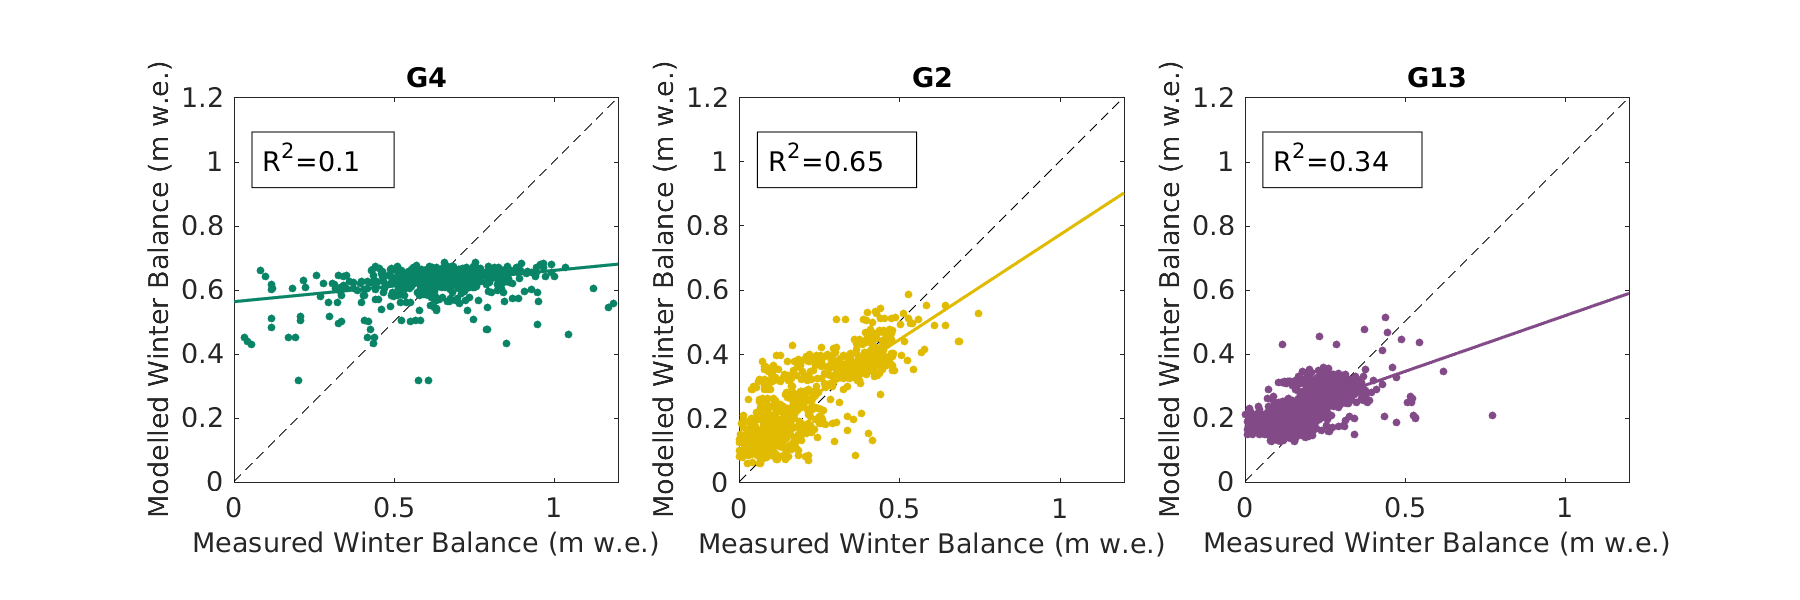
\includegraphics[width=1.2\textwidth]{MLRfit_opt8.png}}
	\label{fig:MLRfit_opt8}
    \end{subfigure}
    
    \begin{subfigure}[b]{\textwidth}
       \makebox[\textwidth][c]{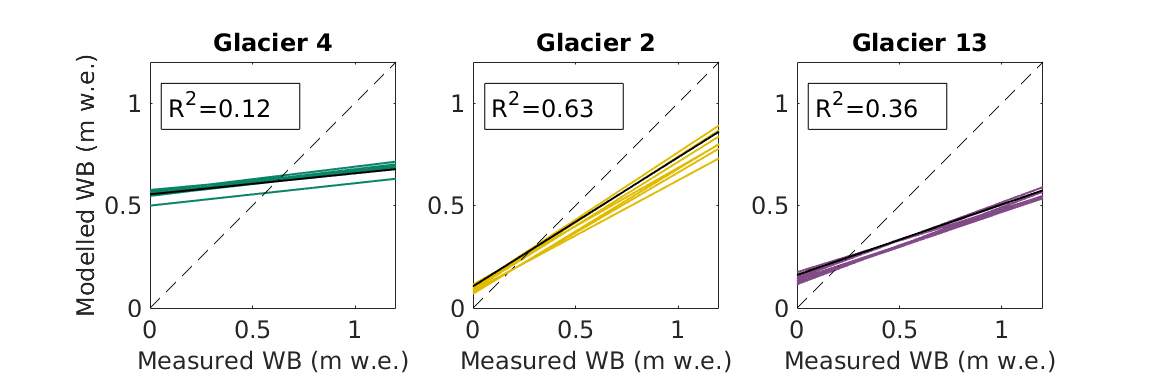
\includegraphics[width=1.2\textwidth]{MLRfit_allLines.png}}
	\label{fig:MLRfit_allLines}
    \end{subfigure}

    \caption{Top panel shows comparison of estimated (MLR) and observed (original) snow water equivalent (SWE) for three study glaciers. The SWE values were calculated using inverse-distance weighted snowpit densities (S4). Bottom panel shows plots of all linear fits between estimated and observed SWE using eight options for calculating density. Mean R$^2$ value is shown for each sub-plot and a reference 1:1 line is also provided. Black line highlights the S4 option from the top panel. See Figure \ref{fig:allMLRmodelled} for a plot of all estimated SWE values.}
\end{figure}


\begin{figure}[H]
	\makebox[\textwidth][c]{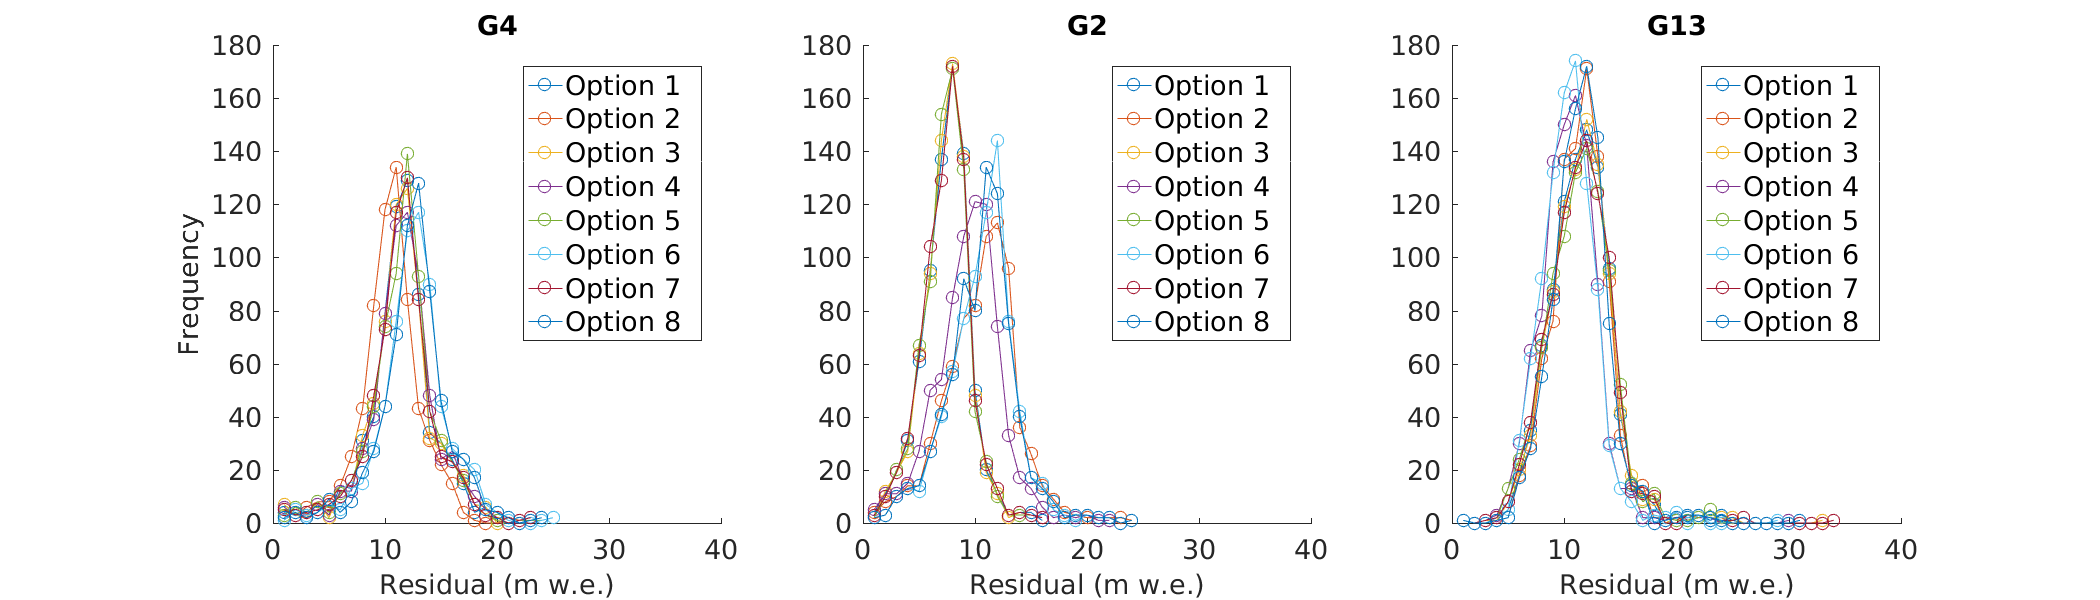
\includegraphics[width=1.2\textwidth]{MLRresiduals_all.png}}%
	\caption{Residuals of SWE predicted using MLR for all options of estimating density.}
	\label{fig:MLRresiduals_all}
\end{figure}
\begin{figure}[H]
	\centering
	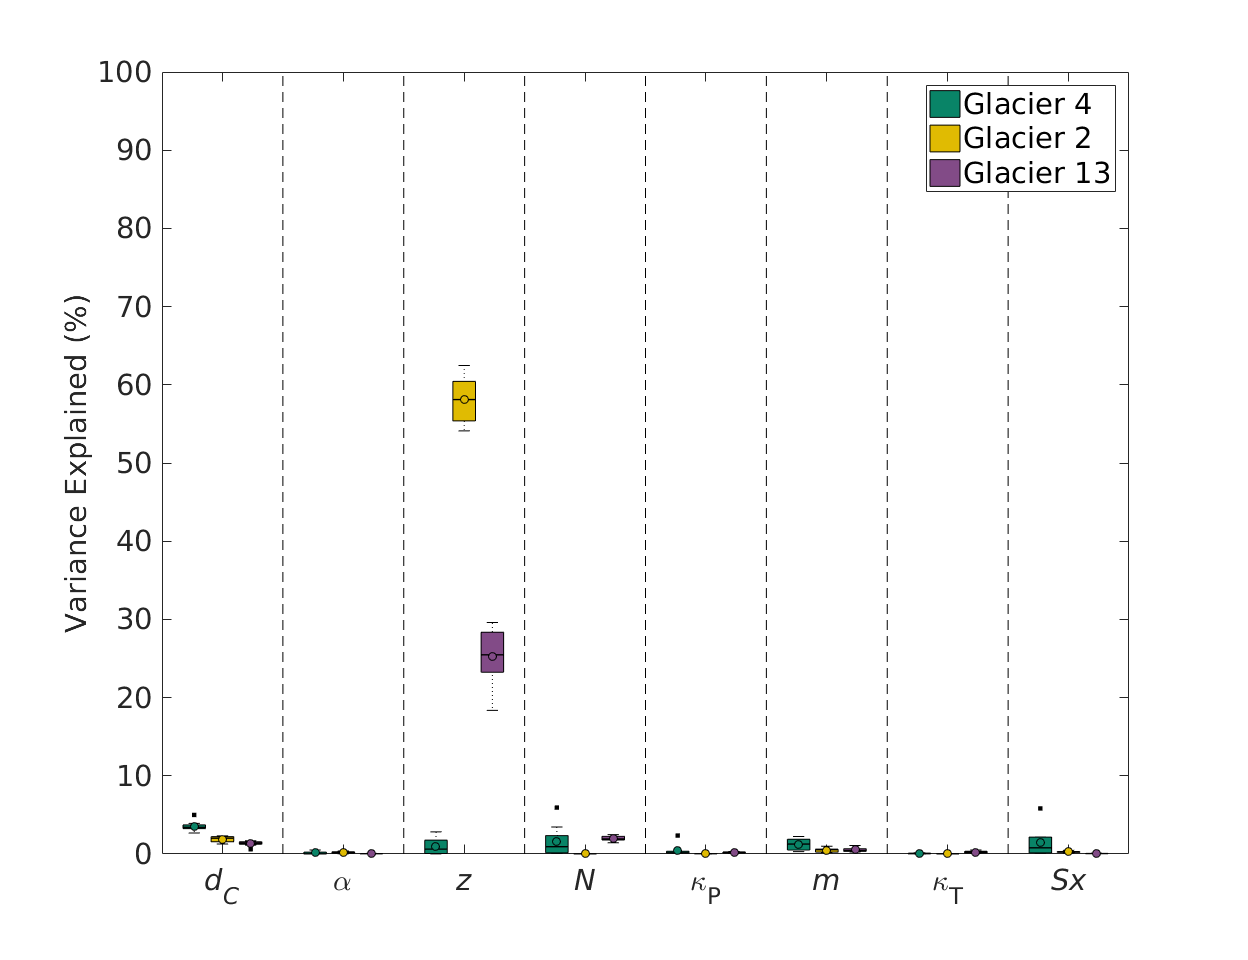
\includegraphics[width =1.1 \textwidth]{Coeffs_DensityOpts.png}\\
	\caption{Boxplot showing the range of percent variance explained by each topographic parameter for each option of estimating snow water equivalent (SWE). Topographic parameters include aspect ($\alpha$), elevation ($z$), northness ($N$), profile curvature ($\kappa_P$), slope ($m$), tangent curvature ($\kappa_T$), wind redistribution ($Sx$) and distance from centreline ($d_C$). Within each box, the mean is shown as a circle, the median as a horizontal line, the interquartile range (IQR) as a coloured box, two times the IQR as dashed lines beyond the box, and outliers as single points.}
	\label{fig:MLRPercentVar_densityOptions}
\end{figure} 

\begin{figure}[H]
	\makebox[\textwidth][c]{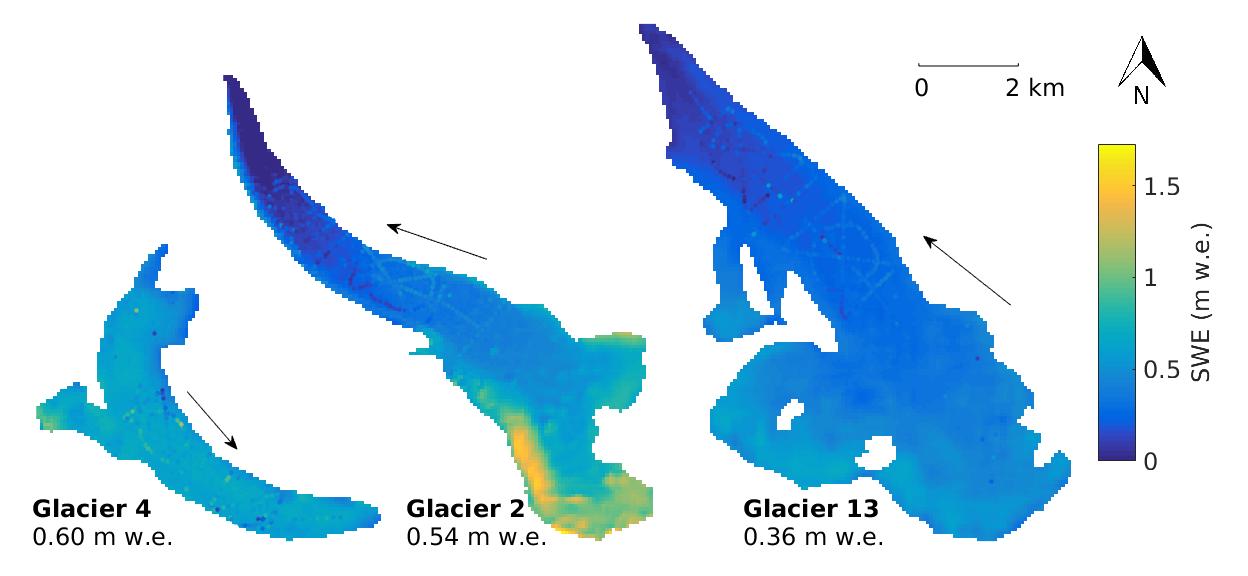
\includegraphics[width=\textwidth]{MLRmap_Modelled_Observed8.png}}%
	\caption{Modelled SWE using coefficients determined using MLR and density interpolated with inverse-distance weighting from snowpits (Option 7). Observed SWE values are overlain on the maps.}
	\label{fig:MLRmodelledSWE}
\end{figure}

\begin{figure}[H]
	\centering
	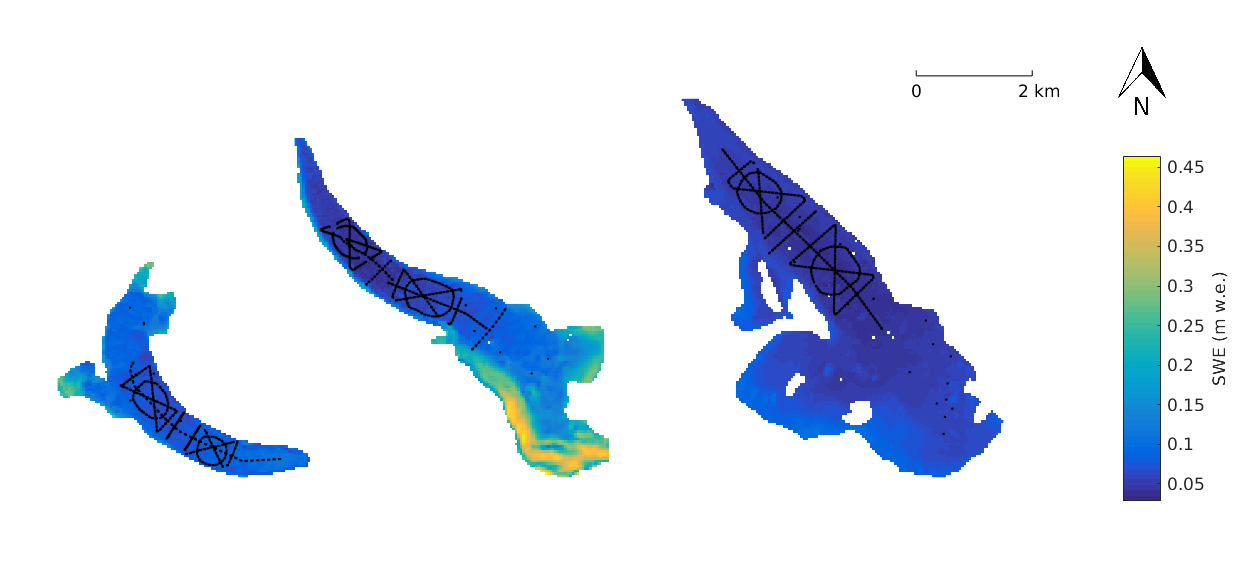
\includegraphics[width =\textwidth]{MLR_SWEdifferenceMap.png}\\
	\caption{Map of the difference between maximum and minimum SWE values for each DEM cell between all density options using MLR coefficients.}
	\label{fig:MLR_SWEdiffMap}
\end{figure}

 \begin{figure}[H]
	\centering
	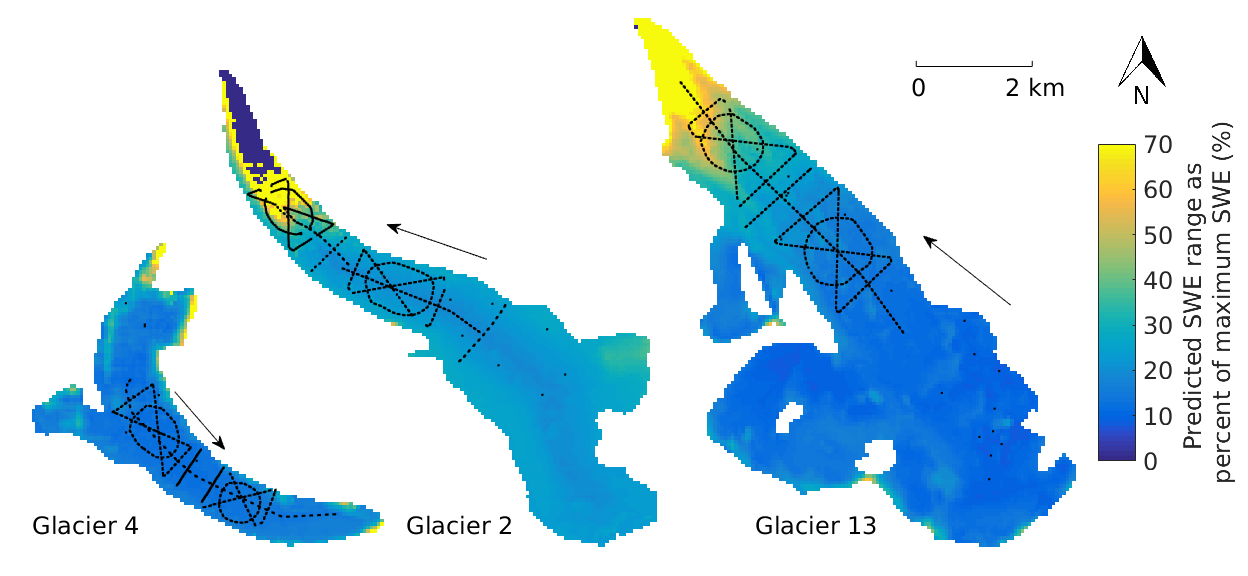
\includegraphics[width =\textwidth]{MLR_SWEdifferenceMap_percent.png}\\
	\caption{Map of the difference between maximum and minimum SWE values, expressed as a percent of the mean SWE, for each DEM cell between all density options using MLR coefficients. The colours have been scaled to highlight difference in the main part of the glaciers.}
	\label{fig:MLR_SWEdiffMapPercent}
\end{figure}
 


\begin{figure}
        \centering
        \begin{subfigure}[b]{0.475\textwidth}
            \centering
            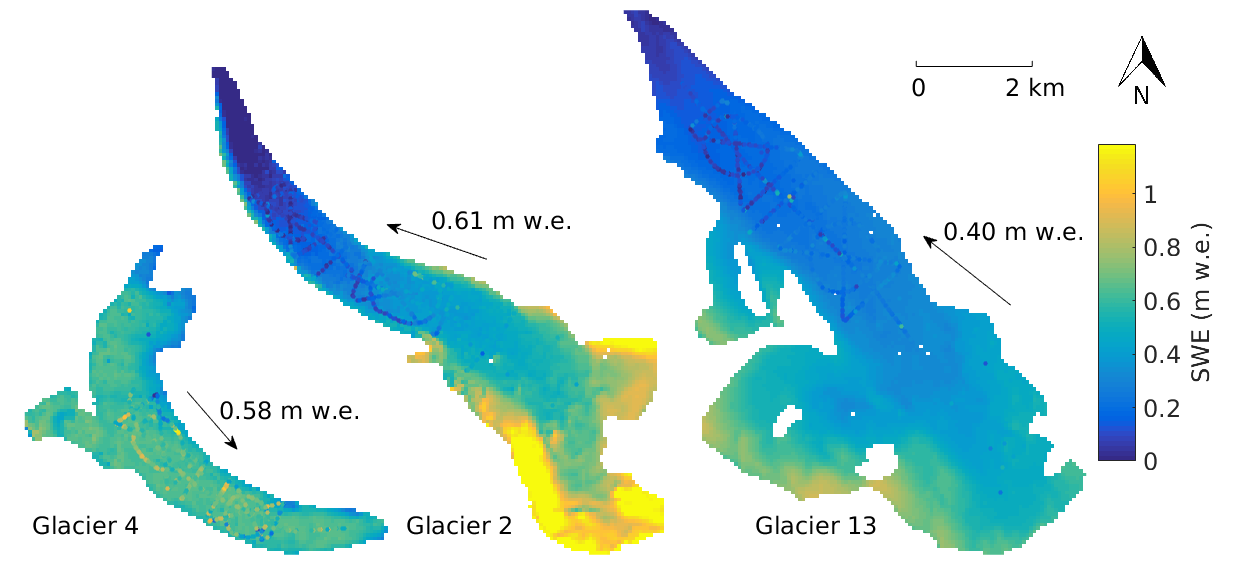
\includegraphics[width=\textwidth]{MLRmap_Modelled_Observed_Opt1.png}
            \caption[Option 1]%
            {{\small Option 1}}    
        \end{subfigure}
        \hfill
        \begin{subfigure}[b]{0.475\textwidth}  
            \centering 
            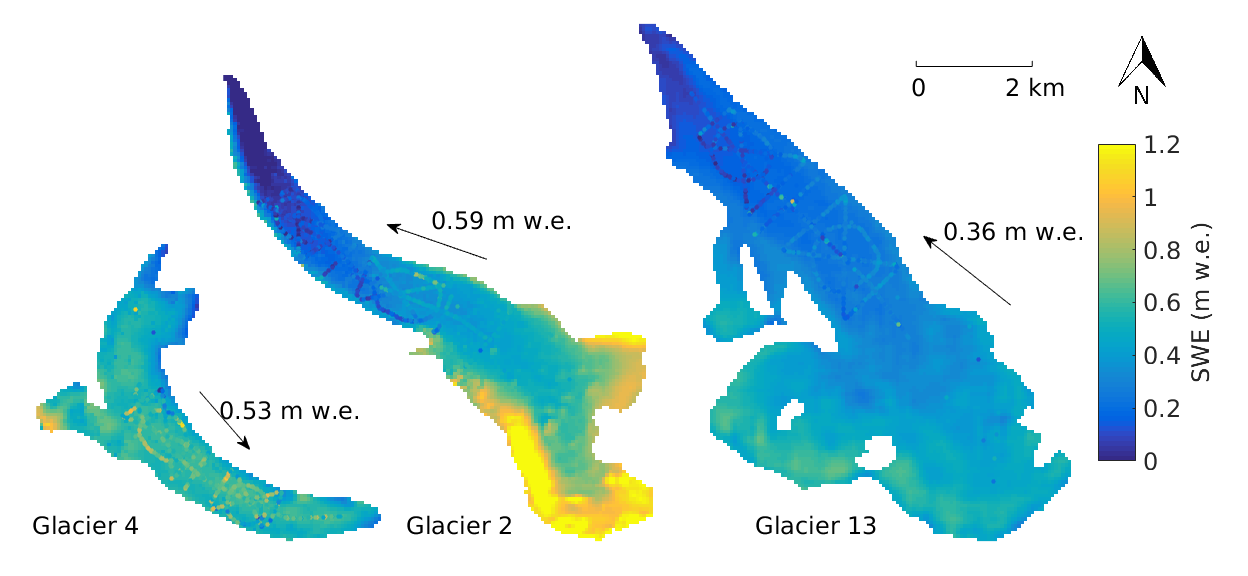
\includegraphics[width=\textwidth]{MLRmap_Modelled_Observed_Opt2.png}
            \caption[]%
            {{\small Option 2}}    
        \end{subfigure}
        \vskip\baselineskip
        \begin{subfigure}[b]{0.475\textwidth}   
            \centering 
            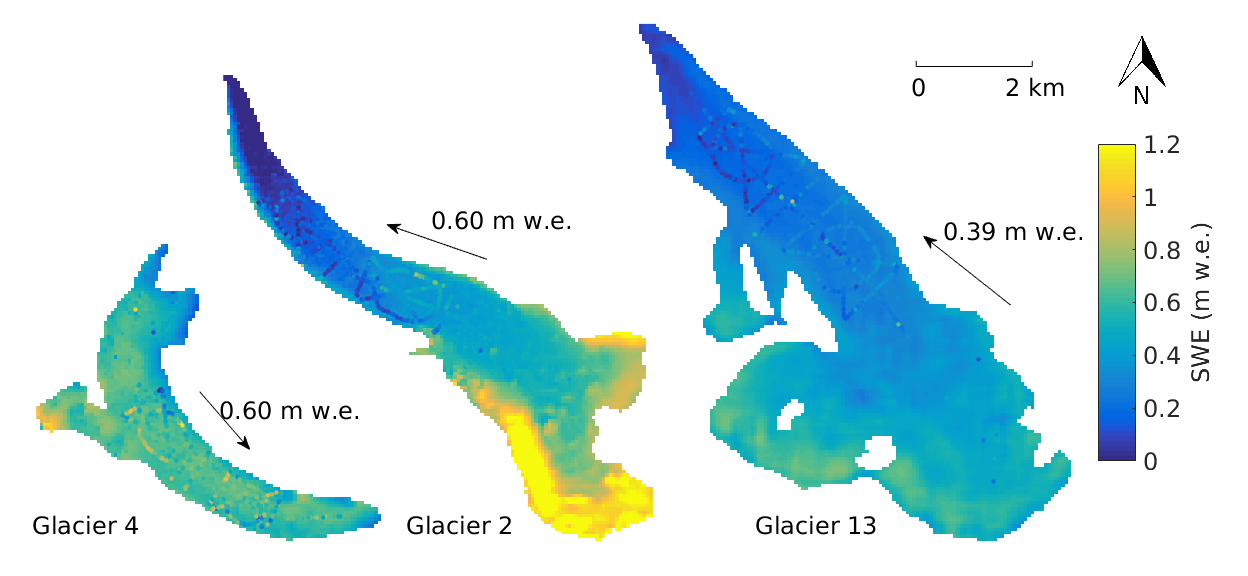
\includegraphics[width=\textwidth]{MLRmap_Modelled_Observed_Opt3.png}
            \caption[]%
            {{\small Option 3}}    
        \end{subfigure}
        \quad
        \begin{subfigure}[b]{0.475\textwidth}   
            \centering 
            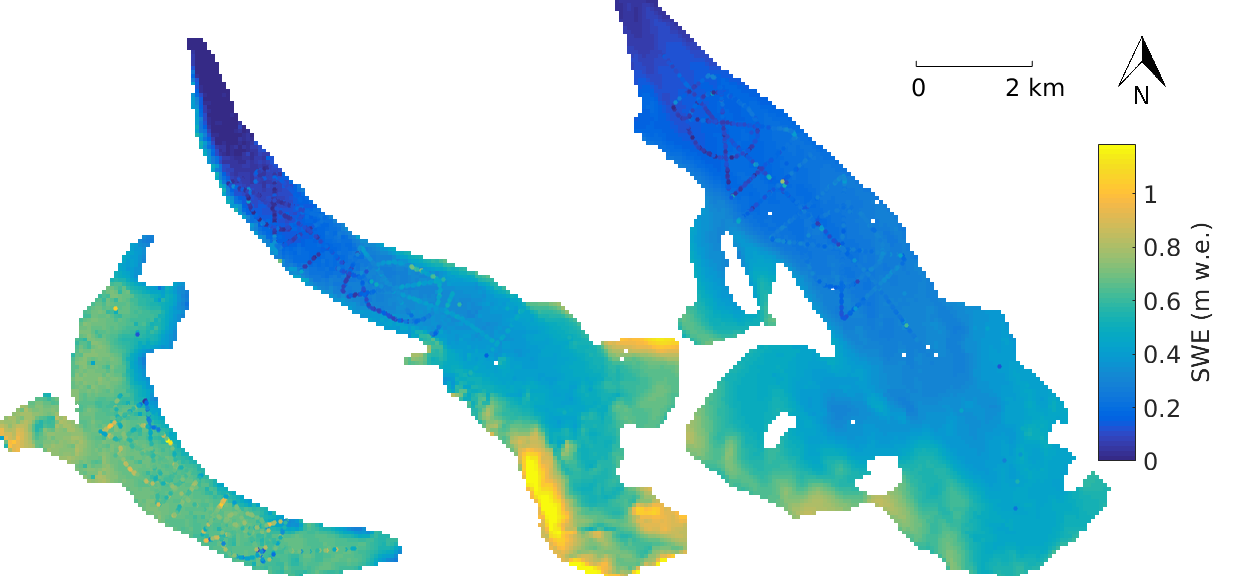
\includegraphics[width=\textwidth]{MLRmap_Modelled_Observed_Opt4.png}
            \caption[]%
            {{\small Option 4}}    
        \end{subfigure}
        
        \begin{subfigure}[b]{0.475\textwidth}
            \centering
            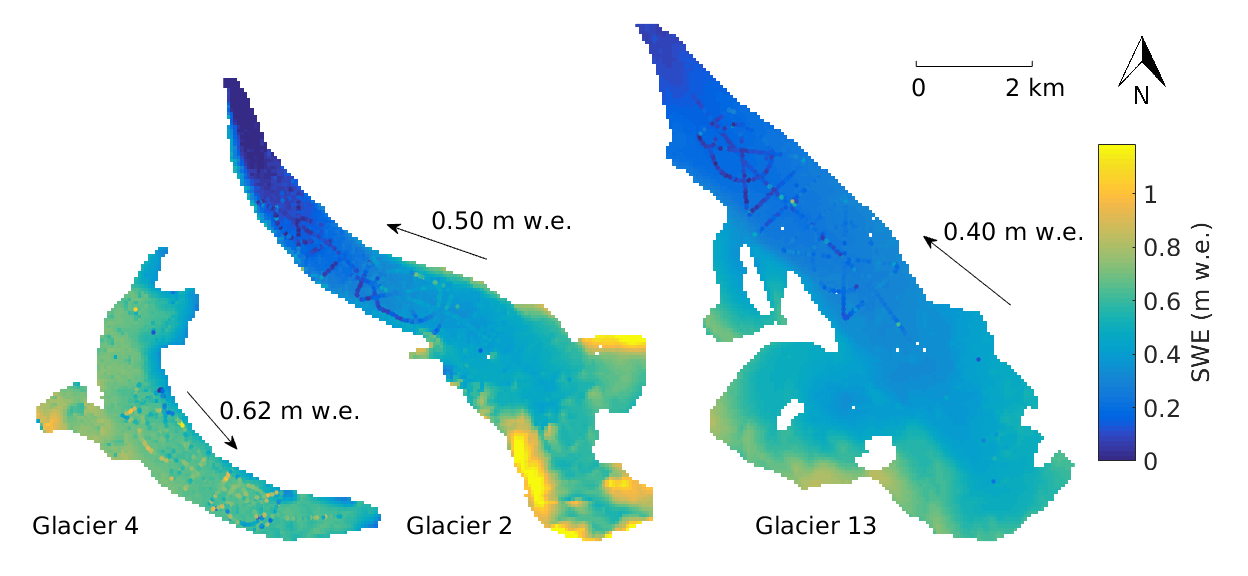
\includegraphics[width=\textwidth]{MLRmap_Modelled_Observed_Opt5.png}
            \caption[Option 5]%
            {{\small Option 5}}    
        \end{subfigure}
        \hfill
        \begin{subfigure}[b]{0.475\textwidth}  
            \centering 
            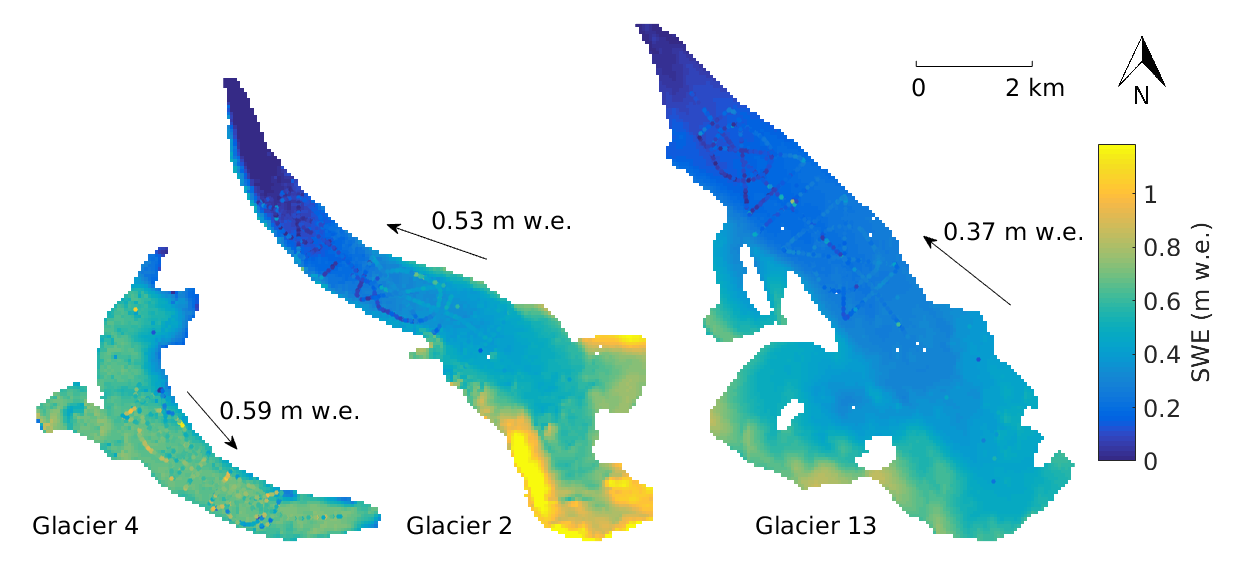
\includegraphics[width=\textwidth]{MLRmap_Modelled_Observed_Opt6.png}
            \caption[]%
            {{\small Option 6}}    
        \end{subfigure}
        \vskip\baselineskip
        \begin{subfigure}[b]{0.475\textwidth}   
            \centering 
            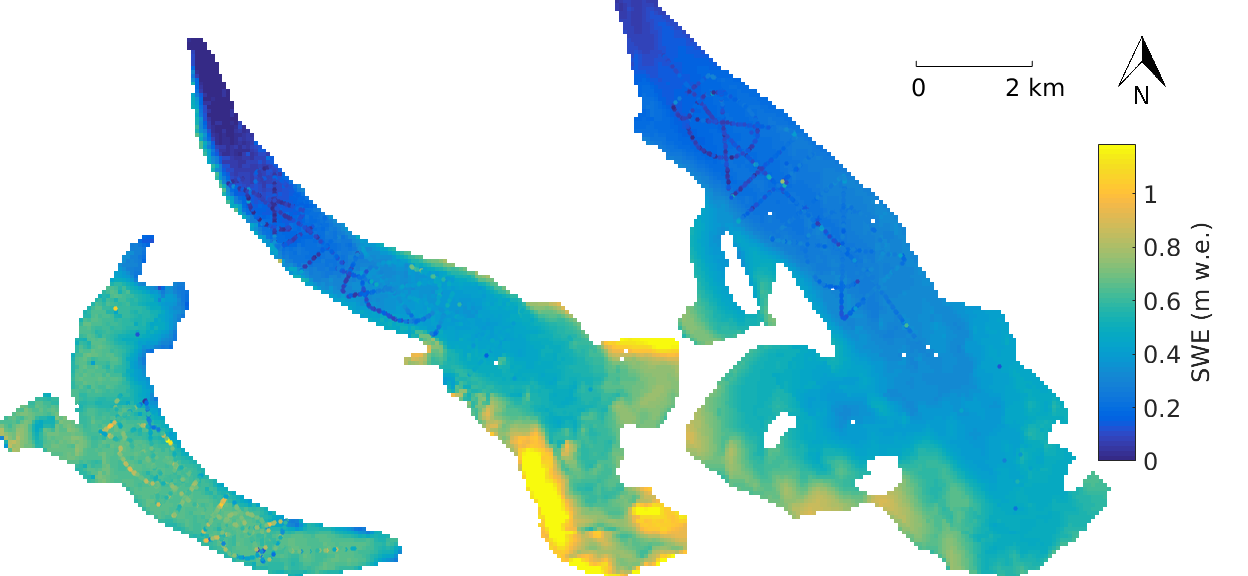
\includegraphics[width=\textwidth]{MLRmap_Modelled_Observed_Opt7.png}
            \caption[]%
            {{\small Option 7}}    
        \end{subfigure}
        \quad
        \begin{subfigure}[b]{0.475\textwidth}   
            \centering 
            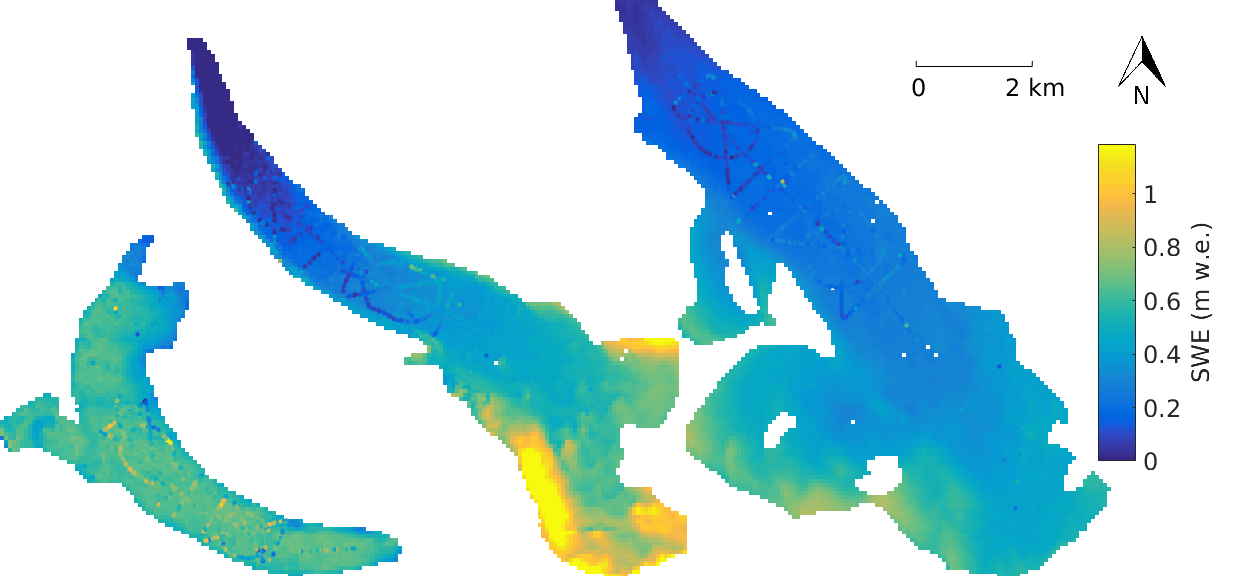
\includegraphics[width=\textwidth]{MLRmap_Modelled_Observed_Opt8.png}
            \caption[]%
            {{\small Option 8}}    
        \end{subfigure}
        
        \caption[Map of modelled SWE using the MLR coefficient values for all density options. Measured SWE is plotted as overlain filled circles.]
        {\small Map of modelled SWE using the MLR coefficient values for all density options. Measured SWE is plotted as overlain filled circles.} 
        \label{fig:allMLRmodelled}
    \end{figure}
    



%%%%%%%%%%%%%%%%%%%%%%%%%%%%%%%%%%%%%%%%%%%%%%%%%%
\subsection{Bayesian Model Averaging (BMA)}
\label{sec:BMS}

\subsubsection{Background}

\begin{wrapfigure}{L}{0.6\textwidth}
	\centering
	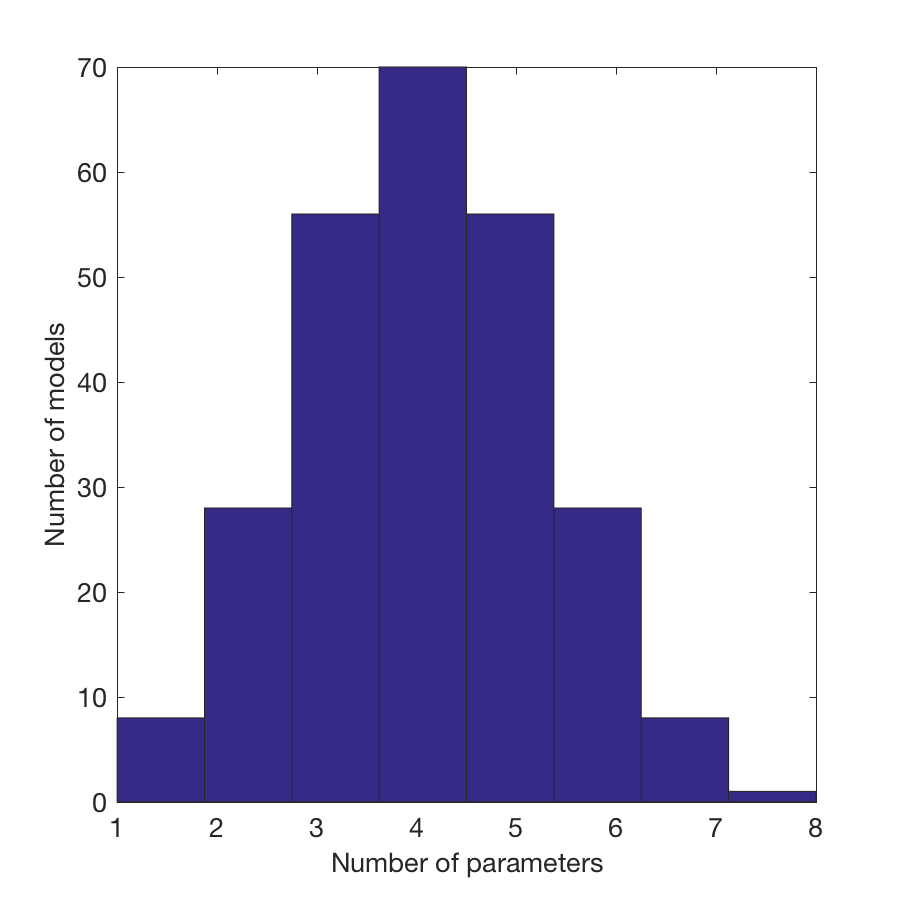
\includegraphics[width = 0.6\textwidth]{DistributionOfNumParams_topoRegress.png}\\
	\caption{Uniform model prior for eight topographic regressors used in BMA.}
	\label{fig:uni_model_prior}
\end{wrapfigure}

Bayesian model averaging (BMA) is a method of estimating all possible linear combinations of predictor variables, in this case topographic parameters, and then averaging over all models \citep{Raftery1997, Wasserman2000, Raftery2005}.  This method is based on Bayesian principals in which the probability of an outcome is determined based on an initial probably distribution that is determined by the researcher, as well as the data provided. Given that the predictive outcome has a probability distribution of $x$ given $y$, written as $P(x|y)$, we use Bayes' theorem to to write this as
\begin{equation}
P(x|y) = \frac{P(y|x)P(x)}{P(y)}.
\end{equation}•
$P(x|y)$ is often called the posterior model probability (PMP). The quantity $P(y|x)$ is the likelihood function, which determines unknown parameters from a known outcome (i.e. observed data). The term $P(x)$ is an observer determined prior probability distribution (typically just called a \textit{prior}) and it reflects the prior knowledge of the system \citep{Raftery1997}. Choosing an appropriate prior is one of the most challenge components of Bayesian probability theory \citep{Wasserman2000}. The $P(y)$ term can be obtained by integrating $P(y|x)P(x)$ over all $x$ and is thus a constant for all models that is typically discarded \citep{Wasserman2000}. 

Together then, the posterior model probability is a function of both the model prior, specified by the researcher, as well as the distribution of the observed data --- the PMP is the transformation of the prior as a result of considering collected data \citep{Wasserman2000}. This can be loosely expressed as
\begin{equation}
\textrm{posterior} \propto \textrm{prior} \times \textrm{likelihood}.
\end{equation}
If the prior is uninformative then the posterior will be strongly influenced by the data \citep{Wasserman2000}. An informative prior will result in a posterior that is a mix of the prior and the data. As the prior becomes more informative, the amount of data needed to transform the distribution increases. If there is a large amount of data then the prior will have little effect on the posterior. The final coefficients for the linear combination of predictor variables is often reported as posterior distribution means or values that maximize the log-likelihood. 

Within BMA, Bayes' theorem is used to find the posterior model probability and the PMP is used as a weight when averaging over all models \citep{Wasserman2000}. The model weighted posterior distribution for the coefficients $\beta$ of $k$ models after normalization is given by 
\begin{equation}
P(\beta| y,X) = \sum\limits_{i=1}^{2^k} P(M_i | X,y)P(\beta | M_i , y, X),
\end{equation}
where the responding variable is given by $y$ and the matrix of variables is given by $X$ \citep{Raftery1997}. Here, the model prior is $P(M_i | X,y)$ and the likelihood of the $\beta$ coefficient is $P(\beta | M_i , y, X)$.

There are a number of different priors to describe model size distribution that have been applied in BMA. A commonly used prior is the `uniform' prior, which assumes a normal model distribution with a total of $2^n$ models, where $n$ is the number of regressors \citep{Wasserman2000}.  This model prior states that the observer has no knowledge of the system and all models are equally likely. The uniform prior has a prior model probability of the form $P(M_i)=2^{-n}$ (Figure \ref{fig:uni_model_prior}), which is symmetric about the mean $n/2$ \citep{Zeugner2015}. This prior inherently favours models of an intermediate size. 

Other types of priors include those that are skewed to favour smaller models, ones with equal probability for all model sizes, and ones with varying probability for individual regressors. In this project, a uniform prior was chosen for two reasons. First, there was no knowledge of the model distribution so we aim to minimize the observer influence on the final distribution. Second, the MLR estimation (Section \ref{sec:MLR}) assumes a uniform distribution so chosing a uniform distribution for BMA allows for consistency between methods. Using a uniform distribution is commonly done in BMA \citep{Wasserman2000}.

With a small number of regressors, the posterior of all possible models can be determined. However, with a large set of regressors, this computation becomes increasingly expensive. To reduce computation time for a large set of regressors, BMA can use Markov chain Monte Carlo (MCMC) model composition to directly approximate the posterior distribution \citep{Wasserman2000}. In our study, there are eight regressors so $2^8 = 256$ models. It is possible to visit all models and to obtain an exact solution so an MCMC model composition was not employed. 

BMA allows for the calculation of a metric called the posterior inclusion probability (PIP), which is used to evaluate the importance of a regressor in explaining the observed data. PIP is the sum of all posterior model probabilities (PMP) where the variable was included in the model \citep{Zeugner2015}. A higher PIP indicates that the regressor is more important in the regression.  

\subsubsection{Methods}

The BMA process was implemented in R, using the Bayesian model statistics (BMS) package developed by \cite{Zeugner2015}. The function \texttt{BMS\_R()} computes the posterior distribution mean value of all $\beta$ coefficients for topographic parameters as well as the percent variance explained by each parameter using the following steps:
\begin{enumerate}
\item A portion of the data ($2/3$ as suggested by \cite{Kohavi1995}) is randomly chosen as the calibration set and saved as a .mat file. 
\item The Bayesian model statistics (BMS) package developed by \cite{Zeugner2015} is run in R (called through an operating system command in Matlab)
	\begin{enumerate}
		\item The R script imports the .mat file with SWE and topographic parameter values. It then creates a data 				frame with the SWE values as the first column and the topographic parameters as the remaining 					columns. 
		\item The BMS package is used to complete BMA for the imported values. A uniform model prior was chosen. 				The mean coefficient value, coefficient standard deviation, PIP, and the posterior probability of a positive 			coefficient (how probable it is for the sign of the coefficient to be positive) were computed.
		\item The coefficients are saved as a .mat file.
	\end{enumerate}
\item Regressor coefficient values calculated in R are loaded into Matlab and a data table is created with the coefficients.
\item The remaining portion of the data ($1/3$) are then used to calculate a modelled value of SWE at those locations. These are compared to the observed SWE values and a RMSE value is determined.
\item The above steps are completed 1000 times and the coefficients associated with the lowest RMSE are chosen.
\item Percent variance explained by each parameter is then calculated in the same way as for the MLR (see Section 			\ref{sec:MLRMethods}). 
\item The final table of values includes the coefficients and percent variance explained for all topographic parameters associated with the lowest RMSE. It also includes the intercept and the actual RMSE value. This table is returned from the function.
\item The residuals of the best BMA fit are also calculated and can be return from the function.  
\end{enumerate}

\subsubsection{Results and Discussion}

The coefficients determined using BMA for density Option 7 can be seen in Table \ref{tab:BMScoeff} and can be used to examine the relative importance of topographic parameters in the regression. These coefficients were found for standardized values of topographic parameters so their magnitude is indicative of their importance in predicting SWE. Table \ref{tab:BMScoeffFull} shows coefficient values for all density options. The range of percent variance explained by each variable (from all density options) can be seen in Figure \ref{fig:BMSPercentVar_densityOptions}. The fit between modelled SWE and observed SWE for each glacier for density option 7 can be seen in Figure \ref{fig:BMSfit_opt8} and the fit for all density options in Figure \ref{fig:BMSfit_allLines}. The distribution of residuals in then plotted in Figure \ref{fig:BMSresiduals_all}. A map of the predicted values of SWE over the entire glacier using density option 7 can be seen in Figure \ref{fig:BMSmodelledSWE} with basic summary statistics found in Table \ref{tab:BMSsweMinMax}. Modelled SWE using all density options is shown in Figure \ref{fig:allBMSmodelled}. A map of the difference between maximum and minimum modelled SWE values is shown in Figure \ref{fig:BMS_SWEdiffMap}.

\begin{wraptable}{R}{10cm}
\centering
\caption{BMS coefficients for topographic regression between measured SWE and standardized topographic parameters that include distance from centreline ($d_C$), elevation ($z$), aspect ($\alpha$),slope ($m$), northness ($N$), profile curvature ($\kappa_P$), tangent curvature ($\kappa_T$), and wind redistribution ($Sx$). SInce parameters are standardizes, the magnitude of the coefficients is representative of their importance in predicting SWE. The root-mean-squared error (RMSE) between modelled SWE using those coefficients and observed SWE is also given.}
\label{tab:BMScoeff}
\begin{tabular}{cccc}
 & \textbf{Glacier 4} & \textbf{Glacier 2} & \textbf{Glacier 13} \\ \hline
d$_C$ 			& -0.004 					& 0.020 	& 0.007 \\
$z$ 				&  0.013 					& 0.107 	& 0.047 \\
$\alpha$ 		& 0.002 					& -0.008 	& -0.010 \\
$m$ 			& -0.020 					& 0.011 	&  \textless-0.001 \\
$N$ 				&   \textless-0.001 	& 0.004 	& 0.001 \\
$\kappa_P$ 	&  \textless0.001 	& 0.003 	&\textless -0.001 \\
$\kappa_T$ 	& \textless0.001 		& 0.002 	& -0.003 \\
$Sx$ 			& -0.027 					& 0.040 	& 0.007 \\
Intercept 		& 0.619 					& 0.268 	& 0.238 \\ \hline
RMSE 			& 0.136 					& 0.098	& 0.086 
\end{tabular}
\end{wraptable}

For Glacier 4, the largest coefficients are wind redistribution ($Sx$), slope, and elevation, which are an order of magnitude larger than the remaining coefficients. The $Sx$ and slope coefficients are negative, which indicates less snow in `sheltered' areas and less on steeper slopes. The elevation coefficient is positive, indicating that there is more snow at higher elevation. These coefficients account for the largest percentage of variance explained, although this percentage is small ($\sim$7\%, $\sim$1\% and $\sim$1\%, respectively). Overall, the modelled winter balance for Glacier 4 is very poorly explained by the topographic parameters, which results in no correlation between modelled and observed SWE (R$^2_{avg}=0.05$) and a comparatively high RMSE value. The modelled values of SWE are largely determined by the intercept value. The map of predicted SWE for the entire glacier shows a relatively uniform SWE distribution over Glacier 4, likely due to the large influence of the intercept on the regression. The variation of SWE across the width of the glacier is not captured by the regression. Modelled values on glacier right are less than observed and on glacier left the modelled values are greater than observed. This regression indicates that the wind effects play a significant role in snow distribution but since the valley in which the glacier sits is steep walled and curved, perhaps having a single cardinal direction for wind is inappropriate. Examining $Sx$ values that assume wind moving up or down glacier and changing direction to follow the valley could allow the $Sx$ parameter to explain more of the variance. 
\begin{wraptable}{l}{8.5cm}
\centering
\caption{Basic summary statistics of modelled SWE using coefficients found using BMA. Values are for coefficients determined using SWE with inverse distance weighted snowpit densities. }
\label{tab:BMSsweMinMax}
\begin{tabular}{lccc}
\multicolumn{1}{l}{} & \multicolumn{3}{c}{\textbf{Modelled SWE (m w.e.)}} \\
                     & Mean          & Minimum          & Maximum         \\ \hline
Glacier 4            & 0.58          & 0.26             & 0.75            \\
Glacier 2            & 0.57          & -0.25            & 1.76            \\
Glacier 13           & 0.39          & 0.02             & 0.85           
\end{tabular}
\end{wraptable} 
For Glacier 2, the largest coefficient (by an order of magnitude) is elevation. This coefficient is positive, which means that SWE will increase with elevation. Elevation explains the largest amount of variance ($\sim$45\%). $Sx$, distance from centreline, and slope are also significant coefficients in BMA, explaining $\sim$6\%, $\sim$1\% and $\sim$1\% of the variance, respectively.  Overall, the modelled winter balance is a good estimation of observed SWE (R$^2_{avg}=0.62$) although it tends to underestimate the amount of accumulation. The map of modelled SWE shows the strong dependence on elevation since the values closely resemble the elevation map (Figure \ref{map:elev}). The range of predicted SWE is largest for Glacier 2 and it also has the highest SWE and the lowest SWE values. Although negative values are inconsistent with with accumulation, they do reflect the lack of snow cover over the lower portion of the terminus. 

For Glacier 13, the largest coefficient is elevation with aspect also of the same order of magnitude. The elevation coefficient is positive, which means that cells at higher elevation had higher amounts of SWE. The aspect coefficient was negative, which indicates that larger values of aspect correspond to less snow. Elevation explains the majority of the variance (24\%), while aspect explains far less ($<$1\%).  Overall, the MLR modelled winter balance is poorly related to observed SWE (R$^2_{avg}=0.34$) and tends to underestimate the amount of accumulation. The map of modelled SWE displays an increase with elevation, although it is not strong considering the large range of elevation on this glacier.

Qualitatively, there is little variation in the fit between modelled and observed winter balance between the various density options for all glaciers and the residuals display a similar distribution between the density options.The percent variance explained by each parameter also varies little between different density options. 

The effect of density values on the percent variance explained by each topographic parameters from BMA is shown in Figure \ref{fig:BMSPercentVar_densityOptions}. The range of percent variance explained by elevation is large for both Glacier 2 and 13 but it does not affect the importance of elevation relative to the other parameters. For these two BMA coefficients, the choice of density interpolation has a large effect on the ability of the model to explain variance in SWE. Using elevation regressed Federal Sampler derived density resulted in the highest percent variance explained (59\%). Since the Federal Sampler derived densities are correlated with snow depth, which is correlated with elevation, it is likely that these density values amplify the elevation component of the regression. The range of percent variance explained for all other parameters is small so the BMA coefficients for these parameters are insensitive to the choice of density interpolation. The values for ``northness'' and both curvatures are essentially zero and have negligible ranges. 

\begin{figure}[H]
	\makebox[\textwidth][c]{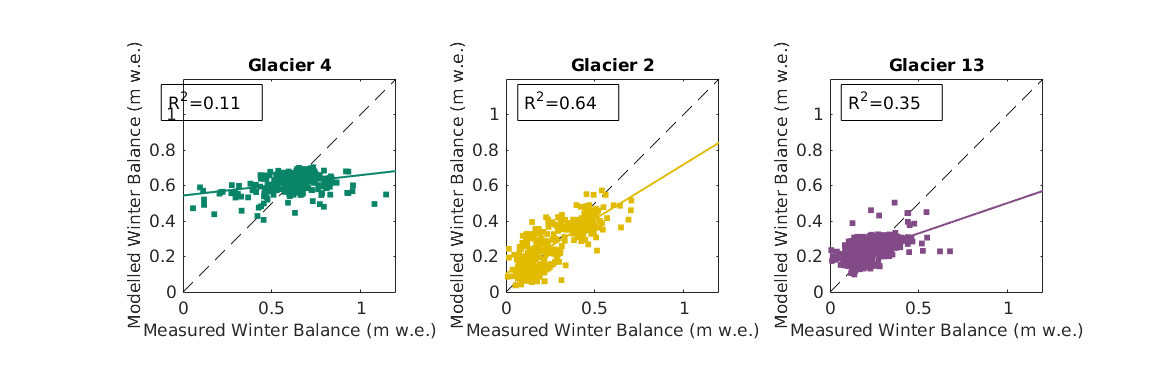
\includegraphics[width=1.2\textwidth]{BMSfit_opt8.png}}%
	\caption{Comparison of predicted (BMA) and observed (original) snow water equivalent (SWE) for three study glaciers. The SWE values were calculated inverse distance weighted snowpit densities (Option 7).}
	\label{fig:BMSfit_opt8}
\end{figure}

\begin{figure}[H]
	\makebox[\textwidth][c]{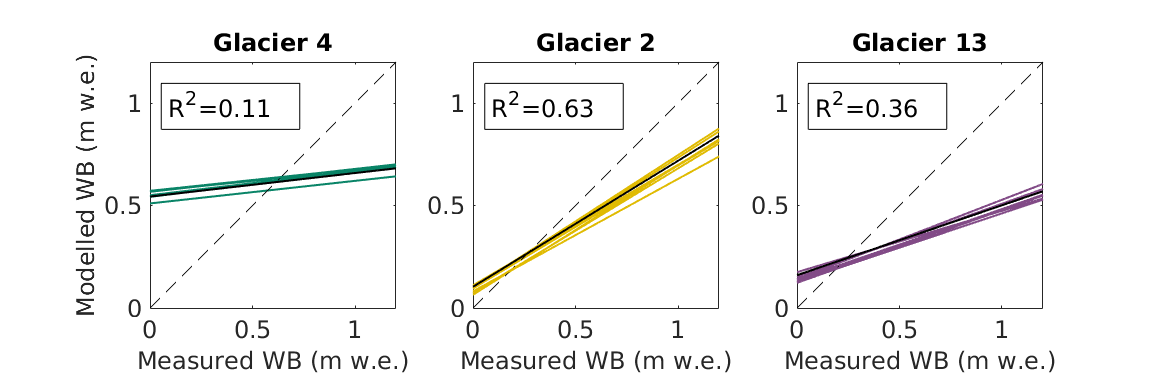
\includegraphics[width=1.2\textwidth]{BMSfit_allLines.png}}%
	\caption{Plot of all linear fits between modelled (BMA) and observed SWE using eight options for calculating density. Mean R$^2$ value is shown for each sub-plot and a reference 1:1 line is also provided. See Figure \ref{fig:BMSfit_opt8} for a plot of the data. }
	\label{fig:BMSfit_allLines}
\end{figure}

\begin{figure}[H]
	\makebox[\textwidth][c]{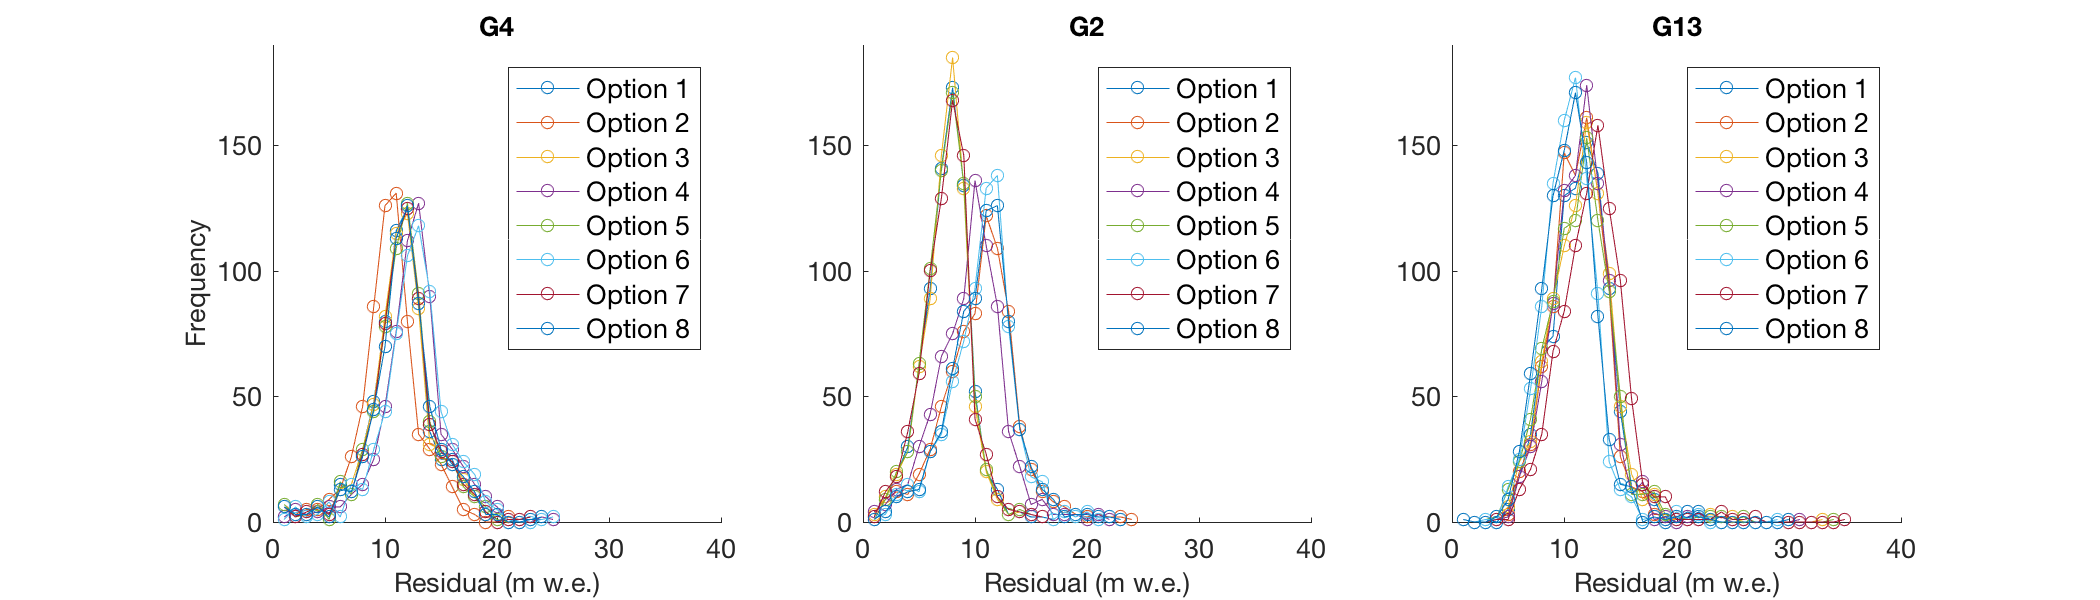
\includegraphics[width=1.2\textwidth]{BMSresiduals_all.png}}%
	\caption{Residuals of SWE predicted using BMA for all options of estimating density.}
	\label{fig:BMSresiduals_all}
\end{figure}

\begin{figure}[H]
	\makebox[\textwidth][c]{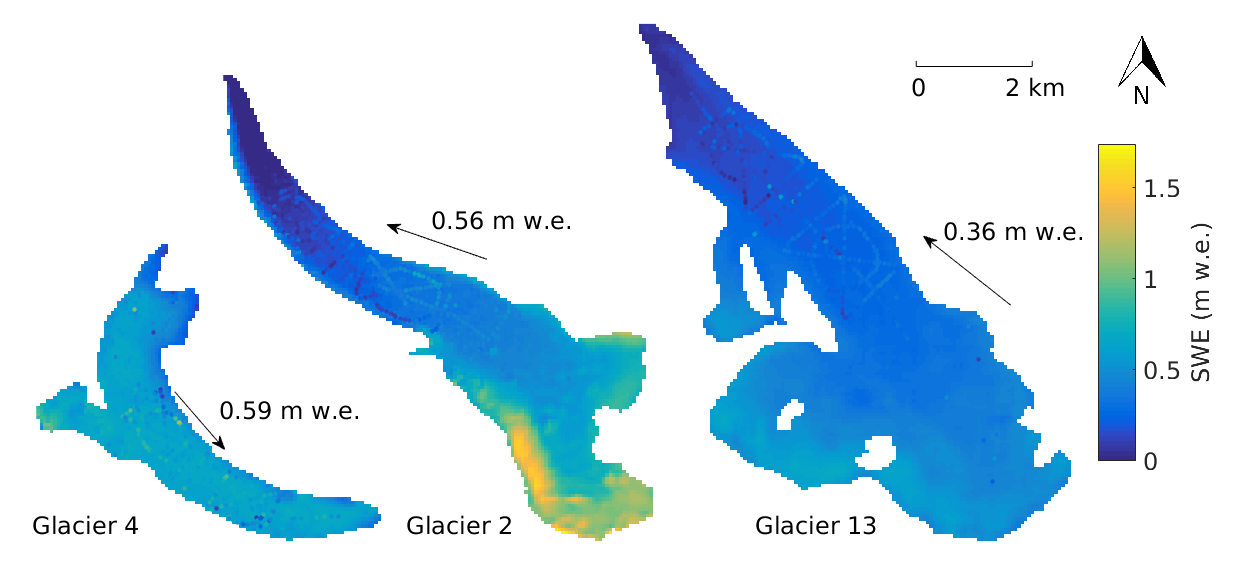
\includegraphics[width=\textwidth]{BMSmap_Modelled_Observed8.png}}%
	\caption{Modelled SWE using coefficients determined using BMA and density interpolated with inverse-distance weighting from snowpits (option 7). Observed SWE values are overlain on the maps.}
	\label{fig:BMSmodelledSWE}
\end{figure}
 
\begin{figure}[H]
	\centering
	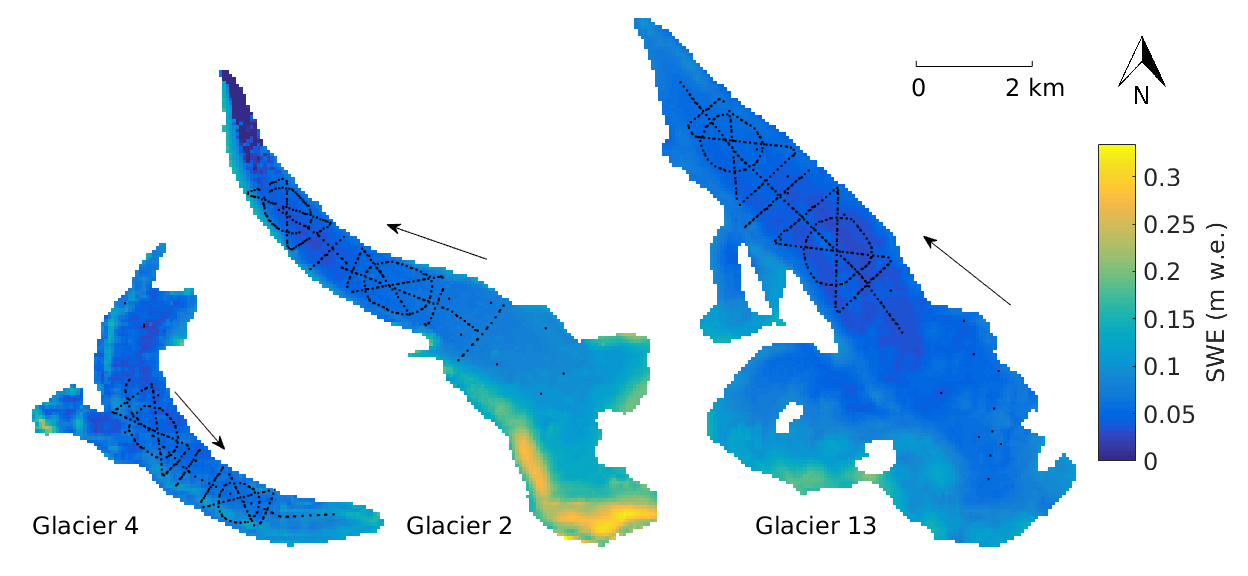
\includegraphics[width =\textwidth]{BMS_SWEdifferenceMap.png}\\
	\caption{Map of the difference between maximum and minimum SWE values for each DEM cell between all density options using BMA coefficients.}
	\label{fig:BMS_SWEdiffMap}
\end{figure} 
 
 \begin{figure}[H]
	\centering
	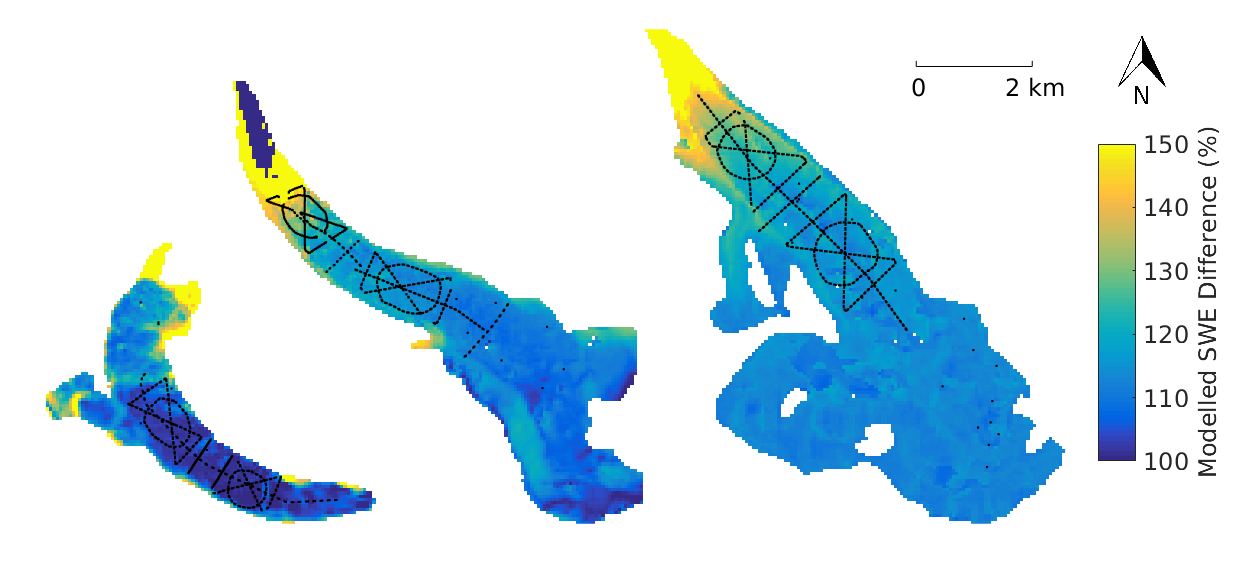
\includegraphics[width =\textwidth]{BMS_SWEdifferenceMap_percent.png}\\
	\caption{Map of the difference between maximum and minimum SWE values, expressed as a percent of the mean SWE, for each DEM cell between all density options using BMA coefficients. The colours have been scaled to highlight difference in the main part of the glaciers.}
	\label{fig:BMS_SWEdiffMap}
\end{figure} 

\begin{figure}[H]
	\centering
	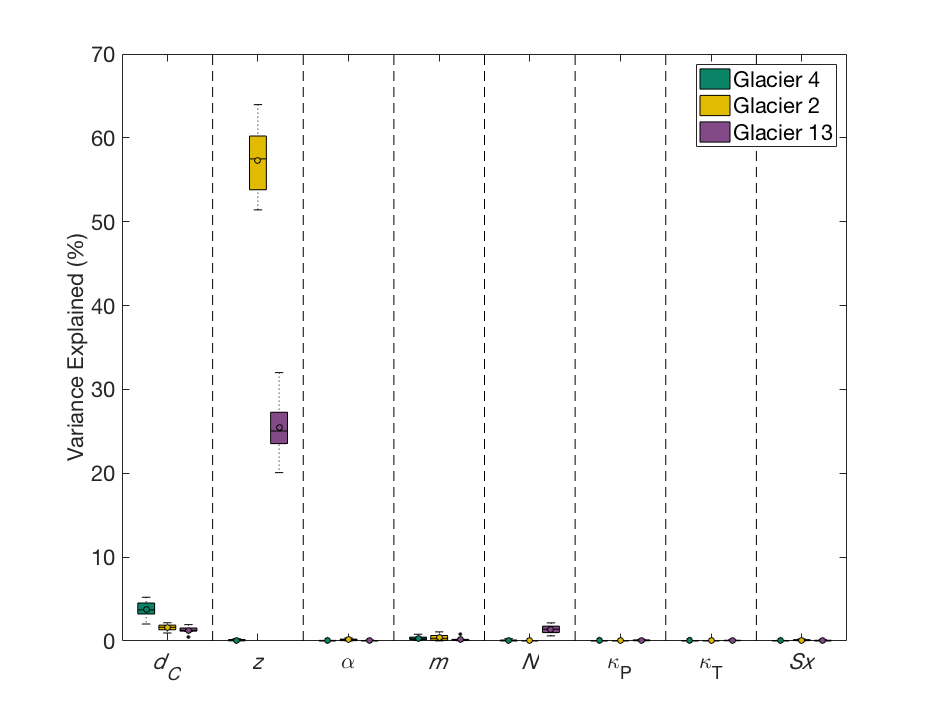
\includegraphics[width = 1.1 \textwidth]{BMSCoeffs_DensityOpts.png}\\
	\caption{Boxplot showing the range of percent variance explained by each topographic parameter as calculated using BMA for each option of estimating snow water equivalent (SWE). \params \boxplot}
	\label{fig:BMSPercentVar_densityOptions}
\end{figure} 

\begin{figure*}
        \centering
        \begin{subfigure}[b]{0.475\textwidth}
            \centering
            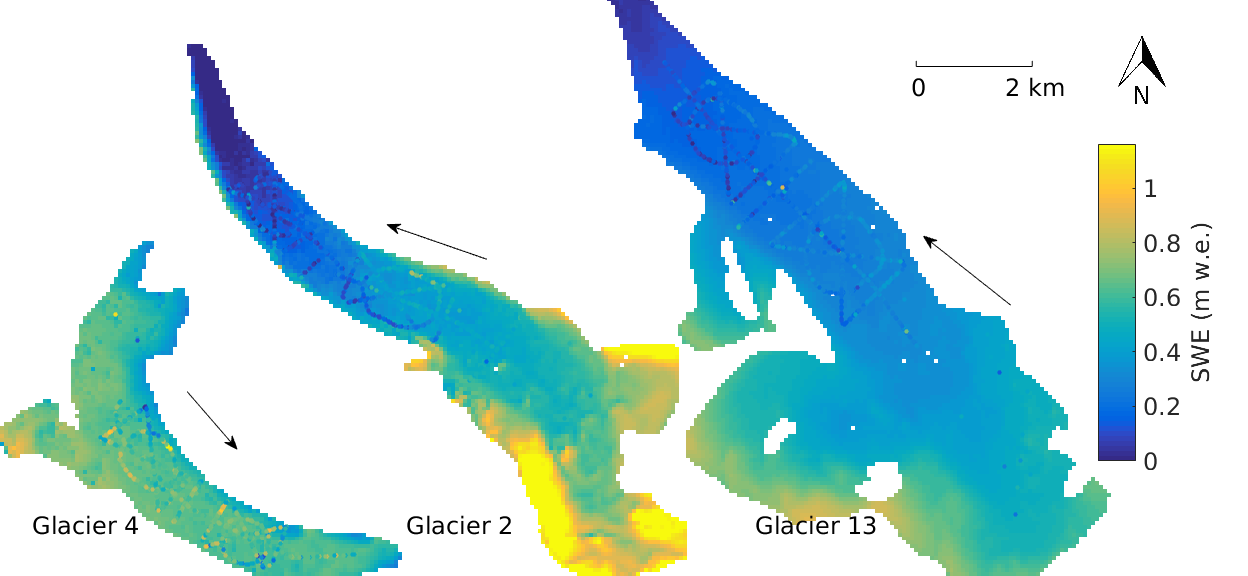
\includegraphics[width=\textwidth]{BMSmap_Modelled_Observed_Opt1.png}
            \caption[Option 1]%
            {{\small Option 1}}    
        \end{subfigure}
        \hfill
        \begin{subfigure}[b]{0.475\textwidth}  
            \centering 
            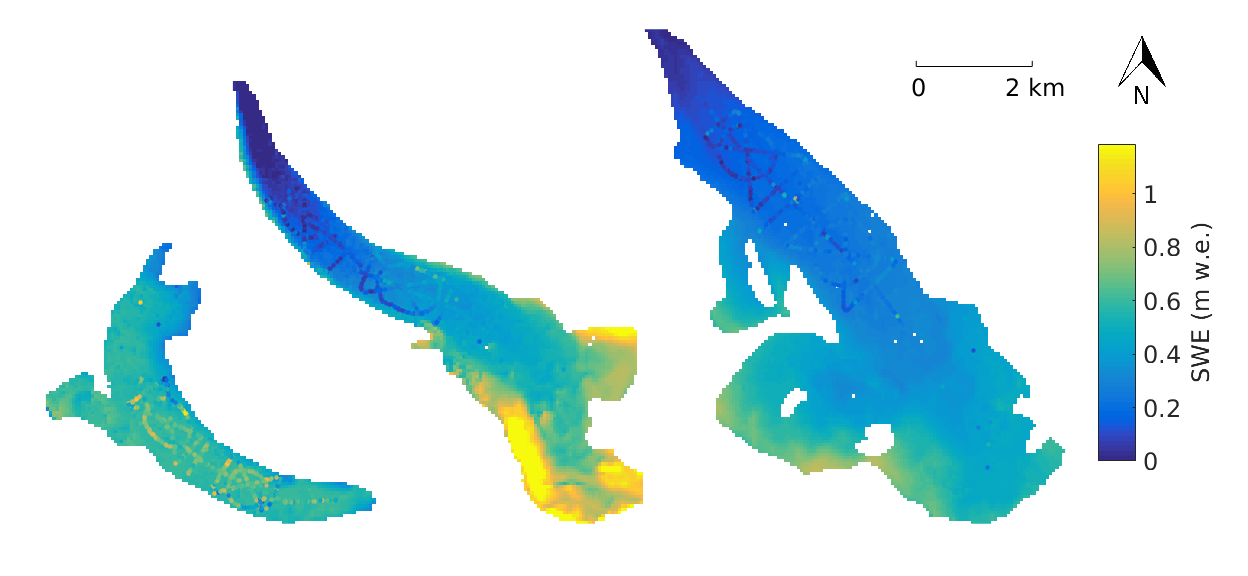
\includegraphics[width=\textwidth]{BMSmap_Modelled_Observed_Opt2.png}
            \caption[]%
            {{\small Option 2}}    
        \end{subfigure}
        \vskip\baselineskip
        \begin{subfigure}[b]{0.475\textwidth}   
            \centering 
            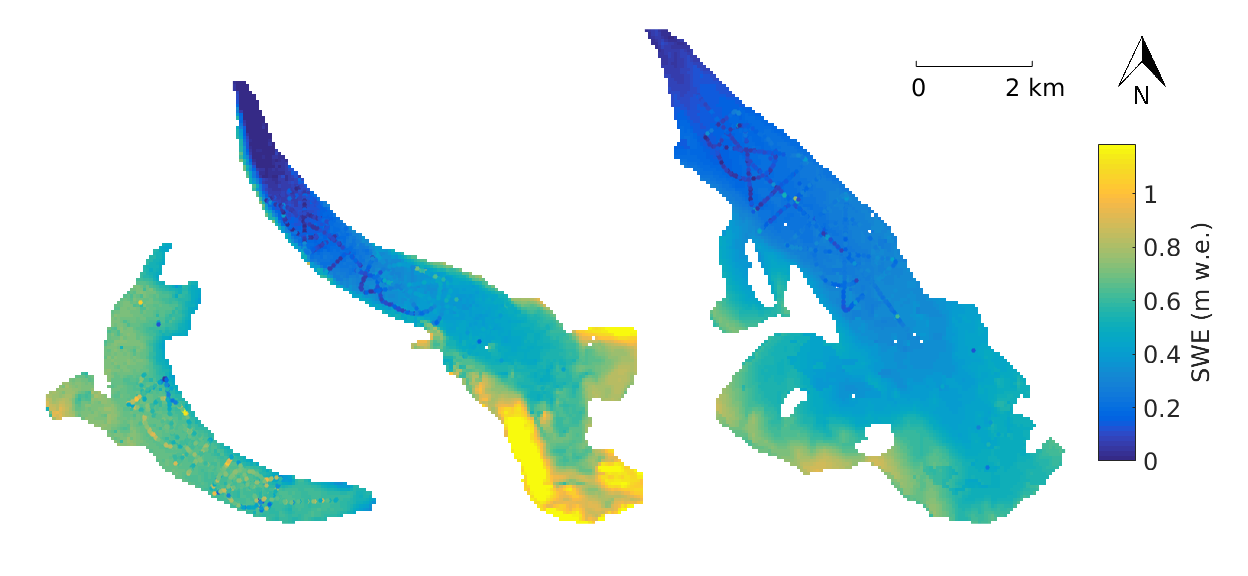
\includegraphics[width=\textwidth]{BMSmap_Modelled_Observed_Opt3.png}
            \caption[]%
            {{\small Option 3}}    
        \end{subfigure}
        \quad
        \begin{subfigure}[b]{0.475\textwidth}   
            \centering 
            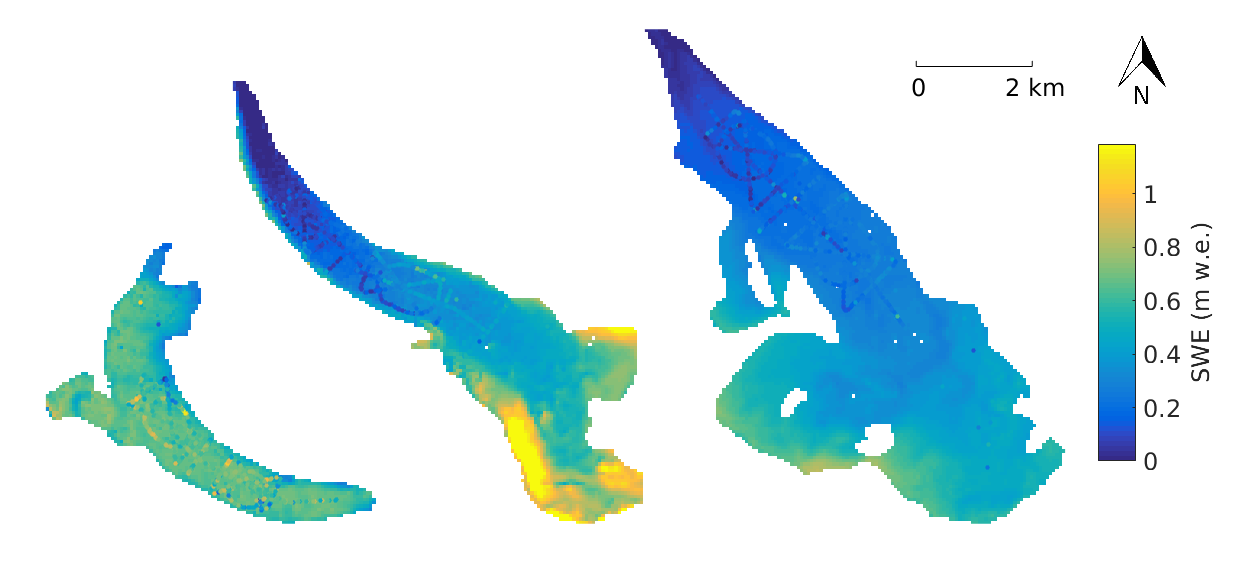
\includegraphics[width=\textwidth]{BMSmap_Modelled_Observed_Opt4.png}
            \caption[]%
            {{\small Option 4}}    
        \end{subfigure}
        
        \begin{subfigure}[b]{0.475\textwidth}
            \centering
            \includegraphics[width=\textwidth]{BMSmap_Modelled_Observed_Opt5.png}
            \caption[Option 5]%
            {{\small Option 5}}    
        \end{subfigure}
        \hfill
        \begin{subfigure}[b]{0.475\textwidth}  
            \centering 
            \includegraphics[width=\textwidth]{BMSmap_Modelled_Observed_Opt6.png}
            \caption[]%
            {{\small Option 6}}    
        \end{subfigure}
        \vskip\baselineskip
        \begin{subfigure}[b]{0.475\textwidth}   
            \centering 
            \includegraphics[width=\textwidth]{BMSmap_Modelled_Observed_Opt7.png}
            \caption[]%
            {{\small Option 7}}    
        \end{subfigure}
        \quad
        \begin{subfigure}[b]{0.475\textwidth}   
            \centering 
            \includegraphics[width=\textwidth]{BMSmap_Modelled_Observed_Opt8.png}
            \caption[]%
            {{\small Option 8}}    
        \end{subfigure}
              
        \caption[Map of modelled SWE using the BMS coefficient values for all density options. Measured SWE is plotted as overlain filled circles.]
        {\small Map of modelled SWE using the BMS coefficient values for all density options. Measured SWE is plotted as overlain filled circles.} 
        \label{fig:allBMSmodelled}
    \end{figure*}
  
\begin{landscape}
\begin{table}
\centering
\caption{Topographic regression coefficients determined using BMA. See Table \ref{tab:densityOptions} for description of density options.}
\label{tab:BMScoeffFull}
\begin{tabular}{cccccccccc}
 & \textbf{\begin{tabular}[c]{@{}c@{}}Topographic \\ Parameter\end{tabular}} & \textbf{Option 1} & \textbf{Option 2} & \textbf{Option 3} & \textbf{Option 4} & \textbf{Option 5} & \textbf{Option 6} & \textbf{Option 7} & \textbf{Option 8} \\ \hline
 
 & $d_C$ & -0.004 & -0.002 & -0.002 & 0.000 & -0.007 & -0.004 & -0.004 & 0.000 \\
 
 & $z$ & 0.021 & 0.005 & 0.028 & 0.007 & 0.028 & 0.000 & 0.012 & 0.001 \\
 
 & $\alpha$ & 0.003 & 0.003 & 0.001 & 0.001 & 0.000 & 0.001 & 0.002 & 0.001 \\
 
 & $m$ & -0.006 & -0.010 & -0.008 & -0.022 & -0.016 & -0.005 & -0.020 & -0.029 \\
 
 & $N$ & -0.006 & 0.000 & 0.000 & -0.006 & -0.003 & -0.001 & 0.001 & 0.000 \\
 
 & $\kappa_P$ & 0.000 & -0.001 & 0.000 & -0.002 & -0.011 & 0.000 & 0.000 & -0.003 \\
 
 & $\kappa_T$ & 0.000 & 0.000 & 0.001 & 0.000 & 0.000 & 0.000 & 0.000 & 0.000 \\
 
 & $Sx$ & -0.046 & -0.037 & -0.034 & -0.047 & -0.047 & -0.050 & -0.027 & -0.042 \\
 
 & Intercept & 0.622 & 0.575 & 0.635 & 0.650 & 0.628 & 0.650 & 0.619 & 0.638 \\
 
\multirow{-10}{*}{\cellcolor[HTML]{EFEFEF}Glacier 4} & RMSE & 0.140 & 0.132 & 0.139 & 0.133 & 0.140 & 0.140 & 0.136 & 0.146 \\
 & $d_C$ & 0.020 & 0.020 & 0.016 & 0.016 & 0.017 & 0.008 & 0.020 & 0.015 \\
 & $z$ & 0.108 & 0.101 & 0.106 & 0.091 & 0.100 & 0.117 & 0.107 & 0.107 \\
 & $\alpha$ & -0.009 & -0.002 & -0.004 & -0.001 & -0.001 & -0.013 & -0.008 & -0.001 \\
 & $m$ & 0.017 & 0.017 & 0.018 & 0.020 & 0.025 & 0.017 & 0.011 & 0.016 \\
 & $N$ & 0.001 & 0.002 & 0.001 & 0.003 & 0.011 & 0.005 & 0.004 & 0.008 \\
 & $\kappa_P$ & 0.001 & 0.001 & 0.001 & 0.000 & 0.001 & 0.001 & 0.003 & 0.000 \\
 & $\kappa_T$ & 0.005 & 0.001 & 0.008 & 0.000 & 0.000 & 0.001 & 0.002 & 0.001 \\
 & $Sx$ & 0.044 & 0.037 & 0.040 & 0.037 & 0.041 & 0.036 & 0.040 & 0.028 \\
 & Intercept & 0.267 & 0.251 & 0.260 & 0.225 & 0.260 & 0.227 & 0.268 & 0.232 \\
\multirow{-10}{*}{Glacier 2} & RMSE & 0.097 & 0.088 & 0.094 & 0.083 & 0.097 & 0.084 & 0.098 & 0.086 \\
 
 & $d_C$ & 0.011 & 0.010 & 0.009 & 0.005 & 0.014 & 0.007 & 0.007 & 0.008 \\
 
 & $z$ & 0.053 & 0.050 & 0.052 & 0.053 & 0.041 & 0.051 & 0.047 & 0.047 \\
 
 & $\alpha$ & -0.003 & -0.003 & -0.009 & -0.002 & -0.007 & -0.003 & -0.010 & -0.002 \\
 
 & $m$ & -0.002 & -0.002 & -0.001 & -0.006 & -0.001 & 0.000 & 0.000 & 0.000 \\
 
 & $N$ & 0.001 & 0.001 & 0.000 & 0.001 & 0.000 & 0.001 & 0.001 & 0.002 \\
 
 & $\kappa_P$ & 0.000 & -0.002 & 0.000 & 0.000 & 0.000 & 0.000 & 0.000 & -0.002 \\
 
 & $\kappa_T$ & -0.002 & 0.000 & -0.003 & -0.001 & -0.003 & -0.001 & -0.003 & 0.000 \\
 
 & $Sx$ & 0.008 & 0.007 & 0.008 & 0.008 & 0.010 & 0.010 & 0.007 & 0.007 \\
 
 & Intercept & 0.232 & 0.216 & 0.240 & 0.213 & 0.242 & 0.201 & 0.238 & 0.206 \\
 
\multirow{-10}{*}{\cellcolor[HTML]{EFEFEF}Glacier 13} & RMSE & 0.072 & 0.077 & 0.080 & 0.072 & 0.083 & 0.071 & 0.086 & 0.070
\end{tabular}
\end{table}
\end{landscape}



%%%%%%%%%%%%%%%%%%%%%%%%%%%%%%%%%%%%%%%%%%%%%%%%%%
\subsection{MLR and BMA comparison}

A plot of the ranges of coefficient values resulting from different choices in density interpolation is shown in Figure \ref{fig:allCeoffs_boxplot}. In general, the range of coefficient values for all glacier is similar between MLR and BMS and the ranges always overlap, although the mean and median values can differ between these two methods. The range of unimportant variables is always small, indicating that for all density options these coefficients are small. 

\begin{figure}[H]
	\makebox[\textwidth][c]{\includegraphics[width =1.2 \textwidth]{CoeffBoxplot_BMSMLRcompare.png}}%
	\caption{Boxplot showing the range of values of coefficients for each topographic parameter from both MLR and BMA analysis for Glacier 4 (left), Glacier 2 (middle), and Glacier 13 (right). Note the different y axes for the three glaciers. \params \boxplot}
	\label{fig:allCeoffs_boxplot}
\end{figure}

The elevation, slope, and $Sx$ coefficients for Glacier 4 are both the most significant and have the largest range for this glacier. Despite this, the choice of density option would not affect the relative important of these coefficients (i.e. $Sx$ will always be the most important). For Glacier 4, the choice of density option has a non-negligible impact on modelled SWE values. However, the regression fit is so poor that the fit does not improve regardless of the choice of density option (Figure \ref{fig:MLRfit_allLines} and \ref{fig:BMSfit_allLines}). The type of regression model used does not appear to have a large impact on the coefficient values. The range is similar between methods, although the mean and median within each method differ for $Sx$ and slope with MLR producing larger coefficients.

The range of coefficient values for Glacier 2 and 13 is generally small for all parameters indicating that the choice of density option does not have a large impact on modelled SWE. Further, the relative importance of the coefficients does not change with choice of density option. The greatest range of coefficient values is for elevation, which is also the most significant coefficient. The type of regression model used does not appear to have a large impact on the coefficient values.

\begin{wraptable}{r}{10cm}
\centering
\caption{Final regression coefficients. Values are calculated from all coefficients found using MLR and BMA and using all density options.}
\label{tab:finalCoeff}
\begin{tabular}{ccccc}
 & \textbf{\begin{tabular}[c]{@{}c@{}}Topographic \\ Parameter\end{tabular}} & \textbf{Mean} & \textbf{Min} & \textbf{Max} \\ \hline \hline
 
 & $d_C$ & -0.0024 & -0.0068 & 0.0000 \\
 
 & $z$ & 0.0118 & 0.0000 & 0.0280 \\
 
 & $\alpha$ & 0.0014 & 0.0000 & 0.0034 \\
 
 & $m$ & -0.0162 & -0.0290 & -0.0047 \\
 
 & $N$ & -0.0020 & -0.0064 & 0.0013 \\
 
 & $\kappa_P$ & -0.0022 & -0.0113 & 0.0000 \\
 
 & $\kappa_T$ & 0.0001 & -0.0003 & 0.0005 \\
 
 & $Sx$ & -0.0435 & -0.0534 & -0.0271 \\
 
\multirow{-9}{*}{Glacier 4} & Intercept & 0.6270 & 0.5749 & 0.6501 \\  \hline
 & $d_C$ & 0.0072 & -0.0053 & 0.0203 \\
 & $z$ & 0.0578 & 0.0003 & 0.1171 \\
 & $\alpha$ & -0.0019 & -0.0132 & 0.0031 \\
 & $m$ & -0.0002 & -0.0247 & 0.0246 \\
 & $N$ & 0.0012 & -0.0064 & 0.0114 \\
 & $\kappa_P$ & -0.0005 & -0.0040 & 0.0032 \\
 & $\kappa_T$ & 0.0012 & -0.0003 & 0.0075 \\
 & $Sx$ & -0.0039 & -0.0534 & 0.0444 \\
\multirow{-9}{*}{Glacier 2} & Intercept & 0.4377 & 0.2245 & 0.6483 \\ \hline
 
 & $d_C$ & 0.0034 & -0.0053 & 0.0137 \\
 
 & $z$ & 0.0301 & 0.0003 & 0.0528 \\
 
 & $\alpha$ & -0.0019 & -0.0102 & 0.0031 \\
 
 & $m$ & -0.0097 & -0.0247 & -0.0002 \\
 
 & $N$ & -0.0005 & -0.0064 & 0.0022 \\
 
 & $\kappa_P$ & -0.0013 & -0.0040 & 0.0000 \\
 
 & $\kappa_T$ & -0.0007 & -0.0030 & 0.0004 \\
 
 & $Sx$ & -0.0187 & -0.0534 & 0.0104 \\
 
\multirow{-9}{*}{Glacier 13} & Intercept & 0.4251 & 0.2014 & 0.6483
\end{tabular}
\end{wraptable}	
Since the range of coefficient values is so similar between MLR and BMA regression methods, it was decided to calculate a single set of regression coefficients that encompassed both methods. Further, it appears that the choice of density interpolation methods does not alter the relative importance of the coefficients. Therefore, we can generate a set of coefficients and their range of values that is gathers information from both the regression method and density interpolation choice. To do this, the the mean, minimum, and maximum values of each regression coefficient was calculated. These values are shown in Table \ref{tab:finalCoeff}. 

A map of SWE calculated using the mean (Figure \ref{fig:SWEmeanModelled}), minimum (Figure \ref{fig:SWEminModelled}), and maximum (Figure \ref{fig:SWEmaxModelled} coefficient values are shown below. The modelled SWE found using the mean coefficients shows a relatively uniform SWE distribution on Glacier 4 and a strong elevation dependence on Glacier 2 and 13. This is also seen when using the minimum and maximum coefficient values. It is interesting to note that when using the minimum coefficients, there is almost no snow along the edge of the accumulation area on Glacier 4. The difference in SWE using the minimum and maximum coefficients shows that or all three glaciers, the accumulation area is most sensitive to choice of coefficient values. This is likely due to the fact that the most significant coefficients also showed the largest range in values when using different density options. 	

\begin{figure}[H]
	\centering
	\includegraphics[width =\textwidth]{SWEmeanModelled.png}\\
	\caption{Map of modelled SWE using the mean coefficient values of MLR and BMA using all density options.}
	\label{fig:SWEmeanModelled}
\end{figure}
	
	\begin{figure}[H]
	\centering
	\includegraphics[width =\textwidth]{SWEminModelled.png}\\
	\caption{Map of modelled SWE using the minimum coefficient values of MLR and BMA using all density options.}
	\label{fig:SWEminModelled}
\end{figure}
	
	\begin{figure}[H]
	\centering
	\includegraphics[width =\textwidth]{SWEmaxModelled.png}\\
	\caption{Map of modelled SWE using the maximum coefficient values of MLR and BMA using all density options.}
	\label{fig:SWEmaxModelled}
\end{figure}
	
\begin{figure}[H]
	\centering
	\includegraphics[width =\textwidth]{SWErangeModelled.png}\\
	\caption{Map of the difference between maximum and minimum SWE values found using the maximum coefficient values of MLR and BMA using all density options.}
	\label{fig:SWErangeModelled}
\end{figure}
	
%%%%%%%%%%%%%%%%%%%%%%%%%%%%%%%%%%%	

\section{Summary}

In this portion of the project, the relation between topographic parameters and SWE at the basin scale was examined. First, a suitable DEM was produced by correcting and merging two SPOT-5 DEMs. Then, a series of topographic parameters was calculated for the study glaciers. The sampled portion of the topographic parameters generally was not a good representation of the full range of parameters on the study glaciers. The sampling was minimal in the accumulation area and did not sample locations with extreme values of topographic parameters (e.g. high elevation, steep slopes in the accumulation area). This is a major limitation of this study and there is likely a large error induced when extrapolating from relationships between SWE and topographic parameters. 

A linear regression between observed SWE (using various density interpolation options) and topographic parameters was then completed. This was done using MLR and BMA. It was found that the choice of density interpolation and the regression method did not have a major impact on the values of  topographic coefficients. As a result, a set of mean, minimum, and maximum coefficient values was calculated from all of the ways of completing the regression. 

The study glaciers showed varied relationships between SWE and topographic parameters. Glacier 4 had low coefficient values and the modelled SWE was a poor representation of observed SWE. The most significant parameter on Glacier 4 was $Sx$, which was negatively correlated with SWE. Glacier 2 regression showed that elevation was the strongest predictor of SWE and that the regression was able to explain a large portion of the observed variability. Glacier 13 regression also showed a strong dependence on elevation although less of the observed variable could be explained by this parameter. 

 


	
	
	
%%%%%%%%
\pagebreak
\bibliography{/home/glaciology1/Documents/MastersDocuments/MastersLit}
\bibliographystyle{igs}

\end{document}